% =====================================================================
% Zarailink: The Complete & Exhaustive Project Guide
% Author: Compiled for the Zarailink FYP team
% Build: pdflatex -interaction=nonstopmode zarailink_guide.tex (twice for TOC)
% =====================================================================
\documentclass[11pt,a4paper,oneside]{book}

% ----- Page geometry ------------------------------------------------
\usepackage[a4paper,margin=2.5cm,top=2.5cm,bottom=2.5cm,headheight=14pt]{geometry}

% ----- Encoding & fonts ---------------------------------------------
\usepackage[utf8]{inputenc}
\usepackage[T1]{fontenc}
\usepackage{lmodern}
\usepackage{textcomp}
\usepackage{microtype}
\usepackage{amssymb}            % \square, \checkmark, etc.

% ----- Typography & lists -------------------------------------------
\usepackage{enumitem}
\setlist{topsep=2pt,itemsep=2pt,parsep=0pt}
\usepackage{parskip}                  % paragraph break style
\setlength{\parindent}{0pt}
\setlength{\parskip}{0.6em}

% ----- Color, graphics, tables --------------------------------------
\usepackage{xcolor}
\usepackage{graphicx}
\usepackage{array}
\usepackage{tabularx}
\usepackage{longtable}
\usepackage{booktabs}
\usepackage{multirow}
\usepackage{makecell}

% ----- Headers, footers ---------------------------------------------
\usepackage{fancyhdr}
\pagestyle{fancy}
\fancyhf{}
\fancyhead[L]{\nouppercase{\leftmark}}
\fancyhead[R]{\thepage}
\renewcommand{\headrulewidth}{0.4pt}

% ----- Hyperlinks ---------------------------------------------------
\usepackage[colorlinks=true,
            linkcolor=blue!60!black,
            urlcolor=blue!70!black,
            citecolor=teal!60!black,
            bookmarksopen=true,
            bookmarksnumbered=true,
            pdftitle={Zarailink: The Complete and Exhaustive Project Guide},
            pdfauthor={Zarailink FYP Team},
            pdfsubject={Pakistani Agricultural Trade Intelligence Platform},
            pdfkeywords={Django, React, ML, LightGBM, Search, Trade Intelligence}]{hyperref}

% ----- Code listings ------------------------------------------------
\usepackage{listings}
\definecolor{codebg}{HTML}{F7F7F2}
\definecolor{codeframe}{HTML}{C8C8C8}
\definecolor{codecomment}{HTML}{6A737D}
\definecolor{codekw}{HTML}{0F4D92}
\definecolor{codestr}{HTML}{8B0000}
\definecolor{codenum}{HTML}{2F6F4F}
\definecolor{codeident}{HTML}{1F1F1F}

\lstdefinelanguage{JavaScript}{
  keywords={typeof, new, true, false, catch, function, return, null, switch,
           var, if, in, while, do, else, case, break, const, let, async, await,
           import, from, export, default, class, extends, this, super, of, yield,
           static, try, finally, throw, instanceof, void, typeof, delete},
  ndkeywords={React, useState, useEffect, useMemo, useCallback, useRef,
             useContext, createContext, Component, Fragment},
  sensitive=true,
  comment=[l]{//},
  morecomment=[s]{/*}{*/},
  morestring=[b]',
  morestring=[b]",
  morestring=[b]`
}

\lstdefinelanguage{Bash}{
  keywords={cd, ls, mkdir, mv, cp, rm, cat, echo, source, export, sudo, apt, yum,
           brew, npm, yarn, pnpm, python, python3, pip, pip3, git, docker, psql,
           django-admin, manage.py, ngrok, redis-server, postgres, true, false, if,
           then, else, fi, while, do, done, for, in, function},
  sensitive=true,
  comment=[l]{\#},
  morestring=[b]',
  morestring=[b]"
}

\lstset{
  basicstyle=\ttfamily\footnotesize,
  backgroundcolor=\color{codebg},
  frame=single,
  framesep=4pt,
  framerule=0.4pt,
  rulecolor=\color{codeframe},
  numbers=left,
  numberstyle=\tiny\color{gray},
  numbersep=8pt,
  stepnumber=1,
  breaklines=true,
  breakatwhitespace=false,
  prebreak=\mbox{\textcolor{red}{$\hookleftarrow$}},
  showstringspaces=false,
  tabsize=2,
  keywordstyle=\color{codekw}\bfseries,
  commentstyle=\color{codecomment}\itshape,
  stringstyle=\color{codestr},
  identifierstyle=\color{codeident},
  captionpos=b,
  literate={─}{\textendash}{1} {│}{|}{1} {├}{|-}{2} {└}{`-}{2}
           {ü}{\"u}{1} {ä}{\"a}{1} {ö}{\"o}{1} {ß}{\ss}{2}
           {→}{\textrightarrow}{1} {≥}{$\geq$}{1} {≤}{$\leq$}{1}
           {’}{'}{1} {‘}{'}{1} {“}{``}{2} {”}{''}{2} {…}{...}{3}
           {α}{$\alpha$}{1} {β}{$\beta$}{1} {γ}{$\gamma$}{1}
           {≈}{$\approx$}{1} {±}{$\pm$}{1}
}

% Convenience: a Python listing macro
\newcommand{\pyfile}[2]{%
  \lstinputlisting[language=Python,caption={\detokenize{#1}},label={lst:#2}]{#1}}

% ----- Boxes / call-outs --------------------------------------------
\usepackage[most]{tcolorbox}
\tcbuselibrary{breakable,skins}

\newtcolorbox{noviceBox}{enhanced,colback=blue!4,colframe=blue!50!black,
  fonttitle=\bfseries,title=Beginner Note,breakable,
  before skip=8pt,after skip=8pt}
\newtcolorbox{warnBox}{enhanced,colback=red!4,colframe=red!60!black,
  fonttitle=\bfseries,title=Warning,breakable,
  before skip=8pt,after skip=8pt}
\newtcolorbox{tipBox}{enhanced,colback=green!4,colframe=green!50!black,
  fonttitle=\bfseries,title=Tip,breakable,
  before skip=8pt,after skip=8pt}
\newtcolorbox{exampleBox}{enhanced,colback=orange!4,colframe=orange!70!black,
  fonttitle=\bfseries,title=Worked Example,breakable,
  before skip=8pt,after skip=8pt}
\newtcolorbox{whyBox}{enhanced,colback=purple!4,colframe=purple!60!black,
  fonttitle=\bfseries,title=Why This Matters,breakable,
  before skip=8pt,after skip=8pt}

% ----- File-reference macro -----------------------------------------
% Use \detokenize so that #1 may contain _, $, %, &, etc. without escaping.
% \DeclareRobustCommand makes these safe inside captions / moving arguments.
\definecolor{filerefbg}{HTML}{EAF1FB}
\DeclareRobustCommand{\fileref}[1]{\texorpdfstring{\colorbox{filerefbg}{\strut\ttfamily\small\detokenize{#1}}}{#1}}
\DeclareRobustCommand{\inlinecode}[1]{\texorpdfstring{\colorbox{codebg}{\strut\ttfamily\small\detokenize{#1}}}{#1}}

% ----- TikZ for diagrams --------------------------------------------
\usepackage{tikz}
\usetikzlibrary{shapes.geometric,arrows.meta,positioning,fit,backgrounds,calc}

% ----- Customization for chapters -----------------------------------
\usepackage{titlesec}
\titleformat{\chapter}[display]
  {\normalfont\Huge\bfseries\color{blue!50!black}}
  {\chaptertitlename\ \thechapter}{20pt}{\Huge}
\titleformat{\section}{\Large\bfseries\color{blue!40!black}}{\thesection}{1em}{}
\titleformat{\subsection}{\large\bfseries\color{blue!30!black}}{\thesubsection}{1em}{}
\titleformat{\subsubsection}{\bfseries\color{blue!25!black}}{\thesubsubsection}{1em}{}

% ===================================================================
\begin{document}

% ----- Title page ---------------------------------------------------
\begin{titlepage}
\centering
\vspace*{2cm}

{\Huge\bfseries\color{blue!50!black} Zarailink}\\[6pt]
{\LARGE The Complete \& Exhaustive Project Guide}\\[18pt]

\rule{0.9\textwidth}{0.6pt}\\[14pt]

{\large A 100\% deep-dive walkthrough of the Pakistani Agricultural\\
Trade Intelligence SaaS platform --- from absolute beginner\\
to fluent contributor.}\\[28pt]

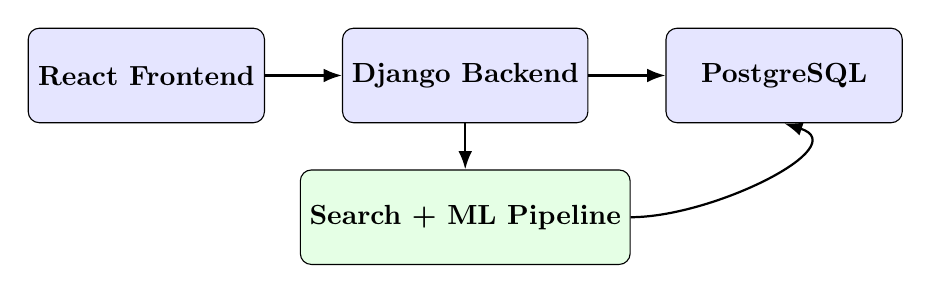
\begin{tikzpicture}[scale=0.9]
  \node[draw,rounded corners,fill=blue!10,minimum width=3cm,minimum height=1.2cm] (fe)
    at (0,0) {\bfseries React Frontend};
  \node[draw,rounded corners,fill=blue!10,minimum width=3cm,minimum height=1.2cm] (be)
    at (4.5,0) {\bfseries Django Backend};
  \node[draw,rounded corners,fill=blue!10,minimum width=3cm,minimum height=1.2cm] (db)
    at (9,0) {\bfseries PostgreSQL};
  \node[draw,rounded corners,fill=green!10,minimum width=3cm,minimum height=1.2cm] (ml)
    at (4.5,-2) {\bfseries Search + ML Pipeline};
  \draw[-Latex,thick] (fe) -- (be);
  \draw[-Latex,thick] (be) -- (db);
  \draw[-Latex,thick] (be) -- (ml);
  \draw[-Latex,thick] (ml.east) .. controls (8,-2) and (10,-1) .. (db.south);
\end{tikzpicture}

\vfill

{\large\itshape Covers: Django 4.2, DRF, PostgreSQL, React 18, Tailwind CSS,\\
LightGBM LambdaRank, SetFit intent classifier, semantic embeddings,\\
Node2Vec graphs, Docker, ngrok, end-to-end SaaS subscriptions.}

\vspace{1.5cm}

{\large Compiled for the Zarailink team --- May 2026}\\[6pt]
{\small Build target: \fileref{zarailink_guide.pdf}}
\end{titlepage}

% ----- Front matter -------------------------------------------------
\frontmatter
% ===== inlined from chapters/00_preface.tex =====
\chapter*{Preface}
\addcontentsline{toc}{chapter}{Preface}
\markboth{Preface}{Preface}

\section*{Who is this guide for?}

This document was written with one specific reader in mind: \textbf{a complete
beginner who has just been handed the Zarailink codebase} and asked to make
sense of it. Maybe you are a new team member joining the project. Maybe you
are evaluating it as a final-year-project (FYP) supervisor. Maybe you are a
student studying full-stack data products and want a worked example. In all
of these cases, you should be able to read this guide top-to-bottom, with no
prior knowledge of Django, React, machine learning, or the Pakistani
agricultural trade domain, and emerge with a complete operational
understanding of every moving part.

\section*{What "complete" means here}

Most software guides paraphrase the code. This one does not. Wherever
practical, we quote the \emph{actual} source --- with the file path and the
exact line numbers --- so you can open the file in your editor and follow
along. Wherever a function uses a non-obvious algorithm (e.g. the LambdaRank
loss in the Learning-to-Rank model), we explain the algorithm before we
explain the code. Wherever a configuration value matters (e.g. the
\inlinecode{SESSION\_COOKIE\_AGE} setting), we tell you not just what value it
holds but \emph{why that value was chosen} and what would break if it
changed.

\begin{noviceBox}
You do not need to read this guide in order. Skim Chapter~1
(\textbf{Introduction}) and Chapter~3 (\textbf{Architecture}) first to get
the lay of the land. Then jump to whichever chapter matches the work you are
about to do.
\end{noviceBox}

\section*{How to use this guide}

\textbf{Code blocks} look like this:

\begin{lstlisting}[language=Python,caption={A code block}]
def hello(name: str) -> str:
    return f"Hello, {name}!"
\end{lstlisting}

\textbf{File references} look like this: \fileref{backend/zarailink/settings.py}.
When we cite a particular line, we write \fileref{backend/zarailink/settings.py:209}
which means \emph{settings.py, line 209}. You can almost always
\inlinecode{Ctrl-G} (Go to Line) in your editor to jump straight there.

\textbf{Coloured boxes} flag content that needs special attention:

\begin{noviceBox}
\textbf{Beginner Note} --- background you might be missing if you have never
worked in this kind of codebase before.
\end{noviceBox}

\begin{warnBox}
\textbf{Warning} --- a footgun. Things that have broken before, or that will
break if you change them carelessly.
\end{warnBox}

\begin{tipBox}
\textbf{Tip} --- a shortcut, an idiom, or a way to save yourself an hour.
\end{tipBox}

\begin{exampleBox}
\textbf{Worked Example} --- a concrete walkthrough of a real query, request,
or workflow with sample data.
\end{exampleBox}

\begin{whyBox}
\textbf{Why This Matters} --- design rationale. Why the team chose option A
over option B, and what tradeoff they accepted.
\end{whyBox}

\section*{Conventions}

\begin{itemize}
  \item \textbf{Paths} are written relative to the repository root, which we
        write as \fileref{Zarailink-Code/}.
  \item \textbf{Shell commands} prefixed with \inlinecode{\$} are user-level;
        commands prefixed with \inlinecode{\#} require root.
  \item Where the project ships its own scripts, we prefer them
        (e.g.~\inlinecode{./setup\_linux.sh}) over manual commands so that
        you stay aligned with the team.
  \item URLs are clickable in the PDF. Any link to localhost (e.g.
        \inlinecode{http://localhost:8000}) assumes you have followed the
        setup chapter.
\end{itemize}

\section*{Source-of-truth disclaimer}

Software changes. The exact line numbers in this guide were captured against
the commit on branch \inlinecode{umar\_branch2} (HEAD as of compilation). If a
line number is off by a few when you read it, the surrounding context will
still help you find the right code. The \emph{behaviour} described, however,
matches the source files committed to that branch and the corresponding ML
artefacts in \fileref{backend/models/} and \fileref{backend/search/models/}.

If you spot an inaccuracy --- a feature documented here that no longer
exists, an endpoint that has been renamed --- treat the source code as the
authoritative answer and update this guide.
% ===== end chapters/00_preface.tex =====

\tableofcontents
\listoffigures
\listoftables

% ----- Main matter --------------------------------------------------
\mainmatter

% ===== inlined from chapters/01_introduction.tex =====
\chapter{Introduction}
\label{ch:intro}

\section{What is Zarailink?}

\textbf{Zarailink} is a Software-as-a-Service (SaaS) platform that turns
millions of raw \emph{customs trade records} from Pakistan into something a
human can act on: lists of suppliers and buyers, charts of price trends,
contact unlocks, and a search experience that understands natural-language
queries like \emph{``cheap rice exporters to UAE under \$0.40/kg.''}

The product targets three user personas:

\begin{itemize}
  \item \textbf{Importers} (foreign buyers) who want to discover Pakistani
        suppliers of a specific commodity at a target price point.
  \item \textbf{Exporters} (Pakistani sellers) who want to discover overseas
        buyers, evaluate competitive landscapes, and price their goods.
  \item \textbf{Analysts and trade officers} who use the platform's
        analytics, network graphs, and watchlists for market intelligence.
\end{itemize}

\begin{noviceBox}
A \textbf{customs trade record} is the line-item that a customs authority
files for every shipment crossing a border. It typically includes the
shipper, the consignee, the country, the HS code (a worldwide product
taxonomy), the volume, and the declared price. Pakistan's official customs
data is a goldmine of business intelligence; Zarailink makes that goldmine
queryable.
\end{noviceBox}

\section{The "elevator pitch" architecture}

At the highest level, Zarailink is a typical \emph{three-tier web
application}, but with a powerful machine-learning search engine bolted
between the database and the API layer:

\begin{enumerate}
  \item A \textbf{React} single-page application (SPA) in the browser, built
        with Tailwind CSS for styling and Recharts/Framer Motion for
        visualisations and animations.
  \item A \textbf{Django + Django REST Framework (DRF)} backend that exposes
        REST endpoints, manages authentication, subscriptions, and the
        token-balance economy for unlocking key contacts.
  \item A \textbf{PostgreSQL} database holding the structured trade
        ledger, company directory, user accounts, and subscription plans.
  \item A \textbf{search-and-ranking subsystem} that sits inside the Django
        backend and runs a four-stage ML pipeline (NLU $\rightarrow$
        retrieval $\rightarrow$ aggregation $\rightarrow$ ranking) every
        time the user submits a query.
\end{enumerate}

\begin{figure}[h]
\centering
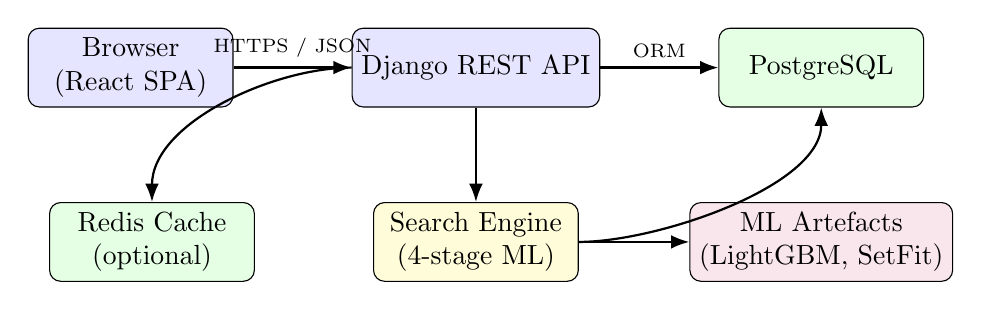
\begin{tikzpicture}[node distance=1.2cm and 1.5cm,
    box/.style={draw,rounded corners,minimum width=2.6cm,minimum height=1cm,align=center},
    blueb/.style={fill=blue!10},
    greenb/.style={fill=green!10},
    yellowb/.style={fill=yellow!15},
    purpleb/.style={fill=purple!10},
    arrow/.style={-Latex,thick}]
  \node[box,blueb] (browser) {Browser\\ (React SPA)};
  \node[box,blueb,right=of browser] (api) {Django REST API};
  \node[box,greenb,right=of api] (db) {PostgreSQL};
  \node[box,yellowb,below=of api] (search) {Search Engine\\ (4-stage ML)};
  \node[box,purpleb,below=of db] (artifacts) {ML Artefacts\\ (LightGBM, SetFit)};
  \node[box,greenb,left=of search] (cache) {Redis Cache\\ (optional)};

  \draw[arrow] (browser) -- node[above,font=\scriptsize]{HTTPS / JSON} (api);
  \draw[arrow] (api) -- node[above,font=\scriptsize]{ORM} (db);
  \draw[arrow] (api) -- (search);
  \draw[arrow] (search) -- (artifacts);
  \draw[arrow] (search.east) .. controls +(1,0) and +(0,-1) .. (db.south);
  \draw[arrow] (api.west) .. controls +(-1,0) and +(0,1) .. (cache.north);
\end{tikzpicture}
\caption{Bird's-eye view of the Zarailink runtime topology.}
\label{fig:bird-eye}
\end{figure}

\begin{whyBox}
The team chose to embed the search ML \emph{inside} the Django process
rather than running it as a separate microservice. The trade-off: simpler
deployment and zero network hop, at the cost of a heavier worker process
(LightGBM, SentenceTransformer, and SetFit are all loaded in memory). For a
final-year project where ops simplicity matters more than horizontal
scalability, this was the right call.
\end{whyBox}

\section{The four-stage search pipeline}
\label{sec:intro-pipeline}

Search is the core differentiator of Zarailink, so let us preview the
pipeline now (we devote all of Chapter~\ref{ch:search-engine} to it).

\begin{description}
  \item[Stage 1 --- QueryInterpreter (NLU).] Takes the raw query string
        (e.g.~\emph{``looking for cheap basmati rice from Punjab to Dubai''})
        and returns a \emph{structured intent}: an action (\inlinecode{BUY}
        / \inlinecode{SELL}), a product list, country filters, price
        operators, and so on. Implemented in
        \fileref{backend/search/services/nlu_engine.py} (1{,}305 lines).
  \item[Stage 2 --- QueryMatcher.] Converts the structured intent into a
        list of \inlinecode{ProductSubCategory} IDs by combining
        \emph{keyword matches} (BM25), \emph{semantic matches} (sentence
        embeddings) and \emph{fuzzy matches} (RapidFuzz). Implemented in
        \fileref{backend/search/services/candidate_retrieval.py}.
  \item[Stage 3 --- SupplierAggregator.] Runs a heavy-duty Django ORM
        aggregation over the \inlinecode{Transaction} table to roll up
        per-supplier metrics: weighted average price, total volume,
        shipment frequency, repeat-customer ratio. Implemented in
        \fileref{backend/search/services/aggregation.py} (1{,}462 lines).
  \item[Stage 4 --- RankingEnsemble.] Ranks the suppliers via a 70/30
        blend: 70\% \emph{heuristic} score (volume, recency, price-fit) and
        30\% \emph{LightGBM LambdaRank} model trained on pseudo-labels.
        Implemented in \fileref{backend/search/services/ranking.py} and
        \fileref{backend/search/services/ranking_ltr.py}.
\end{description}

The trained LTR model lives at \fileref{backend/search/models/lgbm_ltr.txt}
and the SetFit intent classifier at \fileref{backend/models/zarai_intent_model/}.

\section{Tech stack at a glance}

\begin{table}[h]
\centering
\small
\begin{tabular}{p{3.2cm} p{4.5cm} p{6.0cm}}
\toprule
\textbf{Layer} & \textbf{Technology} & \textbf{Where to find it} \\
\midrule
Frontend framework  & React 18 (CRA) & \fileref{frontend/src/} \\
Frontend styling    & Tailwind CSS, custom CSS modules & \fileref{frontend/tailwind.config.js} \\
Charts \& animations & Recharts, Framer Motion & \fileref{frontend/src/components/} \\
HTTP client         & Axios & \fileref{frontend/src/services/api.js} \\
Backend framework   & Django 4.2 + DRF 3.14 & \fileref{backend/zarailink/} \\
Auth                & Session-based (\inlinecode{accounts.User}) & \fileref{backend/accounts/} \\
Subscriptions       & Custom token-balance economy & \fileref{backend/subscriptions/} \\
Database            & PostgreSQL 14+ & local server, see Setup \\
Caching             & Redis (optional) or LocMem fallback & \fileref{backend/zarailink/settings.py:115} \\
NLU intent          & SetFit (BAAI/bge-small-en-v1.5) & \fileref{backend/models/zarai_intent_model/} \\
NER                 & GLiNER (zero-shot) & loaded in \fileref{nlu_engine.py} \\
Embeddings          & SentenceTransformer (384-d) & loaded in \fileref{vector_store.py} \\
LTR ranking         & LightGBM LambdaRank & \fileref{backend/search/models/lgbm_ltr.txt} \\
Graph features      & networkx + Node2Vec & \fileref{backend/*.graphml} \\
Optional LLM        & OpenRouter / OpenAI & \fileref{backend/utils/ai_service.py} \\
Container           & Docker + docker-compose & \fileref{docker-compose.yml} \\
Tunnelling          & ngrok (dev demo) & \fileref{backend/ngrok.exe} \\
\bottomrule
\end{tabular}
\caption{Zarailink technology stack.}
\label{tab:stack}
\end{table}

\begin{noviceBox}
\textbf{What is "session-based" auth?} When you log in, Django stores a
small server-side record (a "session") and sends your browser a cookie
containing the session ID. On every subsequent request, the browser sends
the cookie back; Django looks up the session, and knows who you are. This is
the simplest auth model and what Zarailink uses despite the
\inlinecode{djangorestframework-simplejwt} package being listed in
\fileref{requirements.txt} --- the JWT plumbing is installed but not wired up.
\end{noviceBox}

\section{The Django apps you will encounter}

A Django project is divided into \emph{apps}, each owning a set of models,
views and URL routes. Zarailink has these:

\begin{table}[h]
\centering
\small
\begin{tabular}{p{3.0cm} p{11cm}}
\toprule
\textbf{App} & \textbf{Responsibility} \\
\midrule
\inlinecode{accounts}        & Custom \inlinecode{User} model, signup, email verification, login, password reset, profile, audit log. \\
\inlinecode{subscriptions}   & Subscription plans, redeem codes, key-contact unlocks (token economy). \\
\inlinecode{companies}       & The company directory, sectors, key contacts, watchlist. \\
\inlinecode{trade_data}     & The \inlinecode{Transaction} ledger and trade aggregates. \\
\inlinecode{search}          & API surface for the search engine; orchestrates the four-stage pipeline. \\
\inlinecode{home}            & Empty placeholder app. \\
\inlinecode{trade_directory} & Empty placeholder app. \\
\inlinecode{trade_lens}     & Trade-graph / network analysis (loaded but no Django app, mostly utility code). \\
\inlinecode{trade_ledger}   & Same: utility code, not a Django app. \\
\inlinecode{market_intel}   & Market-intelligence helpers; mostly empty. \\
\bottomrule
\end{tabular}
\caption{Django apps and their roles.}
\label{tab:apps}
\end{table}

The \emph{empty} apps (\inlinecode{home}, \inlinecode{trade_directory})
exist as placeholders for future expansion --- the team scaffolded them
early but the corresponding features moved into the existing apps. This is
worth noting because at first glance the app list suggests more
functionality than the code actually contains; do not be misled.

\section{What you can do with Zarailink (user-facing tour)}

The frontend exposes the following pages (all routed through
\fileref{frontend/src/App.js}):

\begin{itemize}
  \item \textbf{Landing page} (\inlinecode{/}) --- marketing copy.
  \item \textbf{Signup / Login / Forgot Password} (\inlinecode{/signup},
        \inlinecode{/login}, \inlinecode{/forgot}, \inlinecode{/reset/<token>}).
  \item \textbf{Dashboard} (\inlinecode{/dashboard}) --- charts of top
        commodities, top trade partners, monthly trends.
  \item \textbf{Search} (\inlinecode{/search}) --- natural-language search
        with results, side filters, sort, pagination.
  \item \textbf{Deal Detail} (\inlinecode{/search/deal/:id}) --- the
        massive 1{,}688-line component that shows everything about a single
        supplier-product pair: price history, partners, key contacts,
        verification status, watchlist toggle.
  \item \textbf{Compare} (\inlinecode{/search/compare}) --- side-by-side
        comparison of multiple suppliers.
  \item \textbf{Data Dashboard} (\inlinecode{/search/data}) --- a heavier
        analytical view with charts.
  \item \textbf{Trade Directory} (\inlinecode{/find-buyers},
        \inlinecode{/find-suppliers}, \inlinecode{/company/:id}) --- the
        searchable directory of companies, with a deep profile per company.
  \item \textbf{Trade Intelligence} (\inlinecode{/intelligence/...}) ---
        company overview, partners, products, link prediction (graph ML).
  \item \textbf{Watchlist} (\inlinecode{/watchlist}) --- the user's saved
        companies/products.
  \item \textbf{Subscriptions} (\inlinecode{/subscription}) --- plan
        selection, redeem code entry.
  \item \textbf{User Profile} (\inlinecode{/profile}) --- account settings,
        token balance, audit log.
\end{itemize}

\section{Roadmap of this guide}

\begin{description}
  \item[Chapter \ref{ch:intro}.] You are here.
  \item[Chapter \ref{ch:setup}.] Setting up the project on your laptop, end
        to end. Choose Linux, macOS, or Windows; we walk through every
        prerequisite, every command, every common error.
  \item[Chapter \ref{ch:arch}.] The full architecture: a traced
        request-response, the database schema, and the pipeline contracts
        between modules.
  \item[Chapter \ref{ch:backend}.] The Django backend: every app, every
        model, every endpoint.
  \item[Chapter \ref{ch:search-engine}.] The search engine and the entire
        ML pipeline. NLU, retrieval, aggregation, ranking, training.
  \item[Chapter \ref{ch:frontend}.] The React frontend: every component,
        every hook, every API call.
  \item[Chapter \ref{ch:data}.] The data layer: Excel files, JSON
        fixtures, GraphML files, ingestion scripts, ML model artefacts.
  \item[Chapter \ref{ch:deploy}.] Deployment and operations: Docker,
        ngrok, setup scripts, environment variables.
  \item[Chapter \ref{ch:testing}.] How the project is tested, plus how to
        add your own tests.
  \item[Chapter \ref{ch:trouble}.] Troubleshooting common errors.
  \item[Appendices.] Glossary, API endpoint reference, model field
        reference, the quality checklist used to verify this guide, and
        external resources.
\end{description}

\begin{tipBox}
A useful first action: open \fileref{COMPLETE_SYSTEM_GUIDE.md} (in the
project root) in parallel with this PDF. That markdown file is the team's
internal Wiki; this PDF is the structured deep-dive that complements it.
\end{tipBox}
% ===== end chapters/01_introduction.tex =====

% ===== inlined from chapters/02_setup.tex =====
\chapter{Setup --- From Zero to Running}
\label{ch:setup}

This chapter walks you all the way from a fresh laptop to a running
Zarailink instance with the React UI live in your browser. We assume
\emph{nothing}: every command, every prerequisite, every gotcha is
covered. If you have already done parts of this, skim --- the section
headings make it easy to skip.

\section{Hardware and OS}

Zarailink will run on any modern 64-bit machine. For comfort:

\begin{itemize}
  \item \textbf{RAM:} 8\,GB is the floor; 16\,GB is the recommended
        minimum. The ML pipeline (LightGBM + SetFit + SentenceTransformer)
        loads several hundred MB into the Django process.
  \item \textbf{Disk:} reserve $\sim$8\,GB. The \fileref{backend/.venv/}
        directory alone is roughly 4\,GB after \inlinecode{pip install -r requirements.txt}
        (PyTorch, Transformers and friends are large).
  \item \textbf{CPU:} any 4-core x86\_64 or Apple Silicon CPU. No GPU is
        required for the search inference path; if you happen to have a
        CUDA-capable GPU, PyTorch will use it for embeddings, but the
        project ships fine on CPU.
  \item \textbf{OS:} Ubuntu 22.04+ / Debian 12+ / Fedora 39+ on Linux;
        macOS Sonoma or later (Intel or Apple Silicon); Windows 10/11 with
        WSL2 strongly recommended.
\end{itemize}

\section{Prerequisites}

You must install five pieces of system software before you touch the repo.
The official requirements (mirrored from \fileref{SETUP.md}) are:

\begin{table}[h]
\centering
\small
\begin{tabular}{p{3cm} p{2.5cm} p{8cm}}
\toprule
\textbf{Tool} & \textbf{Min version} & \textbf{Why we need it} \\
\midrule
Python      & 3.12+      & Backend runtime; \fileref{requirements.txt} pins newer-style typing. \\
Node.js     & 18 (LTS)+  & Builds and serves the React frontend; the project also uses \emph{Puppeteer} (which needs Node) for PDF export. \\
npm         & 9+         & Comes with Node.js; installs frontend deps. \\
Docker      & latest     & Runs Redis Stack as a container (see \fileref{backend/docker-compose.yml}). \\
PostgreSQL  & 15+        & Primary database; required even for local dev. \\
\bottomrule
\end{tabular}
\caption{Prerequisite software versions.}
\label{tab:prereqs}
\end{table}

\subsection{Linux (Ubuntu 22/24): one-shot install}

\begin{lstlisting}[language=Bash,caption={Installing all prereqs on Ubuntu}]
# 1. System tools
sudo apt update
sudo apt install -y build-essential git curl

# 2. Python 3.12 (Ubuntu 24.04 ships with 3.12 by default)
sudo apt install -y python3 python3-venv python3-pip

# 3. Node.js 18 LTS via NodeSource
curl -fsSL https://deb.nodesource.com/setup_18.x | sudo -E bash -
sudo apt install -y nodejs

# 4. PostgreSQL 15+
sudo apt install -y postgresql postgresql-contrib
sudo systemctl enable --now postgresql

# 5. Docker
sudo apt install -y docker.io docker-compose-plugin
sudo systemctl enable --now docker
sudo usermod -aG docker "$USER"   # log out and back in to pick this up
\end{lstlisting}

\begin{warnBox}
The \inlinecode{usermod -aG docker} change does not take effect until you
\textbf{log out and back in} (or reboot). If \inlinecode{docker info}
returns a permission error, that is why.
\end{warnBox}

\subsection{macOS (Apple Silicon or Intel)}

\begin{lstlisting}[language=Bash,caption={Installing prereqs via Homebrew}]
# Homebrew itself
/bin/bash -c "$(curl -fsSL https://raw.githubusercontent.com/Homebrew/install/HEAD/install.sh)"

# The five tools
brew install python@3.12 node@18 postgresql@15
brew services start postgresql@15
# Docker Desktop comes from a .dmg installer, not brew
# https://www.docker.com/products/docker-desktop/
\end{lstlisting}

\subsection{Windows 10/11}

You have two equally valid paths:

\begin{enumerate}
  \item \textbf{Native Windows:} install Python from
        \inlinecode{python.org}, Node.js from \inlinecode{nodejs.org}, the
        PostgreSQL EDB installer, and Docker Desktop. Use the
        \fileref{setup_windows.ps1} script as your single source of truth.
  \item \textbf{WSL2 + Ubuntu:} run the entire stack inside WSL2 and
        treat your machine as Linux. This is the team's recommendation
        because the \fileref{setup_linux.sh} script just works.
\end{enumerate}

\section{Cloning the repo}

\begin{lstlisting}[language=Bash,caption={Cloning Zarailink}]
git clone <your-fork-url> Zarailink-Code
cd Zarailink-Code
\end{lstlisting}

The repository root contains \fileref{backend/}, \fileref{frontend/}, the
three setup scripts, and a wealth of documentation \fileref{*.md} files.

\section{The fast path: automated setup scripts}

The Zarailink team ships three idempotent setup scripts. Idempotent means
\emph{you can run them again and again} --- they skip steps that are already
done. Pick the one for your OS:

\begin{table}[h]
\centering
\small
\begin{tabular}{p{2.5cm} p{5.5cm} p{5.5cm}}
\toprule
\textbf{OS} & \textbf{Command} & \textbf{Script} \\
\midrule
Linux         & \fileref{./setup_linux.sh}      & \fileref{setup_linux.sh} (395 lines) \\
macOS         & \fileref{./setup_mac.sh}        & \fileref{setup_mac.sh} \\
Windows       & \fileref{.\setup_windows.ps1} (PowerShell)  & \fileref{setup_windows.ps1} \\
\bottomrule
\end{tabular}
\end{table}

On Linux/macOS make the script executable first:

\begin{lstlisting}[language=Bash,caption={Marking the script executable}]
chmod +x setup_linux.sh   # or setup_mac.sh
./setup_linux.sh
\end{lstlisting}

\subsection{What the Linux script actually does}

If you want to know what is happening under the hood (and you should ---
this is your codebase now), here is the play-by-play of
\fileref{setup_linux.sh}, broken down section by section:

\begin{description}
  \item[Lines 66--128 --- pre-flight checks.] Verifies that
        \inlinecode{python3}, \inlinecode{python3-venv}, \inlinecode{node},
        \inlinecode{npm}, \inlinecode{docker}, and \inlinecode{psql} all
        exist. Bails out with a friendly install hint if any are missing.
  \item[Lines 138--157 --- virtualenv.] Creates
        \fileref{backend/.venv/} via \inlinecode{python3 -m venv .venv}.
        If a venv exists but is broken (missing \inlinecode{bin/activate}),
        it deletes and recreates.
  \item[Lines 161--191 --- pip install.] Activates the venv and runs
        \inlinecode{pip install -r requirements.txt}. This installs $\sim$120
        packages including Django, DRF, LightGBM, SentenceTransformers,
        SetFit, GLiNER, KeyBERT, OpenSearch, and more. \emph{Allow up to 5
        minutes here.}
  \item[Lines 194--207 --- .env file.] Copies \fileref{backend/.env.example}
        to \fileref{backend/.env} and generates a fresh
        \inlinecode{SECRET_KEY} via Django's helper.
  \item[Lines 215--228 --- PostgreSQL database.] Calls
        \inlinecode{sudo -u postgres createdb zarailink} and sets the
        \inlinecode{postgres} user's password to \inlinecode{postgres} (yes,
        really --- it is hardcoded in \fileref{settings.py:105}).
  \item[Lines 231--237 --- migrations and roles.] Runs
        \inlinecode{python manage.py migrate} to create all tables, then
        \inlinecode{python manage.py setup_company_roles} to seed the
        company-role lookup data.
  \item[Lines 244--251 --- sample company data.] If
        \fileref{backend/load_data.py} exists and the
        \inlinecode{Company} table is empty, loads sample data.
  \item[Lines 257--266 --- trade transactions.] If
        \fileref{import_data_1year.xlsx} exists at the repo root, ingests
        it via \inlinecode{python manage.py ingest_trade --file ...}. This
        populates the \inlinecode{Transaction} table that the search engine
        and dashboards depend on.
  \item[Lines 269--297 --- GNN graphs and embeddings.] If transactions
        exist, builds the \fileref{*.graphml} files via
        \inlinecode{build_gnn_graphs} and the
        \inlinecode{CompanyEmbedding} rows via
        \inlinecode{generate_gnn_embeddings --fast}. These power the
        ``Similar Companies'' feature.
  \item[Lines 305--320 --- Redis container.] Starts
        \fileref{backend/docker-compose.yml} which launches a
        \inlinecode{redis/redis-stack:latest} container named
        \inlinecode{zarailink-redis} on port \inlinecode{6379} (data) and
        \inlinecode{8001} (Redis Insight UI).
  \item[Lines 327--336 --- frontend npm install.] \inlinecode{cd ../frontend && npm install --legacy-peer-deps}
        installs React, Tailwind, Recharts, etc.
  \item[Lines 343--351 --- Puppeteer.] In \fileref{backend/}, a tiny
        \fileref{package.json} pulls in Puppeteer for server-side PDF
        generation (used by the report-export endpoints).
  \item[Lines 358--393 --- summary banner.] Prints the next-step commands
        and access URLs.
\end{description}

\begin{tipBox}
If the script bails out part-way through, you can rerun it. It will pick
up where it left off thanks to the idempotency checks. The most common
failure is the \inlinecode{pip install} step running out of memory on small
VMs --- swap or upgrade to 8\,GB+ RAM.
\end{tipBox}

\section{The slow path: manual setup}

If the automated script does not work for you (corporate firewall,
custom OS, etc.), here is the equivalent step-by-step you can run by
hand.

\subsection{Backend}

\begin{lstlisting}[language=Bash,caption={Manual backend setup}]
cd backend

# 1. Virtual environment
python3 -m venv .venv
source .venv/bin/activate     # on Windows: .\.venv\Scripts\Activate.ps1

# 2. Dependencies
pip install --upgrade pip
pip install -r requirements.txt

# 3. Environment file
cp .env.example .env

# 4. Generate a SECRET_KEY and paste it into .env
python -c "from django.core.management.utils import get_random_secret_key; print(get_random_secret_key())"

# 5. Database
sudo -u postgres createdb zarailink   # Linux
# brew: createdb zarailink             # macOS
# Windows: createdb -U postgres zarailink

# 6. Apply migrations
python manage.py migrate

# 7. Optional: superuser for /admin
python manage.py createsuperuser

# 8. Seed lookup tables
python manage.py setup_company_roles

# 9. Optional: load sample companies
python load_data.py

# 10. Run the dev server
python manage.py runserver 0.0.0.0:8000
\end{lstlisting}

\subsection{Frontend}

\begin{lstlisting}[language=Bash,caption={Manual frontend setup}]
cd frontend
npm install --legacy-peer-deps
npm start
\end{lstlisting}

\subsection{Redis (optional but recommended)}

\begin{lstlisting}[language=Bash,caption={Starting Redis via Docker}]
cd backend
docker compose up -d         # newer Docker
# or
docker-compose up -d         # older Docker
\end{lstlisting}

\begin{noviceBox}
Redis is \textbf{optional}. \fileref{backend/zarailink/settings.py:115-143}
contains an \inlinecode{is_redis_available()} check that opens a TCP socket
to \inlinecode{127.0.0.1:6379}. If Redis is up, Django uses
\inlinecode{django_redis.cache.RedisCache}. If it is down, Django silently
falls back to in-process \inlinecode{LocMemCache}. So you can develop
without Docker; you just lose cross-process cache sharing and the NLU cache
benefit.
\end{noviceBox}

\section{The .env file (the most-edited file in your life)}

The setup script copies \fileref{backend/.env.example} to
\fileref{backend/.env}. Here is the full list of variables and what they
do, cross-checked against \fileref{backend/zarailink/settings.py}:

\begin{table}[h]
\centering
\small
\begin{tabular}{p{4cm} p{1.4cm} p{8cm}}
\toprule
\textbf{Variable} & \textbf{Required?} & \textbf{Effect} \\
\midrule
\inlinecode{SECRET_KEY}        & \textbf{Yes} & Django cryptographic signing key. Read at \fileref{settings.py:28}. \\
\inlinecode{OPENROUTER_API_KEY} & No          & Used by \fileref{utils/ai_service.py} for the LLM-backed price extraction fallback. \fileref{settings.py:30}. \\
\inlinecode{OPENAI_KEY}        & No          & Used for ``AI Smart Search'' and the OpenAI embedding fallback. \fileref{settings.py:146}. \\
\inlinecode{EMAIL_HOST_USER}   & No          & Gmail address for outbound email (verification, password reset). \fileref{settings.py:327}. \\
\inlinecode{EMAIL_HOST_PASSWORD} & No        & Gmail \textbf{App Password}, not your regular password. \\
\inlinecode{FRONTEND_URL}      & No          & Used inside email templates so that ``Verify your account'' links point to the correct host. Defaults to \inlinecode{http://localhost:3000}. \fileref{settings.py:332}. \\
\bottomrule
\end{tabular}
\end{table}

\subsection{Generating a SECRET\_KEY}

\begin{lstlisting}[language=Bash,caption={One-liner for SECRET\_KEY}]
cd backend && source .venv/bin/activate
python -c "from django.core.management.utils import get_random_secret_key; print(get_random_secret_key())"
\end{lstlisting}

Copy the output into \fileref{backend/.env} as
\inlinecode{SECRET_KEY=django-insecure-xxxxxxxxxxxxxxxxxxxxxx}.

\subsection{Setting up Gmail App Passwords}

If you want email verification to work end-to-end, you need a Gmail
App Password (the kind that is immune to 2FA prompts):

\begin{enumerate}
  \item Visit \url{https://myaccount.google.com/security} and turn on
        \emph{2-Step Verification} (cannot generate App Passwords without it).
  \item Visit \url{https://myaccount.google.com/apppasswords}.
  \item Create a new App Password called ``Zarailink''. Copy the 16
        characters Google gives you.
  \item Paste it into \fileref{.env} as \inlinecode{EMAIL_HOST_PASSWORD},
        with no spaces.
\end{enumerate}

\begin{warnBox}
Do \textbf{not} commit your \fileref{.env} file. It is already listed in
\fileref{.gitignore}. If you accidentally commit it, rotate every secret
inside.
\end{warnBox}

\section{Running the application}

Three terminals, three commands:

\begin{lstlisting}[language=Bash,caption={Terminal 1: Redis (optional)}]
cd backend
docker compose up -d
\end{lstlisting}

\begin{lstlisting}[language=Bash,caption={Terminal 2: Django backend}]
cd backend
source .venv/bin/activate
python manage.py runserver 0.0.0.0:8000
\end{lstlisting}

\begin{lstlisting}[language=Bash,caption={Terminal 3: React frontend}]
cd frontend
npm start
\end{lstlisting}

After a few seconds you can open the URLs in
Table~\ref{tab:urls}.

\begin{table}[h]
\centering
\small
\begin{tabular}{p{4cm} p{8cm}}
\toprule
\textbf{Service} & \textbf{URL} \\
\midrule
Frontend (React)        & \url{http://localhost:3000} \\
Backend API (DRF)       & \url{http://localhost:8000/api/} \\
Django admin            & \url{http://localhost:8000/admin/} \\
Redis Insight UI        & \url{http://localhost:8001} \\
DRF browsable login     & \url{http://localhost:8000/api-auth/login/} \\
CKEditor 5 endpoint     & \url{http://localhost:8000/ckeditor5/} \\
\bottomrule
\end{tabular}
\caption{Local URLs after a successful setup.}
\label{tab:urls}
\end{table}

\section{Smoke test: am I really running?}

Six checks --- if all six pass, you have a working install.

\begin{enumerate}
  \item \inlinecode{curl http://localhost:8000/admin/} returns HTML
        containing the Django log-in page.
  \item \inlinecode{curl http://localhost:8000/api/} returns a JSON 401
        (auth required) or 200 with route hints --- both are fine.
  \item Open \url{http://localhost:3000} --- you see the Zarailink landing
        page styled with Tailwind.
  \item Sign up at \url{http://localhost:3000/signup}; you receive a verify
        email if SMTP is configured (or you skip verification by setting
        \inlinecode{is_verified=True} in the admin).
  \item Visit \url{http://localhost:3000/dashboard} after login: you see
        charts (they may be empty if you skipped data ingestion).
  \item Type a query in the search box at \url{http://localhost:3000/search}
        --- you receive results within $\sim$2\,seconds.
\end{enumerate}

\section{Loading the data}
\label{sec:setup-data}

A search engine without data is just a spinning wheel. The repo ships
sample fixtures and Excel files which you can ingest:

\begin{lstlisting}[language=Bash,caption={Loading sample data}]
cd backend && source .venv/bin/activate

# Companies + sectors + roles
python manage.py setup_company_roles
python load_data.py

# Trade transactions (import side)
python manage.py ingest_trade --file ../import_data_1year.xlsx

# Trade transactions (export side)
python manage.py ingest_trade_export --file ../export_data.xlsx

# Build the search index pickle
python manage.py build_search_index

# Optional: GNN graphs and embeddings (enables Similar Companies)
python manage.py build_gnn_graphs
python manage.py generate_gnn_embeddings --fast
\end{lstlisting}

We dedicate Chapter~\ref{ch:data} to a deep dive on these data files,
their schemas, and the ingestion pipeline.

\section{Common setup failures}

We collect the recurring failure modes here so you can find them by
\inlinecode{Ctrl-F} and move on.

\begin{description}
  \item[\inlinecode{ModuleNotFoundError: No module named 'django'}.] You
        forgot \inlinecode{source .venv/bin/activate}.
  \item[\inlinecode{FATAL: database "zarailink" does not exist}.] Run
        \inlinecode{sudo -u postgres createdb zarailink} (Linux) or
        \inlinecode{createdb zarailink} (macOS).
  \item[\inlinecode{FATAL: password authentication failed for user "postgres"}.]
        Run \inlinecode{sudo -u postgres psql -c "ALTER USER postgres PASSWORD 'postgres';"}.
        Yes, the password is hardcoded.
  \item[Redis connection refused.] Either start the container
        (\inlinecode{docker compose up -d} from \fileref{backend/}) or
        ignore --- Django will fall back to LocMemCache.
  \item[\inlinecode{npm ERR! ERESOLVE unable to resolve dependency tree}.]
        Re-run with \inlinecode{npm install --legacy-peer-deps}.
  \item[\inlinecode{pip install} stalls on \inlinecode{torch}.] Torch
        wheels are large ($\sim$700\,MB). Be patient, or pre-install
        \inlinecode{torch==2.1.0} from the PyTorch index.
  \item[\inlinecode{psql: command not found}.] Add the PostgreSQL
        \inlinecode{bin} folder to your \inlinecode{PATH}.
  \item[Browser shows \inlinecode{CSRF verification failed}.] Make sure
        \inlinecode{CORS_ALLOW_CREDENTIALS=True} (it is, in
        \fileref{settings.py:349}) and that the frontend dev server is on
        \inlinecode{localhost:3000}, not \inlinecode{127.0.0.1:3000}.
\end{description}

\section{Demoing on a public URL with ngrok}

The repo ships \fileref{backend/ngrok.exe} (Windows) so the team can
quickly expose \inlinecode{localhost:8000} during demos. The settings
file already whitelists ngrok hosts at \fileref{settings.py:36}:

\begin{lstlisting}[language=Python,caption={ngrok-friendly ALLOWED\_HOSTS},firstnumber=36]
ALLOWED_HOSTS = ['localhost', '127.0.0.1', '.ngrok-free.dev', '.ngrok-free.app']
\end{lstlisting}

To run a demo tunnel:

\begin{lstlisting}[language=Bash,caption={Public ngrok tunnel}]
ngrok http 8000   # gives you a https://xxxx.ngrok-free.app URL
\end{lstlisting}

You should now have a fully running Zarailink stack on your machine.
The next chapter zooms out and explains \emph{how} all the pieces talk
to each other.
% ===== end chapters/02_setup.tex =====

% ===== inlined from chapters/03_architecture.tex =====
\chapter{Architecture --- The Big Picture}
\label{ch:arch}

Now that you can run Zarailink, this chapter explains \emph{how it works}.
By the end you will be able to follow a request from the moment a user
clicks \emph{Search} all the way to the JSON response, and you will know
the role of every layer in between.

\section{The three-tier model}

Zarailink follows the classic web-app trichotomy:

\begin{enumerate}
  \item \textbf{Presentation} --- the React SPA in the browser. Renders
        UI, captures input, makes HTTP calls.
  \item \textbf{Application} --- the Django + DRF process. Authenticates,
        authorises, runs business logic, talks to ML, and queries the DB.
  \item \textbf{Persistence} --- PostgreSQL (durable) plus optional Redis
        (cache).
\end{enumerate}

The novelty is the \textbf{search-and-ranking subsystem} that lives inside
the application tier (Figure~\ref{fig:layered}). The team chose to embed it
in the Django process for ops simplicity: no extra service to start, no
extra port to firewall, no separate deploy. The cost is memory: at boot,
the worker loads the LightGBM model, the SetFit transformer, and a
SentenceTransformer encoder.

\begin{figure}[h]
\centering
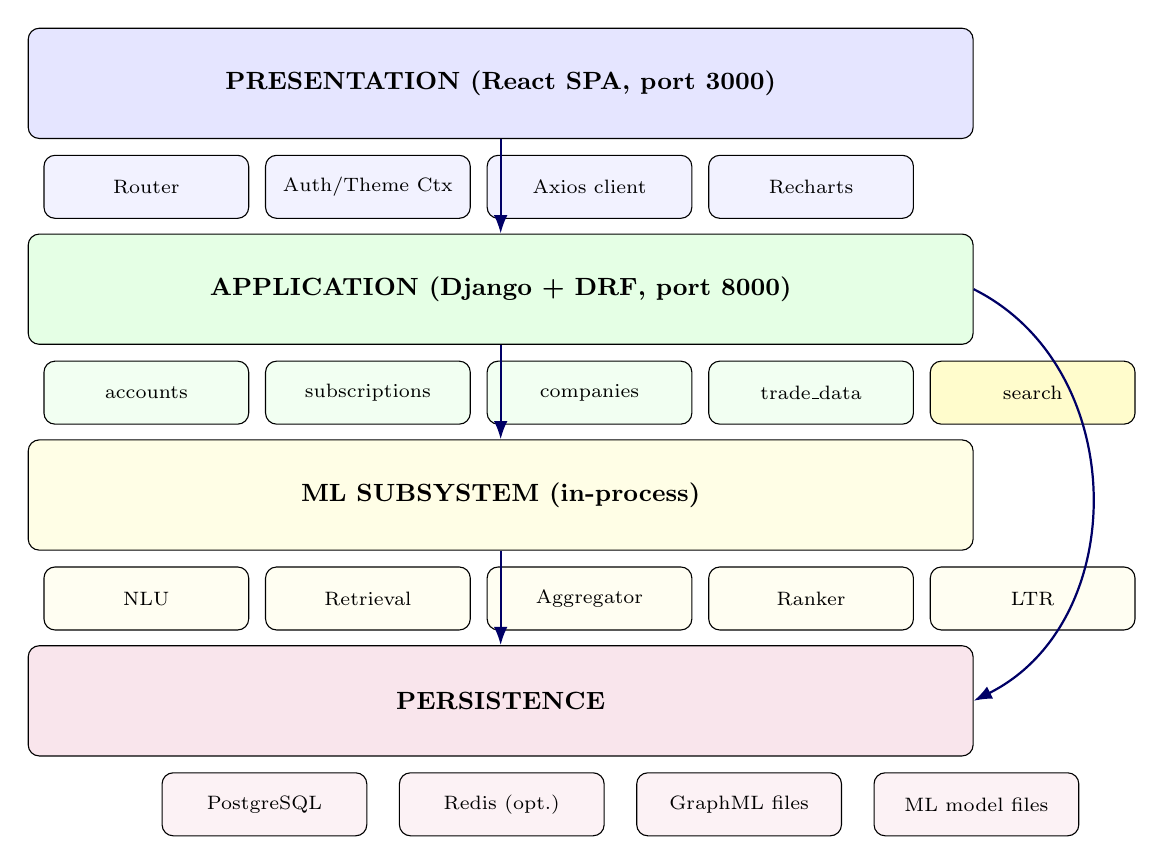
\begin{tikzpicture}[node distance=0.6cm,
    layer/.style={draw,rounded corners,minimum width=12cm,minimum height=1.4cm,align=center,font=\small\bfseries},
    sub/.style={draw,rounded corners,minimum width=2.6cm,minimum height=0.8cm,align=center,font=\scriptsize},
    arrow/.style={-Latex,thick,color=blue!40!black}]
  \node[layer,fill=blue!10] (pres) {PRESENTATION (React SPA, port 3000)};
  \node[sub,below=0.2cm of pres,xshift=-4.5cm,fill=blue!5] (router) {Router};
  \node[sub,right=0.2cm of router,fill=blue!5] (ctx) {Auth/Theme Ctx};
  \node[sub,right=0.2cm of ctx,fill=blue!5] (axios) {Axios client};
  \node[sub,right=0.2cm of axios,fill=blue!5] (charts) {Recharts};
  \node[layer,fill=green!10,below=1.2cm of pres] (app) {APPLICATION (Django + DRF, port 8000)};
  \node[sub,below=0.2cm of app,xshift=-4.5cm,fill=green!5] (auth) {accounts};
  \node[sub,right=0.2cm of auth,fill=green!5] (subs) {subscriptions};
  \node[sub,right=0.2cm of subs,fill=green!5] (cmp) {companies};
  \node[sub,right=0.2cm of cmp,fill=green!5] (td) {trade\_data};
  \node[sub,right=0.2cm of td,fill=yellow!20] (sr) {search};
  \node[layer,fill=yellow!10,below=1.2cm of app] (ml) {ML SUBSYSTEM (in-process)};
  \node[sub,below=0.2cm of ml,xshift=-4.5cm,fill=yellow!5] (nlu) {NLU};
  \node[sub,right=0.2cm of nlu,fill=yellow!5] (retr) {Retrieval};
  \node[sub,right=0.2cm of retr,fill=yellow!5] (agg) {Aggregator};
  \node[sub,right=0.2cm of agg,fill=yellow!5] (rank) {Ranker};
  \node[sub,right=0.2cm of rank,fill=yellow!5] (ltr) {LTR};
  \node[layer,fill=purple!10,below=1.2cm of ml] (pers) {PERSISTENCE};
  \node[sub,below=0.2cm of pers,xshift=-3cm,fill=purple!5] (pg) {PostgreSQL};
  \node[sub,right=0.4cm of pg,fill=purple!5] (rd) {Redis (opt.)};
  \node[sub,right=0.4cm of rd,fill=purple!5] (gm) {GraphML files};
  \node[sub,right=0.4cm of gm,fill=purple!5] (mod) {ML model files};
  \draw[arrow] (pres) -- (app);
  \draw[arrow] (app) -- (ml);
  \draw[arrow] (ml) -- (pers);
  \draw[arrow] (app.east) .. controls +(2,-1) and +(2,1) .. (pers.east);
\end{tikzpicture}
\caption{Layered Zarailink architecture.}
\label{fig:layered}
\end{figure}

\section{Tracing a search request end-to-end}
\label{sec:trace}

This is the single best way to internalise the architecture: walk through
what happens when a user submits a search query.

\begin{exampleBox}
\textbf{Scenario.} A logged-in user types
\emph{``cheap basmati rice from Punjab to UAE under \$0.40/kg''} into the
search bar and presses Enter.
\end{exampleBox}

\begin{enumerate}
  \item \textbf{[Browser]} \fileref{frontend/src/components/Search/SearchHome.js}
        captures the keystroke, calls \inlinecode{searchService.search(query)}.
  \item \textbf{[Browser → Network]} Axios issues
        \inlinecode{POST http://localhost:8000/api/search/} with body
        \inlinecode{\{"q": "cheap basmati ..."\}} and the session cookie
        attached (\inlinecode{withCredentials: true} from
        \fileref{frontend/src/services/api.js}).
  \item \textbf{[Django middleware]} The request flows through the
        middleware stack listed in \fileref{settings.py:65--75}: Security
        $\rightarrow$ Session $\rightarrow$ CORS $\rightarrow$ Common
        $\rightarrow$ CSRF $\rightarrow$ Auth $\rightarrow$ Messages
        $\rightarrow$ Clickjacking $\rightarrow$ Auditlog. The user object
        gets attached to \inlinecode{request.user} during the Auth step.
  \item \textbf{[URL resolver]} \fileref{backend/zarailink/urls.py:33}
        forwards \inlinecode{api/search/} to \fileref{backend/search/urls.py}.
  \item \textbf{[ViewSet]} The matching DRF action in
        \fileref{backend/search/views.py} runs.
  \item \textbf{[SearchService]} The view delegates to
        \fileref{backend/search/services/search\_service.py:SearchService}.
        This is the orchestrator.
  \item \textbf{[Stage 1 --- NLU]} \inlinecode{ModernNLUEngine.parse(query)}
        runs in \fileref{nlu_engine.py}:
    \begin{enumerate}
      \item \textbf{Cache check} (Redis or LocMem). MD5 hash of the
            query; on hit, return cached structured intent.
      \item \textbf{Intent classification} via SetFit (\inlinecode{BUY} vs
            \inlinecode{SELL}) using the model in
            \fileref{backend/models/zarai_intent_model/}.
      \item \textbf{Entity extraction} via GLiNER --- pulls country names,
            product mentions, quantities, price operators in one pass.
      \item \textbf{Keyword isolation} via KeyBERT --- strips ``urgently
            looking for'', ``please send quotation'', etc.
      \item \textbf{Geographic resolution} via RapidFuzz --- normalises
            ``Pak'' $\to$ ``Pakistan'', ``UAE'' $\to$ ``United Arab Emirates''.
      \item \textbf{Price logic} via regex first, falling back to
            OpenRouter LLM only if regex extraction fails. The result is a
            structured dict like:
        \begin{lstlisting}[language=Python,caption={Example NLU output},numbers=none]
{
  "action": "BUY",
  "products": ["basmati rice"],
  "from_country": "Pakistan",
  "to_country": "United Arab Emirates",
  "price_op": "<=",
  "price_value": 0.40,
  "price_currency": "USD",
  "price_unit": "kg",
  "raw_query": "cheap basmati rice from Punjab to UAE under $0.40/kg"
}
        \end{lstlisting}
    \end{enumerate}
  \item \textbf{[Stage 2 --- Candidate retrieval]}
        \fileref{backend/search/services/candidate\_retrieval.py} maps the
        product list to a set of \inlinecode{ProductSubCategory} IDs by:
    \begin{itemize}
      \item Loading \fileref{backend/search\_index.pkl} (in-memory).
      \item Running BM25 over product names.
      \item Running cosine similarity against the SentenceTransformer
            embeddings (\fileref{vector_store.py}).
      \item Running RapidFuzz fuzzy match for typos.
      \item Merging the three rankings.
    \end{itemize}
  \item \textbf{[Stage 3 --- Aggregation]}
        \fileref{backend/search/services/aggregation.py:SupplierAggregator}
        runs a single Postgres query (the heaviest in the pipeline) that:
    \begin{itemize}
      \item Filters \inlinecode{Transaction} rows by product subcategory,
            from-country, to-country, and price range.
      \item Groups by supplier company.
      \item Computes \inlinecode{SUM(volume)},
            \inlinecode{AVG(price)} (volume-weighted), \inlinecode{COUNT}
            (shipment frequency), \inlinecode{MAX(date)} (recency), and
            buyer-concentration metrics.
    \end{itemize}
  \item \textbf{[Stage 4 --- Ranking]}
        \fileref{backend/search/services/ranking\_ltr.py:RankingEnsemble}
        scores each candidate. The ensemble is:
        \[
        \text{score}_i = 0.7\,\text{heuristic}(i) + 0.3\,\text{LightGBM}(i)
        \]
        The heuristic side uses min-max-scaled volume, recency,
        frequency, price-fit; the LightGBM side runs the LambdaRank model
        from \fileref{backend/search/models/lgbm_ltr.txt}.
  \item \textbf{[Response]} The view serialises a list of supplier dicts
        and returns JSON over HTTPS.
  \item \textbf{[Browser]} \fileref{SearchResults.js} renders the list,
        wires up filters, sort, pagination, and clicking a result navigates
        to \fileref{DealDetail.js}.
\end{enumerate}

\begin{whyBox}
\textbf{Why a four-stage pipeline?} Each stage has a different cost model:
NLU is cheap and cacheable, retrieval is moderately heavy but bounded,
aggregation hits PostgreSQL, ranking is in-memory math. Splitting the
pipeline lets the team \emph{cache aggressively at the cheap end} and
parallelise / scale the expensive end independently. It also lets
unit-tests target one stage at a time --- a virtue you will appreciate when
debugging a search miss.
\end{whyBox}

\section{Authentication and authorisation flow}

Zarailink uses Django's built-in session-cookie auth. The flow:

\begin{enumerate}
  \item \textbf{Signup} (\fileref{POST /accounts/api/signup/}). Body
        contains \inlinecode{name, email, password, country}. The view
        constructs a \inlinecode{UserRegisterForm}, saves the user, marks
        \inlinecode{is_active = True} and \inlinecode{email_verified = True}
        immediately (the form's \inlinecode{is_active=False} is overridden).
  \item \textbf{Login} (\fileref{POST /accounts/api/login/}). The view
        calls Django's \inlinecode{authenticate(...)} then
        \inlinecode{login(request, user)} which writes a session cookie
        named \inlinecode{sessionid}.
  \item \textbf{Subsequent requests.} The browser includes the
        \inlinecode{sessionid} cookie (axios is configured with
        \inlinecode{withCredentials: true}). On the server,
        \inlinecode{SessionMiddleware} loads the session, then
        \inlinecode{AuthenticationMiddleware} attaches
        \inlinecode{request.user}.
  \item \textbf{Permission check.} Each protected view starts with
        \inlinecode{if not request.user.is_authenticated: return 401}.
        DRF \inlinecode{ViewSet}s use \inlinecode{permission_classes} on
        the class.
  \item \textbf{Logout} (\fileref{POST /accounts/api/logout/}). The view
        calls \inlinecode{logout(request)} which destroys the session.
\end{enumerate}

\begin{noviceBox}
\textbf{Why session-based and not JWT?} JWTs are stateless --- the server
needs no DB lookup to validate them. That is great for horizontally
scaled, polyglot back ends. Sessions, by contrast, are simpler to revoke
(just delete the row) and avoid the perennial JWT footguns (expiry, refresh
tokens, key rotation). For a Django monolith with a single backend, the
session model is plainly easier. The presence of
\inlinecode{djangorestframework-simplejwt} in
\fileref{requirements.txt} is a leftover; nothing in the codebase wires it
up.
\end{noviceBox}

\section{The token-balance economy}

A core product mechanic: every user has a \inlinecode{token_balance}
(integer, default 0; \fileref{accounts/models.py:48}). To unlock a
\textbf{key contact's} phone or email, the user spends one token. The
ledger row is a \inlinecode{KeyContactUnlock}
(\fileref{companies/models.py:167}).

The token economy is sustained by:

\begin{itemize}
  \item \textbf{Subscription plans} (\fileref{subscriptions/models.py:SubscriptionPlan})
        --- monthly token grants.
  \item \textbf{Redeem codes} (\fileref{subscriptions/models.py:RedeemCode})
        --- one-shot bundles purchased from the team.
  \item \textbf{Token purchases} (\fileref{subscriptions/models.py:TokenPurchase})
        --- direct top-ups.
  \item \textbf{Admin grants} --- Django admin actions
        (\fileref{accounts/admin.py:add_100_tokens, add_1000_tokens})
        for support cases.
\end{itemize}

The authority for ``does this user have access?'' is in
\fileref{backend/subscriptions/services.py:get_access_state} and
\fileref{purchase_access}. A view that wants to gate a feature behind
tokens calls these helpers; they encapsulate the ``check balance, deduct,
record audit log'' transaction in one place so feature views stay clean.

\section{Caching strategy}

\begin{itemize}
  \item \textbf{NLU cache.} The structured intent dict for a query is
        keyed by MD5 hash of the lowercased, stripped query. TTL: 24
        hours. On a Redis-backed deploy this is shared across worker
        processes; on LocMem it is per-process. See
        \fileref{nlu_engine.py} (cache hooks).
  \item \textbf{Search-index pickle.} The product subcategory $\to$ id
        lookup, BM25 index, and embedding matrix are all serialised into
        a single \fileref{backend/search\_index.pkl} loaded once at boot.
  \item \textbf{Django ORM `select\_related` / `prefetch\_related`.} Hot
        endpoints (e.g.~\fileref{search/views.py:supplier\_detail}) batch
        the foreign-key joins to avoid N+1 queries.
  \item \textbf{Redis Insight UI.} The team can inspect cache contents
        live at \url{http://localhost:8001} when the
        \inlinecode{redis-stack} container is running.
\end{itemize}

\section{Data flow at a glance}

Figure~\ref{fig:dataflow} traces the data lineage from the original Excel
files all the way to a search result.

\begin{figure}[h]
\centering
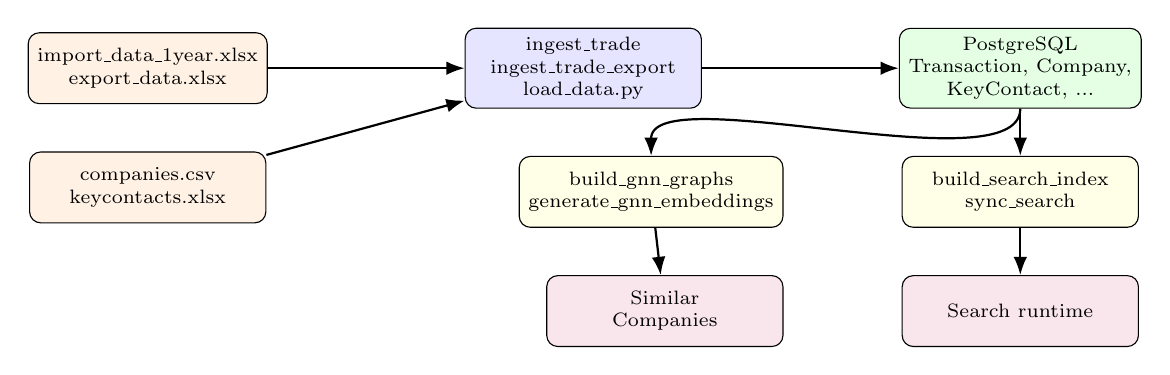
\begin{tikzpicture}[node distance=0.6cm and 1.5cm,
    box/.style={draw,rounded corners,minimum width=3cm,minimum height=0.9cm,align=center,font=\scriptsize},
    arrow/.style={-Latex,thick}]
  \node[box,fill=orange!10] (xls) {import\_data\_1year.xlsx\\export\_data.xlsx};
  \node[box,fill=orange!10,below=of xls] (csv) {companies.csv\\keycontacts.xlsx};
  \node[box,fill=blue!10,right=2.5cm of xls] (ingest) {ingest\_trade\\ingest\_trade\_export\\ load\_data.py};
  \node[box,fill=green!10,right=2.5cm of ingest] (db) {PostgreSQL\\Transaction, Company,\\KeyContact, ...};
  \node[box,fill=yellow!10,below=of db] (idx) {build\_search\_index\\sync\_search};
  \node[box,fill=yellow!10,left=of idx] (gnn) {build\_gnn\_graphs\\generate\_gnn\_embeddings};
  \node[box,fill=purple!10,below=of idx] (search) {Search runtime};
  \node[box,fill=purple!10,left=of search] (sim) {Similar\\Companies};
  \draw[arrow] (xls) -- (ingest);
  \draw[arrow] (csv) -- (ingest);
  \draw[arrow] (ingest) -- (db);
  \draw[arrow] (db) -- (idx);
  \draw[arrow] (db.south) .. controls +(0,-1) and +(0,1) .. (gnn.north);
  \draw[arrow] (idx) -- (search);
  \draw[arrow] (gnn) -- (sim);
\end{tikzpicture}
\caption{From Excel to search results: the data pipeline.}
\label{fig:dataflow}
\end{figure}

\section{The middleware stack, line by line}

The order of \fileref{settings.py:65--75} matters; here is what each layer
does and why it is at that position:

\begin{enumerate}
  \item \textbf{SecurityMiddleware} --- HTTPS redirects, HSTS headers,
        XSS filter. Must be early so it can short-circuit insecure
        requests.
  \item \textbf{SessionMiddleware} --- loads the session from the
        \inlinecode{sessionid} cookie. Must precede
        \inlinecode{AuthenticationMiddleware}.
  \item \textbf{CorsMiddleware} --- adds CORS headers. Django's docs
        require it before \inlinecode{CommonMiddleware} so that CORS
        responses are emitted even when Common slash-redirects.
  \item \textbf{CommonMiddleware} --- URL normalisation, ETag handling.
  \item \textbf{CsrfViewMiddleware} --- enforces CSRF tokens on unsafe
        methods. Must run before view dispatch.
  \item \textbf{AuthenticationMiddleware} --- attaches
        \inlinecode{request.user}.
  \item \textbf{MessageMiddleware} --- the Django flash-message system.
  \item \textbf{XFrameOptionsMiddleware} --- sets
        \inlinecode{X-Frame-Options: DENY}.
  \item \textbf{AuditlogMiddleware} --- pulls the user from the request
        and stores it on a thread-local so model-save signals can record
        ``who made this change''.
\end{enumerate}

\section{Testing pyramid (preview)}

The repo ships an extensive \fileref{conftest.py} with 28 reusable
fixtures (users, companies, plans, redeem codes, contacts, etc.) plus
\fileref{pytest.ini}. Tests live in:

\begin{itemize}
  \item \fileref{backend/accounts/tests/} --- model + view tests.
  \item \fileref{backend/companies/tests/test\_views.py}.
  \item \fileref{backend/subscriptions/tests/test\_views.py}.
  \item \fileref{backend/search/tests/test\_scope\_consistency.py}.
  \item Several loose \inlinecode{test\_*.py} files in
        \fileref{backend/} root used as ad-hoc reliability harnesses
        (\fileref{reliability\_test.py}, \fileref{perf\_test.py},
        \fileref{diagnose\_typo\_queries.py}, etc.).
\end{itemize}

We dedicate Chapter~\ref{ch:testing} to the test suite.

\section{Where things live (the cheat sheet)}

\begin{table}[h]
\centering
\small
\begin{tabular}{p{4.5cm} p{9cm}}
\toprule
\textbf{If you want to change\dots} & \textbf{Open\dots} \\
\midrule
A backend URL                       & \fileref{backend/<app>/urls.py} \\
A backend endpoint's behaviour      & \fileref{backend/<app>/views.py} \\
A database field                    & \fileref{backend/<app>/models.py} (then \inlinecode{makemigrations}) \\
The search ranking weights          & \fileref{backend/search/services/ranking.py} \\
The NLU intent labels               & \fileref{backend/search/services/nlu_engine.py} \\
A search-result React component     & \fileref{frontend/src/components/Search/} \\
The auth context state              & \fileref{frontend/src/context/AuthContext.js} \\
Tailwind theme                      & \fileref{frontend/tailwind.config.js} \\
Subscription plans                  & \fileref{backend/subscriptions/management/commands/create_plans.py} \\
\bottomrule
\end{tabular}
\caption{One-line ``where do I edit this'' lookup.}
\label{tab:cheat}
\end{table}
% ===== end chapters/03_architecture.tex =====

% ===== inlined from chapters/04_backend.tex =====
\chapter{Backend Deep Dive}
\label{ch:backend}

This chapter dissects every Django app and every endpoint in the backend.
We assume you have skim-read Chapter~\ref{ch:arch}; here we zoom in.

The backend is rooted at \fileref{backend/} and contains the project package
\fileref{backend/zarailink/} plus seven application packages. We cover
each in order.

\section{The project package: \texttt{zarailink/}}

Five files: \fileref{__init__.py} (empty), \fileref{settings.py} (392 lines),
\fileref{urls.py} (37 lines), \fileref{wsgi.py} and \fileref{asgi.py}.

\subsection{\texttt{settings.py}}
\label{sec:settings}

This is the single source of truth for runtime configuration.

\paragraph{Path \& env loading} (lines 13--21):

\begin{lstlisting}[language=Python,firstnumber=13]
from pathlib import Path
import os
from dotenv import load_dotenv
BASE_DIR = Path(__file__).resolve().parent.parent  # /backend
load_dotenv(BASE_DIR / '.env')
\end{lstlisting}

\inlinecode{BASE_DIR} resolves to \fileref{backend/} because
\fileref{settings.py} sits one level deep inside \fileref{zarailink/} and
\inlinecode{.parent.parent} walks up twice. The \inlinecode{load_dotenv}
call happens before any setting is read, so anything in \fileref{.env}
becomes available via \inlinecode{os.getenv}.

\paragraph{Secrets} (lines 28--30, 146):

\begin{lstlisting}[language=Python,numbers=none]
SECRET_KEY         = os.getenv('SECRET_KEY', '')
OPENROUTER_API_KEY = os.getenv('OPENROUTER_API_KEY', '')
OPENAI_API_KEY     = os.getenv('OPENAI_KEY', '')   # NOTE: the env var is OPENAI_KEY
\end{lstlisting}

\begin{warnBox}
\inlinecode{OPENAI_KEY} (no \inlinecode{API}) is the env var, but the
Python attribute is \inlinecode{OPENAI_API_KEY}. Mismatching these is a
common bug.
\end{warnBox}

\paragraph{Debug \& hosts} (lines 34--36):

\begin{lstlisting}[language=Python,numbers=none]
DEBUG = True
ALLOWED_HOSTS = ['localhost', '127.0.0.1', '.ngrok-free.dev', '.ngrok-free.app']
\end{lstlisting}

\inlinecode{DEBUG = True} is hard-coded; for production you must change
this manually.

\paragraph{INSTALLED\_APPS} (lines 41--63):

\begin{lstlisting}[language=Python,firstnumber=41]
INSTALLED_APPS = [
    'django.contrib.admin',
    'django.contrib.auth',
    'django.contrib.contenttypes',
    'django.contrib.sessions',
    'django.contrib.messages',
    'django.contrib.staticfiles',
    'rest_framework',
    'corsheaders',
    'django_ckeditor_5',
    'auditlog',
    'accounts',
    'subscriptions',
    'companies',
    'trade_data',
    'search',
    'django.contrib.postgres',
    'django_extensions',
]
\end{lstlisting}

Notably absent: the empty \inlinecode{home} and \inlinecode{trade_directory}
apps. Their directories exist but they are not installed.

\paragraph{Middleware order} (lines 65--75):

\begin{lstlisting}[language=Python,firstnumber=65]
MIDDLEWARE = [
    'django.middleware.security.SecurityMiddleware',
    'django.contrib.sessions.middleware.SessionMiddleware',
    'corsheaders.middleware.CorsMiddleware',
    'django.middleware.common.CommonMiddleware',
    'django.middleware.csrf.CsrfViewMiddleware',
    'django.contrib.auth.middleware.AuthenticationMiddleware',
    'django.contrib.messages.middleware.MessageMiddleware',
    'django.middleware.clickjacking.XFrameOptionsMiddleware',
    'auditlog.middleware.AuditlogMiddleware',
]
\end{lstlisting}

\paragraph{Templates} (lines 79--92): the project searches three template
roots: \fileref{backend/templates/}, \fileref{backend/accounts/templates/},
and \fileref{frontend/build/} (the React production build's
\fileref{index.html}). The catch-all URL at the end of
\fileref{urls.py:36} renders that file for any non-API URL --- this is
how the SPA gets shipped.

\paragraph{Database} (lines 100--109):

\begin{lstlisting}[language=Python,firstnumber=100]
DATABASES = {
    'default': {
        'ENGINE': 'django.db.backends.postgresql',
        'NAME': 'zarailink',
        'USER': 'postgres',
        'PASSWORD': 'postgres',
        'HOST': 'localhost',
        'PORT': '5432',
    }
}
\end{lstlisting}

\paragraph{Redis auto-detect} (lines 113--143). The pattern is:

\begin{lstlisting}[language=Python,firstnumber=115]
def is_redis_available():
    try:
        sock = socket.socket(socket.AF_INET, socket.SOCK_STREAM)
        sock.settimeout(1)
        result = sock.connect_ex(('127.0.0.1', 6379))
        sock.close()
        return result == 0
    except:
        return False
\end{lstlisting}

If the TCP probe succeeds, Django uses \inlinecode{django_redis.cache.RedisCache}
on \inlinecode{redis://127.0.0.1:6379/0}; otherwise it falls back to
\inlinecode{django.core.cache.backends.locmem.LocMemCache}.

\paragraph{Logging} (lines 149--187): two formatters
(\inlinecode{verbose}, \inlinecode{simple}), two handlers
(\inlinecode{console} at DEBUG, \inlinecode{file} at ERROR writing to
\fileref{backend/debug.log}), two named loggers (\inlinecode{django} at
INFO, \inlinecode{zarailink} at DEBUG).

\paragraph{Auth wiring}:
\begin{itemize}
  \item \fileref{settings.py:209} \inlinecode{AUTH_USER_MODEL = 'accounts.User'}.
  \item \fileref{settings.py:212} \inlinecode{LOGIN_REDIRECT_URL = '/dashboard'}.
  \item \fileref{settings.py:213} \inlinecode{LOGOUT_REDIRECT_URL = '/login'}.
\end{itemize}

\paragraph{CORS} (lines 336--369): localhost on ports 3000/3001/4000 are
explicitly whitelisted, plus a regex allowing any
\inlinecode{http://localhost:<port>}. \inlinecode{CORS_ALLOW_CREDENTIALS = True}
is essential for cookie-based auth to flow cross-origin.

\paragraph{Session security} (lines 372--391):

\begin{lstlisting}[language=Python,firstnumber=372]
CSRF_TRUSTED_ORIGINS    = [...same localhost list...]
CSRF_COOKIE_HTTPONLY    = False  # JS must read it for X-CSRFToken header
CSRF_COOKIE_SAMESITE    = 'Lax'
SESSION_COOKIE_SAMESITE = 'Lax'
SESSION_COOKIE_HTTPONLY = True
SESSION_COOKIE_SECURE   = False  # dev only
SECURE_CONTENT_TYPE_NOSNIFF = True
SECURE_BROWSER_XSS_FILTER   = True
X_FRAME_OPTIONS         = 'DENY'
SESSION_COOKIE_AGE      = 1209600   # 14 days
SESSION_SAVE_EVERY_REQUEST   = True
SESSION_EXPIRE_AT_BROWSER_CLOSE = False
\end{lstlisting}

\subsection{\texttt{urls.py}}

The URL root mounts each app at a stable prefix:

\begin{lstlisting}[language=Python,firstnumber=26]
urlpatterns = [
    path('favicon.ico', favicon),
    path('admin/', admin.site.urls),
    path('accounts/', include('accounts.urls')),
    path('api/subscriptions/', include('subscriptions.urls')),
    path('api/', include('companies.urls')),    # mounted at /api/, not /api/companies/
    path('api/search/', include('search.urls')),
    path("ckeditor5/", include('django_ckeditor_5.urls')),
    path('api-auth/', include('rest_framework.urls')),
    re_path(r'^.*$', TemplateView.as_view(template_name='index.html')),
]
\end{lstlisting}

\begin{warnBox}
The \inlinecode{re_path(r'\^.\*\$', ...)} catch-all is the React SPA
fallback. It must remain \emph{last}, otherwise it will swallow API
routes.
\end{warnBox}

\subsection{\texttt{wsgi.py} and \texttt{asgi.py}}

Both are stock Django bootstraps that set
\inlinecode{DJANGO_SETTINGS_MODULE = 'zarailink.settings'} and call
\inlinecode{get_wsgi_application()} or \inlinecode{get_asgi_application()}
respectively. Use \fileref{wsgi.py} with gunicorn/uWSGI; use
\fileref{asgi.py} with Daphne/Uvicorn for async.

\section{App: \texttt{accounts}}
\label{sec:accounts}

The custom user model and the entire authentication API. App config:
\inlinecode{AccountsConfig} with \inlinecode{default_auto_field = BigAutoField}.

\subsection{The \texttt{User} model}

\fileref{backend/accounts/models.py} defines exactly two classes:
\inlinecode{CustomUserManager} (lines 9--35) and \inlinecode{User} (lines
38--105).

The manager swaps Django's \inlinecode{username} for \inlinecode{email} as
the unique identifier:

\begin{lstlisting}[language=Python,firstnumber=14]
def create_user(self, email, password=None, username=None, **extra_fields):
    if not email:
        raise ValueError(_('The Email must be set'))
    email = self.normalize_email(email)
    user  = self.model(email=email, username=username, **extra_fields)
    user.set_password(password)
    user.save(using=self._db)
    return user
\end{lstlisting}

The \inlinecode{User} model adds these custom fields on top of
\inlinecode{AbstractUser}:

\begin{table}[h]
\centering
\small
\begin{tabular}{p{3.0cm} p{3.5cm} p{8cm}}
\toprule
\textbf{Field} & \textbf{Type} & \textbf{Options / purpose} \\
\midrule
\inlinecode{email} & \inlinecode{EmailField} & \inlinecode{unique=True} (used as login) \\
\inlinecode{username} & \inlinecode{CharField(150)} & nullable; demoted to optional \\
\inlinecode{bio} & \inlinecode{CharField(500)} & default empty string \\
\inlinecode{country} & \inlinecode{CharField(100)} & nullable \\
\inlinecode{email_verified} & \inlinecode{BooleanField} & default \inlinecode{False} \\
\inlinecode{verification_token} & \inlinecode{UUIDField} & \inlinecode{default=uuid.uuid4, unique=True} \\
\inlinecode{token_created_at} & \inlinecode{DateTimeField} & default \inlinecode{timezone.now} \\
\inlinecode{phone_number} & \inlinecode{CharField(30)} & nullable \\
\inlinecode{job_title} & \inlinecode{CharField(100)} & nullable \\
\inlinecode{token_balance} & \inlinecode{IntegerField} & default 0 (the token economy) \\
\bottomrule
\end{tabular}
\caption{\inlinecode{accounts.User} custom fields.}
\end{table}

\inlinecode{USERNAME_FIELD = "email"} (line 63) plus
\inlinecode{REQUIRED_FIELDS = ["first_name", "last_name"]} make the model
log-in via email and require first/last name on \inlinecode{createsuperuser}.

\paragraph{Methods worth memorising}:
\begin{itemize}
  \item \inlinecode{is_verification_token_valid()} --- returns
        \inlinecode{False} if already verified, otherwise compares
        \inlinecode{token_created_at + 24h} to \inlinecode{now()}. The
        24-hour expiry on email verification lives here.
  \item \inlinecode{regenerate_verification_token()} --- assigns a fresh
        UUID and resets \inlinecode{token_created_at} (used by the
        ``resend verification email'' endpoint).
  \item \inlinecode{has_tokens(amount=1)} --- boolean balance check.
  \item \inlinecode{deduct_tokens(amount=1)} --- atomic deduct, returns
        success bool.
  \item \inlinecode{add_tokens(amount)} --- credit. Returns \inlinecode{None}
        (no boolean).
\end{itemize}

\subsection{The audit log (\texttt{accounts/audit.py})}

\fileref{backend/accounts/audit.py} defines an \inlinecode{AuditLog}
model. \textbf{Caveat}: Django auto-discovers models inside
\fileref{models.py}; placing them in \fileref{audit.py} means no migration
is auto-generated. The file is currently \emph{infrastructure-in-waiting}:
the helpers \inlinecode{log_action(...)} and
\inlinecode{get_user_activity(...)} are imported by views but the table is
not created without a manual migration.

The third-party \inlinecode{auditlog} app (registered in
\fileref{INSTALLED_APPS}, configured at the bottom of
\fileref{companies/models.py}) is the live audit trail.

\subsection{Authentication API (every endpoint)}

\fileref{backend/accounts/views.py} contains 9 function-based views and one
HTML view. Mounted under \fileref{accounts/} via the project URLs. Below
is the complete table, then a per-endpoint walkthrough.

\begin{table}[h]
\centering
\small
\begin{tabular}{p{0.8cm} p{6.5cm} p{6.5cm}}
\toprule
\textbf{M.} & \textbf{URL} & \textbf{Purpose} \\
\midrule
GET/POST & \inlinecode{accounts/register/} & HTML form (Django template) \\
GET/POST & \inlinecode{accounts/login/} & Same view, alias \\
POST & \inlinecode{accounts/api/signup/} & JSON signup \\
POST & \inlinecode{accounts/api/login/} & JSON login (sets session cookie) \\
POST & \inlinecode{accounts/api/logout/} & Destroys session \\
GET  & \inlinecode{accounts/api/check-auth/} & Bootstrap session for SPA \\
POST & \inlinecode{accounts/api/forgot-password/} & Sends reset email \\
GET  & \inlinecode{accounts/api/verify-email/<uuid:token>/} & Verifies, redirects to React \\
POST & \inlinecode{accounts/api/resend-verification/} & Re-sends multi-part HTML+text email \\
POST & \inlinecode{accounts/api/update-profile/} & Auth-required \\
POST & \inlinecode{accounts/api/change-password/} & Auth-required, re-auths session \\
GET  & \inlinecode{accounts/password_reset_confirm/<uidb64>/<token>/} & Django's stock view \\
GET  & \inlinecode{accounts/password_reset_complete/} & Django's stock view \\
\bottomrule
\end{tabular}
\caption{\texttt{accounts} endpoints.}
\label{tab:accounts-endpoints}
\end{table}

\paragraph{POST \texttt{/accounts/api/signup/}} (lines 38--76).
Body: \inlinecode{\{name, email, password, country\}}. Internally
constructs a \inlinecode{UserRegisterForm}, but \emph{overrides} the form's
\inlinecode{is_active=False} by setting both \inlinecode{is_active = True}
and \inlinecode{email_verified = True} immediately.

\begin{whyBox}
The form was originally written for an email-verification flow; the team
short-circuited it for the demo so users can sign up and use the product
right away. If you ever turn email verification back on, remove the
\inlinecode{user.email_verified = True} line and re-enable
\inlinecode{is_active = False}.
\end{whyBox}

\paragraph{POST \texttt{/accounts/api/login/}} (lines 79--105). Calls
\inlinecode{authenticate(request, email=..., password=...)} (which works
because \inlinecode{USERNAME_FIELD = 'email'}) then
\inlinecode{login(request, user)}. The session cookie is set by Django
automatically. The 200 response includes
\inlinecode{\{success, user: \{name, email, email_verified, token_balance\}\}}.

\paragraph{POST \texttt{/accounts/api/logout/}} (lines 108--111). Calls
\inlinecode{logout(request)} and returns \inlinecode{\{"success": true\}}.
No HTTP-method check.

\paragraph{GET \texttt{/accounts/api/check-auth/}} (lines 114--129). The
SPA calls this on page load. If \inlinecode{request.user.is_authenticated},
returns the same user payload as login; else
\inlinecode{\{"authenticated": false\}}.

\paragraph{POST \texttt{/accounts/api/forgot-password/}} (lines 132--157).
Body: \inlinecode{\{email\}}. Always returns
\inlinecode{\{"success": true\}} regardless of whether the email is
registered (anti-enumeration). On success, sends an email containing the
Django default token + base64-encoded UID, pointing back at
\inlinecode{accounts:password_reset_confirm}.

\paragraph{GET \texttt{/accounts/api/verify-email/<uuid:token>/}}
(lines 160--190). Looks up the user by token. Branches:
\begin{itemize}
  \item Already verified $\to$ redirects to
        \inlinecode{\{FRONTEND_URL\}/verify-email/\{token\}?status=already_verified}.
  \item Token expired ($> 24$h) $\to$ redirects with \inlinecode{?status=expired}.
  \item Token valid $\to$ marks verified \& active, redirects with
        \inlinecode{?status=verified}.
  \item Token not found $\to$ redirects with \inlinecode{?status=invalid}.
\end{itemize}

\paragraph{POST \texttt{/accounts/api/resend-verification/}}
(lines 193--313). Body: \inlinecode{\{email\}}. Re-rolls the verification
token, then composes a \emph{multi-part} email with both an HTML body
(branded green \inlinecode{\#1A4D2E}, ``Optimize Data. Empower Tomorrow.''
tagline) and a plain-text fallback. Anti-enumerates: if user not found,
still returns success.

\paragraph{POST \texttt{/accounts/api/update-profile/}} and
\paragraph{POST \texttt{/accounts/api/change-password/}} are
straightforward auth-gated mutations. The change-password view ends with
\inlinecode{update_session_auth_hash(request, user)}, which is the standard
Django incantation to keep the existing session valid after changing the
password (otherwise the user would be logged out instantly).

\subsection{Admin}

\inlinecode{UserAdmin(BaseUserAdmin)} (\fileref{accounts/admin.py:6--54})
exposes:
\begin{itemize}
  \item \inlinecode{list_display}: email, first/last name, email\_verified, token\_balance, is\_staff, date\_joined.
  \item \inlinecode{list_filter}: is\_staff, is\_superuser, email\_verified, date\_joined.
  \item \inlinecode{search_fields}: email, first/last name, phone\_number.
  \item Three custom actions: \inlinecode{add_100_tokens},
        \inlinecode{add_1000_tokens}, \inlinecode{verify_users} (bulk
        update to \inlinecode{email_verified = True}).
\end{itemize}

These actions are how customer-support style operations happen: a staff
user picks 200 accounts in the admin, hits \emph{Add 100 tokens to selected
users}, done.

\section{App: \texttt{companies}}
\label{sec:companies}

The company directory: who exists, what sector, what role, what products,
what key contacts.

\subsection{Models}

\fileref{backend/companies/models.py} defines seven model classes plus an
\inlinecode{auditlog} block:

\begin{itemize}
  \item \inlinecode{Sector}, \inlinecode{CompanyRole}, \inlinecode{CompanyType}
        --- three taxonomy tables. Each has \inlinecode{name +
        description}. Used by \inlinecode{Company} via \inlinecode{ForeignKey(SET_NULL)}.
  \item \inlinecode{Company} (lines 47--114) --- the directory entity. 24
        fields covering identity, location, contact info, business
        details, verification status, and bookkeeping. Two indexes:
        \inlinecode{('country', 'sector')} and \inlinecode{('verification_status',)}.
        Verification is a four-state choice:
        \inlinecode{unverified, pending, verified, premium}.
  \item \inlinecode{CompanyProduct} (lines 117--139) --- products a company
        offers. \inlinecode{ForeignKey(Company, CASCADE)},
        \inlinecode{name}, \inlinecode{description}, \inlinecode{variety}
        (e.g.~``Basmati'', ``Super Kernel''), \inlinecode{value_added}
        (e.g.~``Organic certified''), \inlinecode{hsn_code}.
  \item \inlinecode{KeyContact} (lines 142--164) --- a person at a company:
        \inlinecode{name, designation, phone, whatsapp, email, is_public}.
        \inlinecode{is_public=True} contacts are visible without spending
        a token.
  \item \inlinecode{KeyContactUnlock} (lines 167--191) --- the ``user X
        spent 1 token to see contact Y'' ledger.
        \inlinecode{unique_together=['user', 'key_contact']} prevents
        double-charging.
\end{itemize}

The auditlog block at the end registers \inlinecode{Company},
\inlinecode{CompanyProduct}, and \inlinecode{KeyContact}, so any change to
those models lands in the third-party \inlinecode{auditlog_logentry} table
with the user attribution that the middleware thread-local provides.

\subsection{Serializers}

\fileref{backend/companies/serializers.py} has eight serializers. The
clever one is \inlinecode{KeyContactSerializer} (lines 39--72) which
implements the paywall at the serialization layer:

\begin{lstlisting}[language=Python,firstnumber=60]
def to_representation(self, instance):
    rep = super().to_representation(instance)
    if not (instance.is_public or rep['is_unlocked']):
        rep['phone'] = rep['email'] = rep['whatsapp'] = "Locked"
    return rep
\end{lstlisting}

If neither public nor unlocked-by-this-user, the contact fields are
overwritten with the literal string \inlinecode{Locked} (with a lock emoji
in the source). The frontend reads this string and renders the lock icon
plus an ``Unlock for 1 token'' button.

\subsection{Endpoints (\texttt{companies/views.py})}

Mounted at \inlinecode{/api/} (so \inlinecode{companies/} becomes
\inlinecode{/api/companies/}, and so on).

\begin{table}[h]
\centering
\small
\begin{tabular}{p{0.8cm} p{6.5cm} p{6.5cm}}
\toprule
\textbf{M.} & \textbf{URL} & \textbf{What it does} \\
\midrule
GET  & \inlinecode{/api/companies/} & List+filter directory; supports \inlinecode{?search=, ?use_ai=, ?region=, ?sector=, ?type=, ?role=, ?country=}. \\
GET  & \inlinecode{/api/companies/<pk>/} & Detail, with nested products + key contacts. \\
GET  & \inlinecode{/api/companies/regions/} & Distinct provinces. \\
GET  & \inlinecode{/api/companies/countries/} & Distinct countries; supports \inlinecode{?role=}. \\
GET  & \inlinecode{/api/companies/hsn_codes/} & Distinct HSN codes from \inlinecode{CompanyProduct}. \\
GET  & \inlinecode{/api/key-contacts/} & List contacts; \inlinecode{?company=}. \\
GET  & \inlinecode{/api/key-contacts/<pk>/} & Single contact (with paywall). \\
POST & \inlinecode{/api/key-contacts/<pk>/unlock/} & Spend 1 token; create \inlinecode{KeyContactUnlock}. \\
GET  & \inlinecode{/api/sectors/} & Sectors lookup. \\
GET  & \inlinecode{/api/company-types/} & Types lookup. \\
GET  & \inlinecode{/api/company-roles/} & Roles lookup. \\
\bottomrule
\end{tabular}
\caption{\texttt{companies} endpoints.}
\label{tab:companies-endpoints}
\end{table}

\paragraph{\texttt{CompanyViewSet.get\_queryset} --- the smart-search hook}
(\fileref{companies/views.py:61--167}). When you pass \inlinecode{?search=foo&use_ai=true},
the view:

\begin{enumerate}
  \item Snapshots the first 100 candidates as a \inlinecode{values()} dict.
  \item Calls \fileref{utils/ai_service.py:AIService.smart_search(search,
        candidates)} (a GPT-4o-mini wrapper).
  \item Filters to whatever IDs GPT returned, preserving GPT's ordering
        with a \inlinecode{Case/When/IntegerField} \inlinecode{order_by}.
  \item If GPT returns nothing or errors, sets \inlinecode{self._ai_fallback = True}
        and falls back to plain
        \inlinecode{Q(name__icontains=search) | Q(description__icontains=search)}.
        The list response then carries \inlinecode{ai_fallback: true} so
        the frontend can show ``AI search unavailable, results from
        keyword fallback.''
\end{enumerate}

\paragraph{\texttt{KeyContactViewSet.unlock} --- the token transaction}
(\fileref{companies/views.py:212--270}). Atomic, CSRF-exempt, auth-required:

\begin{enumerate}
  \item If the contact is already unlocked by this user $\to$
        \inlinecode{\{"status": "already_unlocked"\}}.
  \item If \inlinecode{contact.is_public} $\to$ create the unlock with
        \inlinecode{tokens_charged = 0}.
  \item If user has no tokens $\to$ HTTP 402 with current balance.
  \item Else \inlinecode{user.deduct_tokens(1)} and create the unlock; HTTP
        200 with \inlinecode{tokens_charged = 1} and the now-unlocked
        contact serialized with the request context (so the frontend sees
        the real fields, not \inlinecode{Locked}).
\end{enumerate}

\subsection{Admin}

Seven admin registrations. The most interesting:

\begin{itemize}
  \item \inlinecode{CompanyAdmin} uses a custom \inlinecode{CompanyAdminForm}
        that swaps the description field to \inlinecode{CKEditor5Widget}.
        Six fieldsets: Basic Information, Description, Contact Information,
        Business Details, Status \& Flags, Metadata.
  \item \inlinecode{KeyContactAdmin} adds a
        \inlinecode{KeyContactUnlockInline} table inline so you can see
        ``who unlocked this contact'' directly on the page. A custom
        \inlinecode{unlock_count} method counts the inline rows.
\end{itemize}

\subsection{Management commands}

Nine custom commands under
\fileref{backend/companies/management/commands/}:

\begin{table}[h]
\centering
\small
\begin{tabular}{p{4.5cm} p{9cm}}
\toprule
\textbf{Command} & \textbf{What it does} \\
\midrule
\inlinecode{seed_roles} & Creates 5 baseline roles: Buyer, Supplier, Distributor, Manufacturer, Service Provider. \\
\inlinecode{setup_company_roles} & Creates 3 binary roles: Buyers, Suppliers, Both. Bulk-assigns every roleless company to ``Both''. \\
\inlinecode{import_companies} & Reads \fileref{companies.xlsx}, walks rows, and \inlinecode{update_or_create}s a \inlinecode{Company} per row using a column-mapping dict. Wrapped in \inlinecode{transaction.atomic()}. \\
\inlinecode{debug_companies} & Diagnostic: prints counts, lists roles, simulates a viewset filter. No-op on data. \\
\inlinecode{merge_sectors} & One-shot: merges \inlinecode{Sector(id=3, 'Confectionary')} into \inlinecode{Sector(id=4, 'Confectionery')} and deletes the duplicate. \\
\inlinecode{fix_sectors_hsn} & Generalisation of the above plus auto-assigns a random plausible HSN code to any \inlinecode{CompanyProduct} that lacks one. \\
\inlinecode{fix_company_data} & Bulk-marks every company \inlinecode{verification_status='verified'} (a one-shot for the demo). \\
\inlinecode{analyze_companies} & For every company description, runs \fileref{utils/ai_service.py:analyze_sentiment} and stores ``Positive''/''Negative''/''Neutral'' in \inlinecode{market_sentiment}. \\
\inlinecode{generate_embeddings} & For each verified company, calls \fileref{utils/ai_service.py:get_embedding} (OpenAI \inlinecode{text-embedding-3-small}, 1536-d) and stores in \inlinecode{trade_data.CompanyEmbedding}. \\
\inlinecode{index_companies} & Builds an HNSW vector index in Redis (\inlinecode{idx:companies}) for Smart Search. \\
\bottomrule
\end{tabular}
\caption{\texttt{companies} management commands.}
\end{table}

\section{App: \texttt{subscriptions}}
\label{sec:subscriptions}

The token-balance economy: plans, redeem codes, purchases, and the
unified paywall service.

\subsection{Models}

Five model classes in \fileref{backend/subscriptions/models.py}:

\begin{itemize}
  \item \inlinecode{SubscriptionPlan} --- \inlinecode{plan_name, price,
        currency, tokens_included, description, features} (a JSONField for
        feature flags).
  \item \inlinecode{UserSubscription} --- the active subscription record.
        \inlinecode{ForeignKey(plan, PROTECT)} ensures you cannot delete a
        plan that still has subscribers.
  \item \inlinecode{TokenPurchase} --- one-off token top-up record with
        payment provider/reference fields (PayPal, Stripe, JazzCash, etc.).
  \item \inlinecode{RedeemCode} --- a 12-character alphanumeric code
        (with confusable characters \inlinecode{0/O/I/1} stripped) that
        can be redeemed by exactly one user. Methods:
        \inlinecode{generate_code(length=12)} and
        \inlinecode{redeem(user)}.
  \item \inlinecode{UserAccess} --- the entitlement ledger. Two tiers:
        \inlinecode{HS_CODE} (full category access, costs 5{,}000 tokens)
        and \inlinecode{PRODUCT} (single subcategory, 500 tokens).
        \inlinecode{UniqueConstraint(['user','hscode','subcat_id'])} prevents
        double-grants.
\end{itemize}

\subsection{The paywall service: \texttt{subscriptions/services.py}}

This module is the \emph{single backend authority} for ``does this user
have access?'' Constants (lines 25--32):

\begin{lstlisting}[language=Python,firstnumber=25]
HS_CODE_PRICE  = 5000
PRODUCT_PRICE  = 500
FULL_ACCESS    = 'FULL_ACCESS'
PRODUCT_ACCESS = 'PRODUCT_ACCESS'
NO_ACCESS      = 'NO_ACCESS'
\end{lstlisting}

\paragraph{\texttt{get\_access\_state(user, hscode, subcat\_id=None)}}
(lines 35--60). Returns one of the three states. Logic:

\begin{enumerate}
  \item Anonymous $\to$ \inlinecode{NO_ACCESS}.
  \item Staff/superuser $\to$ \inlinecode{FULL_ACCESS} (admin bypass).
  \item Look up \inlinecode{UserAccess} rows for this user + this hscode.
  \item Any \inlinecode{HS_CODE} row $\to$ \inlinecode{FULL_ACCESS}.
  \item Else if \inlinecode{subcat_id} matches a \inlinecode{PRODUCT} row
        $\to$ \inlinecode{PRODUCT_ACCESS}.
  \item Else $\to$ \inlinecode{NO_ACCESS}.
\end{enumerate}

\paragraph{\texttt{purchase\_access(user, access\_type, hscode, subcat\_id=None)}}
(lines 63--108). Returns \inlinecode{(success: bool, message: str,
new_balance: Optional[int])}. Inside a \inlinecode{transaction.atomic()} it:

\begin{enumerate}
  \item Validates inputs and computes the price.
  \item \emph{Idempotency:} if the grant exists, returns
        \inlinecode{(True, "Access already granted.", balance)} without
        charging.
  \item Checks \inlinecode{token_balance >= price}; otherwise fails.
  \item Deducts and creates the \inlinecode{UserAccess}.
\end{enumerate}

\subsection{Endpoints}

\begin{table}[h]
\centering
\small
\begin{tabular}{p{0.8cm} p{6.5cm} p{6.5cm}}
\toprule
\textbf{M.} & \textbf{URL} & \textbf{Effect} \\
\midrule
GET  & \inlinecode{/api/subscriptions/plans/} & Lists all plans (no auth). \\
POST & \inlinecode{/api/subscriptions/redeem/} & ``Demo bypass'' --- credits the plan's tokens directly to \inlinecode{request.user.token_balance} (does not validate a real code). Auth required. \\
POST & \inlinecode{/api/subscriptions/purchase-access/} & Calls \inlinecode{services.purchase_access}. Auth required. \\
GET  & \inlinecode{/api/subscriptions/profile-data/} & Returns \inlinecode{\{entitlements, tokenHistory, telemetry\}} for the profile page. Auth required. \\
POST & \inlinecode{/api/subscriptions/generate-codes/} & Staff-only: bulk-creates 10 redeem codes for a given plan. Form-encoded. \\
\bottomrule
\end{tabular}
\caption{\texttt{subscriptions} endpoints.}
\label{tab:subs-endpoints}
\end{table}

\paragraph{\texttt{profile\_data\_view}} is rich enough to deserve a
walkthrough (\fileref{subscriptions/views.py:145--255}). It returns a
single payload that the React profile page renders into three tabs:

\begin{enumerate}
  \item \textbf{Entitlements.} For each \inlinecode{UserAccess} row,
        derives a name (\inlinecode{ProductCategory.hs_code} for
        HS\_CODE, \inlinecode{ProductSubCategory.id} for PRODUCT) and an
        \inlinecode{accessLevel} string.
  \item \textbf{Token history.} A union of three event streams:
        \inlinecode{UserAccess} (negative amount = spend),
        \inlinecode{TokenPurchase} (positive = top-up),
        \inlinecode{RedeemCode} (positive = redeem). Sorted descending by date.
  \item \textbf{Telemetry.} Two derived fields:
        \inlinecode{queries = total_tokens_spent // 10 + 12} and
        \inlinecode{productsViewed = total_tokens_spent // 50 + 5}.
        These are loose proxies (the real per-user query counter is not
        stored).
\end{enumerate}

\subsection{Admin}

Four admin classes; the highlight is \inlinecode{RedeemCodeAdmin} which
adds six bulk-generate actions, one per plan, each emoji-labelled.
Selecting the action seeds 15 fresh codes in one click. The status
badge column uses \inlinecode{format_html} to render coloured pills
(green/gray/red).

\subsection{Management commands}

\begin{itemize}
  \item \inlinecode{create_plans} --- seeds the six canonical plans (see
        Table~\ref{tab:plans}).
  \item \inlinecode{generate_codes} --- CLI alternative to the admin
        bulk action; resolves a plan by id or fuzzy name match, then
        generates a configurable number of codes.
\end{itemize}

\begin{table}[h]
\centering
\small
\begin{tabular}{p{4.5cm} r p{2cm} r}
\toprule
\textbf{Plan name} & \textbf{Price} & \textbf{Currency} & \textbf{Tokens} \\
\midrule
500 Credits           &    9.00 & PKR &    500 \\
5K Credits            &   32.00 & PKR &  5{,}000 \\
15K Credits           &   99.00 & PKR & 15{,}000 \\
6000 Credits Annually &   99.00 & PKR &  6{,}000 \\
60K Credits Annually  &  350.00 & PKR & 60{,}000 \\
900K Credits Annually & 1090.00 & PKR & 900{,}000 \\
\bottomrule
\end{tabular}
\caption{Subscription plans seeded by \texttt{create\_plans}.}
\label{tab:plans}
\end{table}

\section{App: \texttt{trade\_data}}
\label{sec:trade-data}

The most data-heavy app. Owns the trade product hierarchy and the
\inlinecode{Transaction} ledger, plus two embedding tables. Its
\fileref{views.py} and \fileref{admin.py} are intentionally empty --- this
is a model + management-command layer that other apps query directly.

\subsection{The product hierarchy}

A four-level tree on top of HS codes:

\begin{lstlisting}[caption={Product hierarchy},language=Python,numbers=none]
Product (HS chapter, e.g., 1701)
  -> ProductCategory (HS heading, e.g., 1701.99)
       -> ProductSubCategory (e.g., 1701.9990 "Refined Sugar")
            -> ProductItem (e.g., "White Refined Sugar 50KG Bag")
\end{lstlisting}

Each level is a Django model with a \inlinecode{ForeignKey(parent,
on_delete=CASCADE)}. The leaf, \inlinecode{ProductItem}, is what every
\inlinecode{Transaction} points at via a \inlinecode{ForeignKey(SET_NULL)}.

\subsection{The \texttt{Transaction} model}

The table that everything else is built on. 21 fields covering source,
direction, parties, geography, quantity, price, and bookkeeping. Key
fields (\fileref{trade_data/models.py:65--142}):

\begin{table}[h]
\centering
\small
\begin{tabular}{p{3.0cm} p{3.5cm} p{8cm}}
\toprule
\textbf{Field} & \textbf{Type} & \textbf{Notes} \\
\midrule
\inlinecode{trade_type} & \inlinecode{CharField, choices} & \inlinecode{IMPORT}/\inlinecode{EXPORT}, db-indexed. \\
\inlinecode{hs_code} & \inlinecode{CharField(50)} & db-indexed. \\
\inlinecode{product_item} & \inlinecode{ForeignKey(SET_NULL)} & to \inlinecode{ProductItem}. \\
\inlinecode{buyer/seller/shipping_agent} & \inlinecode{CharField(500)} & free-text. \\
\inlinecode{origin_country} & \inlinecode{CharField(100)} & db-indexed. \\
\inlinecode{destination_country} & \inlinecode{CharField(100)} & db-indexed. \\
\inlinecode{qty_kg/qty_mt} & \inlinecode{DecimalField(20,6)} & both kept; the ingest derives one from the other when one is missing. \\
\inlinecode{usd_per_kg/usd_per_mt} & \inlinecode{DecimalField(20,6)} & nullable. \\
\inlinecode{pkr/usd} & \inlinecode{DecimalField(30,2)} & total invoice value. \\
\inlinecode{reporting_date} & \inlinecode{DateField} & db-indexed for time queries. \\
\bottomrule
\end{tabular}
\caption{Highlights of the \inlinecode{Transaction} model.}
\end{table}

Seven indexes on \inlinecode{Meta.indexes} (lines 121--133) cover every hot
filter the search engine uses: \inlinecode{reporting_date, buyer, seller,
hs_code, trade_type, origin_country, destination_country}.

\begin{whyBox}
The model keeps both \emph{kg} and \emph{MT} (metric tonne) columns even
though one is just $1{,}000\times$ the other. Two reasons: (a)~the source
spreadsheets sometimes give one but not the other, and (b)~aggregation
queries like \inlinecode{SUM(qty_mt)} are cheaper to read than to compute
on the fly.
\end{whyBox}

\subsection{Embedding tables}

Two thin wrappers around vectors stored as JSON:

\begin{itemize}
  \item \inlinecode{CompanyEmbedding} ---
        \inlinecode{company_name} (unique), \inlinecode{embedding}
        (\inlinecode{JSONField}), \inlinecode{cluster_tag},
        \inlinecode{pagerank}, \inlinecode{degree}.
  \item \inlinecode{ProductEmbedding} ---
        \inlinecode{ForeignKey(ProductItem)} (unique), \inlinecode{embedding},
        \inlinecode{cluster_tag}.
\end{itemize}

These are populated by \inlinecode{generate_embeddings} (companies) and
\inlinecode{generate_gnn_embeddings} (referenced from the setup script).

\subsection{Ingestion commands}

\begin{itemize}
  \item \inlinecode{ingest_trade --file <xlsx>} --- IMPORT direction. Reads
        the Excel header at row 6 (so spreadsheet skipping happens
        automatically), normalises column names, formats HS codes to
        4-decimal strings, walks the product hierarchy with
        \inlinecode{get_or_create}, and bulk-inserts \inlinecode{Transaction}
        rows with \inlinecode{ignore_conflicts=True}.
  \item \inlinecode{ingest_trade_export --file <xlsx>} --- EXPORT direction;
        identical except \inlinecode{origin_country = "Pakistan"}.
  \item \inlinecode{repair_trade_companies} --- backfills the
        \inlinecode{Company} table from existing \inlinecode{Transaction}
        rows. Iterates with \inlinecode{.iterator()} to avoid loading all
        into memory; \inlinecode{get_or_create}s a directory entry per
        unique buyer/seller name.
\end{itemize}

\section{App: \texttt{search} (API surface)}
\label{sec:search-api}

We cover the heavy ML inside this app in Chapter~\ref{ch:search-engine}.
Here we focus on the API surface (\fileref{apps.py},
\fileref{models.py}, \fileref{urls.py}, \fileref{views.py}, the
management commands).

\subsection{Boot warmup (\texttt{search/apps.py})}

\fileref{search/apps.py} contains a small but important
\inlinecode{ready()} hook:

\begin{lstlisting}[language=Python,caption={NLU warmup}]
class SearchConfig(AppConfig):
    default_auto_field = 'django.db.models.BigAutoField'
    name = 'search'
    def ready(self):
        def _warmup():
            try:
                from .services.nlu_engine import ModernNLUEngine
                engine = ModernNLUEngine()
                engine.parse("buy sugar")
                engine.parse("sell wheat to UAE")
                print("[ZaraiLink] NLU warmup complete - system ready.")
            except Exception as e:
                print(f"[ZaraiLink] Warmup skipped: {e}")
        threading.Thread(target=_warmup, daemon=True).start()
\end{lstlisting}

When Django boots, a daemon thread runs two throwaway NLU parses. That
loads SetFit, GLiNER, and the SentenceTransformer once, so the first user
query does not eat a 5-second cold-start.

\subsection{The viewset and its endpoints}

\fileref{backend/search/views.py} (892 lines) is built around a single
\inlinecode{SearchViewSet(viewsets.ViewSet)} with
\inlinecode{permission_classes = [AllowAny]}. A module-level
singleton-pattern initialises the heavy \inlinecode{SearchService} once at
import time:

\begin{lstlisting}[language=Python,caption={Singleton SearchService}]
logger.info("Initializing Global SearchService on Startup...")
global_search_service = SearchService()
\end{lstlisting}

Every viewset instance reuses the same \inlinecode{SearchService}.

\begin{table}[h]
\centering
\small
\begin{tabular}{p{0.8cm} p{6.5cm} p{6.5cm}}
\toprule
\textbf{M.} & \textbf{URL} & \textbf{Action} \\
\midrule
GET & \inlinecode{/api/search/} & main NL search; supports paywall preview \\
GET & \inlinecode{/api/search/autocomplete/} & 8-row product suggestions \\
GET & \inlinecode{/api/search/hs-code-tree/} & HS-code tree drill-down \\
GET & \inlinecode{/api/search/hs-summary/} & summary by HS or by word \\
GET & \inlinecode{/api/search/hs-dashboard/} & analytics dashboard for an HS prefix \\
GET & \inlinecode{/api/search/supplier-detail/} & full supplier profile (auth) \\
GET & \inlinecode{/api/search/compare/} & multi-supplier comparison (auth) \\
GET & \inlinecode{/api/search/supplier-transactions/} & paginated transaction list (auth) \\
\bottomrule
\end{tabular}
\caption{\texttt{search} endpoints.}
\label{tab:search-endpoints}
\end{table}

\subsubsection{\texttt{GET /api/search/} --- main NL search}

Query params: \inlinecode{q} (required), \inlinecode{scope}
(\inlinecode{import}/\inlinecode{export}, default \inlinecode{import}),
optional \inlinecode{hs_code, subcat_id, variant_name, intent,
already_switched}.

The view's first move is to extract a top-N hint (``top 5 suppliers'') via
the regex \inlinecode{r'\textbackslash b(?:top|best|first|suggest)\textbackslash s+(\textbackslash d+)\textbackslash b'}.
Then it delegates to \inlinecode{search_service.execute_search(...)}. The
response can be one of five shapes:

\begin{enumerate}
  \item \textbf{Category bridge} --- ``the query maps to a single
        category, do you want to see it?''
  \item \textbf{No data} --- ``no transactions match.''
  \item \textbf{Scope mismatch} --- ``you searched in IMPORT scope but
        the data is in EXPORT.''
  \item \textbf{Needs disambiguation} --- ``which variant did you mean:
        Refined / Raw / Brown sugar?''
  \item \textbf{Normal results} --- the supplier list.
\end{enumerate}

For normal results, the view computes a volume-weighted average price and
a market snapshot, then enforces the token paywall:

\begin{lstlisting}[language=Python,caption={Paywall preview slicing},numbers=none]
access = get_access_state(request.user, active_hs_code, active_subcat_id)
if access not in (FULL_ACCESS, PRODUCT_ACCESS):
    visible = visible[:2]   # only show 2 of N suppliers
paywall_price = PRODUCT_PRICE if active_subcat_id else HS_CODE_PRICE
\end{lstlisting}

The 2-supplier preview gives the user a taste; unlocking takes either
500 (single product) or 5{,}000 (full HS category) tokens.

\subsubsection{\texttt{GET /api/search/autocomplete/}}

Returns at most 8 suggestions of the form
\inlinecode{\{label, name, hs_code, category, total_volume, tx_count, is_final\}}.
The \inlinecode{label} is human-formatted: e.g.~\inlinecode{"Dextrose
Anhydrous (12,345 MT)"}.

\subsubsection{\texttt{GET /api/search/hs-code-tree/}}

A tree-explorer for HS codes. The behaviour depends on the length of the
sanitised query:

\begin{itemize}
  \item $\le 2$ chars: chapter level. Groups
        \inlinecode{Transaction} by the first 4 digits of \inlinecode{hs_code}.
  \item 3 chars: still 4-digit headings.
  \item 4--7 chars: queries \inlinecode{ProductCategory.filter(hs_code__startswith=q)}
        for distinct categories. \inlinecode{is_final: True}.
  \item 8+ chars: exact tariff match, max 5 rows.
\end{itemize}

\subsubsection{\texttt{GET /api/search/hs-summary/}}

A combined summary view that branches on whether \inlinecode{q} is alpha
or numeric. Alpha: word-search across product subcategory \emph{names}.
Numeric: same drill-down logic as \inlinecode{hs-code-tree} but returning
counts. A nested helper, \inlinecode{get_contextual_name}, prepends the
parent category name when the leaf name is vague (``other'', ``other
items'', ``not elsewhere specified'').

\subsubsection{\texttt{GET /api/search/hs-dashboard/}}

The analytics endpoint behind the \fileref{DataDashboard.js} page. Query
params: \inlinecode{q} (HS-code prefix), \inlinecode{intent} (one of
\inlinecode{FOREIGN_SUPPLIERS, PAKISTANI_BUYERS, FOREIGN_BUYERS,
PAKISTANI_SUPPLIERS}, default \inlinecode{FOREIGN_SUPPLIERS}), optional
\inlinecode{subcat} comma-list.

The view:
\begin{enumerate}
  \item Builds a \inlinecode{Transaction.filter(hs_code__startswith=q)}
        base queryset.
  \item Builds a sidebar by grouping on
        \inlinecode{product_item__sub_category__name}, deduping by name.
  \item Optionally applies the \inlinecode{subcat} filter; if it would
        yield zero rows, silently reverts and sets
        \inlinecode{filter_was_ignored = True}.
  \item Filters by trade type per the intent.
  \item Aggregates per buyer/seller +
        per origin/destination country: \inlinecode{Sum(qty_mt),
        Avg(usd_per_mt), Count(id), Max(reporting_date)}.
  \item Returns sidebar counts \emph{and} 50 rows of profiles, with the
        same paywall-preview slicing as the main search endpoint.
\end{enumerate}

\subsubsection{\texttt{GET /api/search/supplier-detail/}}

Auth required. Resolves intent (URL > NLU cache > parse), resolves
subcategories, calls \inlinecode{get_access_state}; if access denied
returns HTTP 403. Otherwise routes to
\inlinecode{aggregator.get_buyer_details(...)} (intent=SELL) or
\inlinecode{aggregator.get_supplier_details(...)} (intent=BUY).

Response:
\begin{lstlisting}[language=Python,numbers=none]
{
  "supplier": { ...rich detail... },
  "comparables": [],
  "trade_lens_product_id": null,
  "type": "SUPPLIER" | "BUYER"
}
\end{lstlisting}

\subsubsection{\texttt{GET /api/search/compare/}}

Auth required. Comma-separated \inlinecode{?suppliers=A,B,C}. Same auth
\& access checks, then delegates to
\inlinecode{aggregator.get_supplier_comparison(...)}.

\subsubsection{\texttt{GET /api/search/supplier-transactions/}}

Auth required. The transaction list behind the \fileref{DealDetail.js}
page's Transactions tab. Supports paging (\inlinecode{page},
\inlinecode{page_size=15}) and filters
(\inlinecode{start_date, end_date, buyer, seller, country, min_qty,
max_qty, min_price, max_price}).

\subsection{Search management commands}

\begin{itemize}
  \item \inlinecode{build_search_index} --- builds
        \fileref{backend/search_index.pkl} from
        \inlinecode{ProductSubCategory} rows. Loads
        \inlinecode{SentenceTransformer('all-MiniLM-L6-v2')}, encodes
        every name, and pickles a dict
        \inlinecode{\{ids, names, hs_codes, embeddings\}}.
  \item \inlinecode{sync_search} --- bulk-syncs every \inlinecode{Transaction}
        into an OpenSearch index named \inlinecode{trade_index} with a
        KNN-enabled mapping. Configurable via the constants at the top of
        \fileref{sync_search.py}: \inlinecode{OPENSEARCH_HOST},
        \inlinecode{INDEX_NAME}, \inlinecode{VECTOR_DIM=384},
        \inlinecode{EMBEDDING_MODEL='all-MiniLM-L6-v2'},
        \inlinecode{BATCH_SIZE=500}. The OpenSearch path is currently
        \emph{disabled} in the live runtime via an \inlinecode{if False
        and ...} guard at \fileref{search_service.py:343}; the team kept
        the indexer in tree as the migration target.
\end{itemize}

\section{Empty placeholder apps}

\begin{itemize}
  \item \fileref{backend/home/} --- \inlinecode{models.py},
        \inlinecode{views.py}, \inlinecode{admin.py},
        \inlinecode{tests.py} are all skeleton (one Django default import
        each). Not in \inlinecode{INSTALLED_APPS}.
  \item \fileref{backend/trade_directory/} --- same shape.
\end{itemize}

These exist as reservations for future expansion; the work moved into
existing apps. Do not be surprised when grep finds nothing in them.

\section{The \texttt{utils} package}
\label{sec:utils}

Two helper modules, both class-based facades.

\subsection{\texttt{utils/redis\_client.py}}

A static-method facade around \inlinecode{redis-py} for the Redis vector
index used by Smart Search:

\begin{itemize}
  \item \inlinecode{create_index(index_name='idx:companies', dim=1536)}
        --- creates an HNSW vector index in Redis with cosine distance.
  \item \inlinecode{index_data(prefix, doc_id, embedding, metadata)} ---
        \inlinecode{HSET}s a hash with the embedding bytes plus metadata.
  \item \inlinecode{vector_search(query_embedding, k=10)} --- KNN search.
  \item \inlinecode{cache_set(key, value, ttl=86400)} and
        \inlinecode{cache_get(key)} --- thin wrappers used by the NLU cache.
\end{itemize}

\subsection{\texttt{utils/ai\_service.py}}

A facade around the OpenAI client. Three classmethods:

\begin{itemize}
  \item \inlinecode{get_embedding(text)} --- calls
        \inlinecode{client.embeddings.create(model='text-embedding-3-small',
        input=text)}, returns the 1536-d float vector or \inlinecode{None}
        on failure.
  \item \inlinecode{smart_search(query, candidates)} --- prompts
        \inlinecode{gpt-4o-mini} with the candidate company list and asks
        it to rank them by relevance. Returns the IDs in GPT's order, or
        \inlinecode{None} on parse failure.
  \item \inlinecode{analyze_sentiment(text)} --- a one-shot prompt to
        classify a description as ``Positive''/``Neutral''/``Negative''.
\end{itemize}

If \inlinecode{OPENAI_API_KEY} is empty, every call returns \inlinecode{None}
and the calling code falls back to keyword-only behaviour.

\section{Test configuration}
\label{sec:tests}

\fileref{backend/conftest.py} (392 lines) is the pytest fixture
factory --- 28 fixtures plus 2 helpers. Highlights:

\begin{itemize}
  \item User fixtures: \inlinecode{user_factory}, \inlinecode{user},
        \inlinecode{authenticated_user}, \inlinecode{staff_user},
        \inlinecode{superuser}.
  \item Company fixtures: \inlinecode{sector}, \inlinecode{company},
        \inlinecode{verified_company}, \inlinecode{key_contact},
        \inlinecode{public_key_contact}.
  \item Subscription fixtures: \inlinecode{subscription_plan},
        \inlinecode{redeem_code}, \inlinecode{token_purchase}.
  \item Trade fixtures: \inlinecode{transaction_factory},
        \inlinecode{import_transaction}, \inlinecode{export_transaction}.
  \item API client fixtures: \inlinecode{api_client},
        \inlinecode{authenticated_client}.
\end{itemize}

\fileref{pytest.ini} sets \inlinecode{DJANGO_SETTINGS_MODULE = zarailink.settings},
\inlinecode{python_files = test_*.py *_test.py},
\inlinecode{python_classes = Test*},
\inlinecode{python_functions = test_*}, and
\inlinecode{addopts = --reuse-db -p no:cacheprovider}.

We dedicate Chapter~\ref{ch:testing} to actually \emph{running} the suite
and writing new tests.

\section{Endpoint reference summary}

The complete enumeration of HTTP endpoints is in
Appendix~\ref{app:endpoints}. As a quick mental model, you can think of
the URL space as five regions:

\begin{itemize}
  \item \inlinecode{/admin/...} --- Django admin.
  \item \inlinecode{/accounts/...} --- auth.
  \item \inlinecode{/api/companies/...}, \inlinecode{/api/key-contacts/...},
        \inlinecode{/api/sectors/...} etc. --- directory.
  \item \inlinecode{/api/subscriptions/...} --- token economy.
  \item \inlinecode{/api/search/...} --- the search engine surface.
\end{itemize}

Anything else --- catch-all \inlinecode{re_path} --- is the React SPA.
% ===== end chapters/04_backend.tex =====

% ===== inlined from chapters/05_search_engine.tex =====
\chapter{The Search Engine and the ML Pipeline}
\label{ch:search-engine}

This is the longest and most novel chapter of the guide because the search
engine is what makes Zarailink \emph{Zarailink}. We start with the
high-level shape and then drill into each stage with code. By the end you
should be able to debug a bad search result by tracing it through every
class.

\section{What the search engine has to do}

The job sounds simple: ``user types a query, system returns ranked
suppliers / buyers.'' The reality is harder because the input space is
unbounded:

\begin{itemize}
  \item Queries vary from \emph{``1701''} (an HS code) to
        \emph{``cheap basmati rice from Punjab to Dubai with at least 50
        MT and verified suppliers only''}.
  \item Vocabulary is messy: ``Pak'', ``UAE'', ``KSA'', ``Brasil'',
        misspellings (``brzail''), abbreviations.
  \item Intent is implicit: ``\emph{best importers of edible salt}'' is a
        BUY query about \emph{exporters} (importer = the user, exporter =
        the entity being looked for); ``\emph{cheapest sugar}'' is the same
        BUY but with a price-ascending ranking hint.
  \item Aggregation is heavy: each query rolls up potentially millions of
        \inlinecode{Transaction} rows by supplier and computes
        volume-weighted prices, frequencies, recency.
  \item Ranking must use both content and behaviour signals: a $0.7$
        heuristic + $0.3$ LightGBM model.
  \item And it must all happen in well under two seconds.
\end{itemize}

\section{The four-stage pipeline}

Every search query traverses four logical stages. Figure~\ref{fig:pipeline}
shows the full flow.

\begin{figure}[h]
\centering
\begin{tikzpicture}[node distance=0.4cm,
    stage/.style={draw,rounded corners,minimum width=10cm,minimum height=1.2cm,align=center,fill=blue!8},
    label/.style={font=\scriptsize,align=center}]
  \node[stage] (s1) {\textbf{Stage 1 -- Query Interpreter (NLU)}\\
       \fileref{search/services/nlu_engine.py} (1305 lines)};
  \node[label,below=0pt of s1] {Intent / product / country / price / ranking-hint};
  \node[stage,below=0.6cm of s1] (s2) {\textbf{Stage 2 -- Query Matcher (Subcategory Resolver)}\\
       \fileref{search_service.py:_resolve_subcategories} (PASS 0--5)};
  \node[label,below=0pt of s2] {List of \texttt{ProductSubCategory} IDs};
  \node[stage,below=0.6cm of s2] (s3) {\textbf{Stage 3 -- Supplier Aggregator}\\
       \fileref{aggregation.py:get_suppliers_for_subcategories} (1462 lines)};
  \node[label,below=0pt of s3] {Per-supplier rolled-up profiles};
  \node[stage,below=0.6cm of s3] (s4) {\textbf{Stage 4 -- Ranking Ensemble}\\
       \fileref{ranking_ltr.py:RankingEnsemble} \quad $0.7\cdot\text{heuristic} + 0.3\cdot\text{LightGBM}$};
  \node[label,below=0pt of s4] {Final sorted JSON list};
  \draw[-Latex,thick] (s1) -- (s2);
  \draw[-Latex,thick] (s2) -- (s3);
  \draw[-Latex,thick] (s3) -- (s4);
\end{tikzpicture}
\caption{The four-stage search pipeline.}
\label{fig:pipeline}
\end{figure}

We will visit each stage in turn.

\section{Stage 1 --- The NLU engine}
\label{sec:nlu}

\subsection{The two parsers, side by side}

There are \emph{two} natural-language parsers in the codebase. Knowing the
distinction is essential to avoid debugging the wrong file.

\begin{itemize}
  \item \fileref{backend/search/services/nlu_engine.py} ---
        \inlinecode{ModernNLUEngine}, the production parser. ML-driven
        (SetFit + GLiNER + RapidFuzz). 1{,}305 lines.
  \item \fileref{backend/search/services/query_parser.py} ---
        \inlinecode{QueryInterpreter}, the legacy v2 parser. Pure rules
        (regex + dictionaries). 378 lines. Still used by
        \fileref{candidate_retrieval.py} and the LTR dataset builder
        (\fileref{ltr_dataset_builder.py}). It also defines the
        \emph{9-family taxonomy} that feeds the ranker's per-family
        weights.
\end{itemize}

The runtime path uses \inlinecode{ModernNLUEngine}; the legacy parser is
quoted only when its 9 families are referenced.

\subsection{What \texttt{ModernNLUEngine.parse} returns}

A nested dict whose keys the rest of the pipeline consumes. The shape:

\begin{lstlisting}[language=Python,caption={Sample NLU output}]
{
  "intent":          "BUY",  # or "SELL" or "UNKNOWN"
  "product_keyword": "basmati rice",
  "country":         "United Arab Emirates",
  "price_filter":    {"range": {"usd_per_mt": {"lte": 400.0}}},
  "volume_filter":   {"qty_mt": {"gte": 50.0}},
  "ranking_hint":    "price_asc",
  "scope":           "WORLDWIDE",
  "raw_query":       "cheap basmati rice from Punjab to UAE under $0.40/kg with at least 50MT",
}
\end{lstlisting}

\subsection{Inside the engine, step by step}

The class lives at \fileref{nlu_engine.py:611+}. \inlinecode{parse(query,
ui_context='worldwide')} runs five logical sub-stages:

\paragraph{Stage 1.1: country catalog and aliases.}
\fileref{nlu_engine.py:42-72} builds \inlinecode{_COUNTRY_CATALOG} from
\inlinecode{pycountry} (every country indexed by name, alpha-2, alpha-3, and
common name) plus a hand-maintained \inlinecode{_MANUAL} alias dict
(\inlinecode{pak} $\to$ Pakistan, \inlinecode{uae} $\to$ UAE,
\inlinecode{ksa} $\to$ Saudi Arabia, \inlinecode{korea} $\to$ South Korea,
etc.). A second variable, \inlinecode{_COUNTRY_NAMES_ONLY}, is the
fuzzy-matching corpus --- only full names go in, so a typo like
\inlinecode{chna} can never collide with \inlinecode{che} (Switzerland's
alpha-3 code).

\paragraph{Stage 1.2: ranking-hint detection.}
\fileref{nlu_engine.py:122-143} walks an ordered table of phrases (long
phrases first to avoid \emph{``top quality sugar''} resolving to
\inlinecode{volume_desc} from the bare ``top''). Yields one of
\inlinecode{price_asc}, \inlinecode{price_desc}, \inlinecode{volume_desc},
\inlinecode{reliability}, or \inlinecode{None}.

\begin{exampleBox}
\inlinecode{"need cheap sugar"} $\to$ \inlinecode{price_asc}.
\inlinecode{"premium dextrose from germany"} $\to$ \inlinecode{price_desc}.
\inlinecode{"biggest buyers of sugar"} $\to$ \inlinecode{volume_desc}.
\inlinecode{"serious buyers only"} $\to$ \inlinecode{reliability}.
\inlinecode{"buy sugar from brazil"} $\to$ \inlinecode{None}.
\end{exampleBox}

\paragraph{Stage 1.3: noise stripping.}
\inlinecode{strip_noise_tokens(keyword)} (lines 160--187) defines a
21-element noise list (\inlinecode{export, import, buy, sell, cheap, bulk,
urgent, fast, suppliers, buyers, ...}) and drops any token whose RapidFuzz
\inlinecode{WRatio} score against the list is $\ge 80$. Single-word
keywords are sacrosanct (\inlinecode{"dextrose"} stays as
\inlinecode{"dextrose"}). Lazy import of RapidFuzz so this stays cheap.

\paragraph{Stage 1.4: intent classification (SetFit).}
The trained SetFit model (a sentence-transformer body
\inlinecode{paraphrase-MiniLM-L6-v2} plus a sklearn
\inlinecode{LogisticRegression} head) lives at
\fileref{backend/models/zarai_intent_model/}. Loaded once by the engine,
it answers the question: \emph{is this a BUY query or a SELL query?}

\begin{whyBox}
\textbf{Why SetFit and not a fine-tuned BERT?} SetFit is a contrastive
fine-tuning approach designed for tiny labelled sets (here, 30 hand-written
seeds at \fileref{train_intent.py:43-82}). It avoids the full classifier
fine-tuning loop while still beating zero-shot baselines. For
BUY/SELL, that is more than enough.
\end{whyBox}

\paragraph{Stage 1.5: entity extraction (GLiNER).}
GLiNER is a zero-shot NER model. The engine asks it to find spans typed as
\inlinecode{country}, \inlinecode{product}, \inlinecode{quantity},
\inlinecode{price}. Extraction failure is treated as ``no signal,'' not as
an error.

\paragraph{Stage 1.6: country resolution (RapidFuzz).}
Three layers (\fileref{nlu_engine.py:1199-1260}):

\begin{enumerate}
  \item \emph{Preposition patterns}: regex like \inlinecode{from <X>},
        \inlinecode{based in <X>}, \inlinecode{within <X>}.
  \item \emph{Has-preposition guard}: if the query contains a preposition,
        skip the free-token scan to avoid spurious short-code hits.
  \item \emph{Free-token scan}: each word $\ge 4$ chars gets an exact
        catalog lookup. Forbidden prefixes (\inlinecode{where, anywhere,
        maybe, idk, not sure}) are rejected.
\end{enumerate}

\paragraph{Stage 1.7: price logic.}
\fileref{nlu_engine.py:317} (\inlinecode{_detect_price_operator}) scans for
the LTE/GTE phrase sets:
\begin{itemize}
  \item LTE: \inlinecode{under, below, max, less than, cheaper than, at most}.
  \item GTE: \inlinecode{above, over, min, more than, at least, minimum}.
\end{itemize}
Combined with regex captures of the numeric value and currency. If the
regex path fails on a complex sentence, the engine falls back to an
OpenRouter LLM call (\inlinecode{deepseek/deepseek-chat}, with
\inlinecode{mistralai/mistral-7b-instruct:free} as a safety net) for
structured extraction. The fallback is gated by
\inlinecode{OPENROUTER_API_KEY}; if absent, the engine simply returns no
price filter.

\subsection{The 9-family taxonomy}

The legacy parser \inlinecode{QueryInterpreter} bins each query into one
of nine families based on what filters were extracted
(\fileref{query_parser.py:364-376}):

\begin{table}[h]
\centering
\small
\begin{tabular}{c p{4.5cm} p{8cm}}
\toprule
\textbf{F.} & \textbf{Name} & \textbf{Trigger} \\
\midrule
1 & Discovery / Generic     & no filters; ``find sugar suppliers'' \\
2 & Country-Filtered        & at least one country in the query \\
3 & Volume-Aware            & explicit quantity (e.g., ``50 MT'') \\
4 & Price-Constrained       & explicit price ceiling/floor \\
5 & Time-Constrained        & explicit time range (``last 6 months'') \\
6 & Recommendation          & ``top'', ``best'', ``rank'' phrasing \\
7 & Market Intelligence     & ``compare'', ``vs'', ``cheapest'' \\
8 & Evidence                & ``shipments'', ``transactions'', ``record'' \\
9 & Hybrid                  & multi-intent queries (``and'', ``;'') \\
\bottomrule
\end{tabular}
\caption{9-family taxonomy and triggers.}
\label{tab:families}
\end{table}

The family number is later used by the heuristic ranker
(\fileref{ranking_ltr.py:26-46}) to select a per-family weight vector.

\subsection{NLU caching}

Every parsed result is cached in Django's cache backend (Redis or
LocMem) with key \inlinecode{nlu_<md5(query)>} and 24-hour TTL
(\fileref{search_service.py:219-228}). On a Redis-backed deploy, the cache
is shared across worker processes, so the same query parsed by worker A
benefits worker B for free.

\section{Stage 2 --- Subcategory resolver}
\label{sec:resolver}

The interpreter gave us \inlinecode{product_keyword="basmati rice"}. We now
need to translate that string into a list of \inlinecode{ProductSubCategory}
IDs that the SQL aggregation can filter on. This happens in
\fileref{search_service.py:_resolve_subcategories} (lines 409--790).

\subsection{The five passes}

The resolver runs up to five passes \emph{in order} and stops at the first
that returns rows:

\begin{description}
  \item[PASS 0 --- Category match.]
        \inlinecode{ProductCategory.objects.filter(name__icontains=keyword)}.
        Pulls every subcategory under matching categories. Catches
        ``rice'' $\to$ all rice subcategories.
  \item[PASS 1 --- Subcategory prefix match.]
        \inlinecode{ProductSubCategory.objects.filter(name__istartswith=keyword)}.
  \item[PASS 2 --- Item prefix match.]
        \inlinecode{ProductItem.objects.filter(name__istartswith=keyword)}.
  \item[PASS 3 --- Trigram fuzzy.]
        \inlinecode{TrigramSimilarity} from
        \inlinecode{django.contrib.postgres.search}, threshold $> 0.45$,
        top 5 each on subcategories and items.
  \item[PASS 4 --- Word-by-word.] Splits the keyword into words longer than
        2, sorts longest-first, then runs PASS 1 + PASS 3 per word.
  \item[PASS 5 --- RapidFuzz fallback.] Loads the in-process catalog
        (one DB read per worker) and runs
        \inlinecode{process.extractOne(keyword, catalog, scorer=fuzz.WRatio,
        score_cutoff=75)}. If it finds a corrected name, re-runs PASS 1
        with the corrected form.
\end{description}

\begin{whyBox}
The cascade is intentionally cheap-first. PASS 0 is a single ORM query;
PASS 5 loads the entire product catalog into memory. Most queries resolve
at PASS 0 or PASS 1. Misspellings fall through to PASS 3--5.
\end{whyBox}

\subsection{HS-code drill-down}

If the user supplied an explicit HS code (numeric query, autocomplete
selection, etc.), the resolver short-circuits all five passes and
walks the HS hierarchy via \inlinecode{ProductSubCategory.filter(hs_code__startswith=...)}
(\fileref{search_service.py:459-576}). The behaviour depends on the
prefix length:
\begin{itemize}
  \item $\le 3$ chars $\to$ chapter level, 4-char prefix buckets.
  \item $= 4$ chars $\to$ heading $\to$ 7-char prefix buckets.
  \item $\ge 5$ chars and many results $\to$ group by unique product names.
  \item Few results $\to$ list each subcategory directly.
\end{itemize}

\subsection{Scope-aware availability filter}

After candidate IDs are found, the resolver verifies that the active
scope (\inlinecode{IMPORT}/\inlinecode{EXPORT}) actually has data for
those IDs (\fileref{search_service.py:690-789}). If the active scope is
empty but the opposite scope has data, the resolver \emph{flags a scope
mismatch}: the API responds with a banner like \emph{``We have export data
for sugar from India. Did you mean to switch to export?''} and waits for
the user to confirm. This is what stops the system from returning ``no
results'' for a query that has plenty of data on the other side.

\subsection{Disambiguation}

If the same name maps to multiple distinct subcategories (e.g.~``Sugar''
matches Refined, Raw, and Brown), the resolver returns
\inlinecode{needs_disambiguation: True} with a list of variants. The view
relays that to the frontend, which renders a variant picker.

\section{Stage 3 --- Supplier aggregator}
\label{sec:aggregator}

The resolver gave us a list of subcategory IDs. Now we ask the database
``which companies traded those products and how much.'' This is
\fileref{aggregation.py:SupplierAggregator}, the largest single class in
the project (1{,}462 lines).

\subsection{The base aggregation}

\inlinecode{get_suppliers_for_subcategories} is the entry point. The
heart of it is a single Django ORM aggregation:

\begin{lstlisting}[language=Python,caption={The supplier aggregation kernel}]
qs = Transaction.objects.filter(...)
qs = qs.values(target_field, country_field).annotate(
    total_volume       = Sum('qty_mt'),
    weighted_price_sum = Sum(F('qty_mt') * F('usd_per_mt'),
                             output_field=FloatField()),
    shipment_count     = Count('tx_reference', distinct=True),
    last_shipment_date = Max('reporting_date'),
    max_shipment_vol   = Max('qty_mt'),
    avg_shipment_vol   = Avg('qty_mt'),
).order_by('-total_volume')
\end{lstlisting}

The volume-weighted average is computed in Python afterwards as
\inlinecode{avg_price = weighted_price_sum / total_volume}. This is
critical: a plain \inlinecode{Avg('usd_per_mt')} would be biased toward
small shipments.

\subsection{The intent-and-scope matrix}

Which fields you group by depends on \emph{both} the user's intent
(\inlinecode{BUY} or \inlinecode{SELL}) and the scope
(\inlinecode{IMPORT} or \inlinecode{EXPORT}):

\begin{table}[h]
\centering
\small
\begin{tabular}{p{1.4cm} p{1.4cm} p{4.5cm} p{4.5cm}}
\toprule
\textbf{Scope} & \textbf{Intent} & \textbf{Group by entity} & \textbf{Group by country} \\
\midrule
IMPORT & BUY  & \inlinecode{seller} & \inlinecode{origin_country} \\
IMPORT & SELL & \inlinecode{buyer}  & \inlinecode{destination_country} \\
EXPORT & SELL & \inlinecode{buyer}  & \inlinecode{destination_country} \\
EXPORT & BUY  & \inlinecode{seller} & \inlinecode{origin_country} \\
\bottomrule
\end{tabular}
\caption{Intent-and-scope routing inside the aggregator.}
\end{table}

\subsection{Filters}

\begin{itemize}
  \item \textbf{Country}: \inlinecode{f"\{country_field\}__in"}.
  \item \textbf{Time}:
        \inlinecode{reporting_date__gte/lte}.
  \item \textbf{Price}: applied \emph{post}-aggregation on
        \inlinecode{avg_price}, not on individual transactions. The
        comment at \fileref{aggregation.py:114-119} explains: ``dropping a
        supplier just because one of their shipments was above the
        ceiling'' would be brittle; instead the aggregator drops suppliers
        whose \emph{weighted average} fails the price predicate. This is
        equivalent to a SQL \inlinecode{HAVING} clause.
  \item \textbf{Volume}: similarly post-applied. If the user wants
        $\ge 100$\,MT, the aggregator computes a \inlinecode{volume_score}:
        \[
        \text{score} = 0.5\cdot\min\!\left(\frac{\text{single}}{V},1\right)
                     + 0.3\cdot\min\!\left(\frac{\text{capacity}}{V},1\right)
                     + 0.2\cdot\min\!\left(\frac{\text{avg}}{V},1\right)
        \]
        and a \inlinecode{volume_fit} bucket: Strong ($\ge 0.8$), Good
        ($\ge 0.5$), Partial ($\ge 0.3$), Low.
\end{itemize}

\subsection{The detail and intelligence helpers}

\inlinecode{get_supplier_details(seller_name, ...)} (lines 209--347) and
\inlinecode{get_buyer_details(buyer_name, ...)} (lines 349--485) compose
the \fileref{DealDetail.js} page. They return:

\begin{itemize}
  \item Headline stats: total volume, average price, shipment count, last
        shipment date.
  \item \textbf{Sparkline} --- monthly buckets via \inlinecode{TruncMonth}
        with \inlinecode{Sum(qty_mt)} and \inlinecode{Avg(usd_per_mt)};
        only months with positive price survive.
  \item \textbf{History} --- last 50 transactions.
  \item \textbf{Filters} --- distinct destination/origin countries.
  \item \textbf{Shipment-size buckets} --- \inlinecode{Case/When} into
        \inlinecode{0--25, 25--50, 50--100, 100+ MT} buckets, with count
        and average price per bucket.
  \item \textbf{Buyer/seller insights} --- unique counterparty count and
        a 30-day-active count.
  \item \textbf{Intelligence} --- repeat ratio, concentration ratio,
        pricing label, momentum label (see below).
  \item \textbf{Overview / market pricing / company profile} --- detailed
        sub-objects rendered into the four DealDetail tabs.
\end{itemize}

\subsubsection{Intelligence labels}

\inlinecode{_calculate_intelligence} (lines 736--832) emits four labels:

\begin{itemize}
  \item \textbf{Repeat ratio.} \% of transactions accounted for by
        counterparties with $> 1$ deal. Strong ($> 70$), Moderate
        ($> 30$), Low ($\le 30$).
  \item \textbf{Concentration ratio.} Top-3 counterparty volume / total.
        High ($> 60$), Moderate ($> 30$), Low.
  \item \textbf{Pricing label.} Combination of price volatility
        ($\sigma / \bar p$) and trend (latest vs earliest):
    \begin{itemize}
      \item Buyer perspective: Opportunistic / High Sensitivity / Stable
            Procurement.
      \item Supplier perspective: Premium / Competitive / Stable.
    \end{itemize}
  \item \textbf{Momentum.} Volume(last 90d) vs Volume(prev 90d). Growing
        ($> 10\%$), Stable, Declining.
\end{itemize}

These labels are what give the \emph{DealDetail} page its narrative
quality (``Premium pricing with Growing momentum'').

\subsubsection{Overview, market-pricing, company-profile}

\inlinecode{_compute_overview_metrics} (lines 487--734),
\inlinecode{_compute_market_pricing} (lines 937--1111), and
\inlinecode{_compute_company_profile} (lines 1113--1347) each return rich
nested dicts. Highlights:

\begin{itemize}
  \item \textbf{Frequency pattern} --- ratio
        \inlinecode{active_months / span} bucketed into Monthly
        Consistent ($\ge 0.8$), Regular ($\ge 0.5$), Sporadic.
  \item \textbf{Volume trend} --- compares first vs second half of months,
        emits text like ``+14\% over period''.
  \item \textbf{Geography summary} --- the top-5 origin/destination
        countries, paraphrased into sentences like \emph{``Primarily
        Brazil-sourced with secondary suppliers in India and Thailand''}.
  \item \textbf{Top counterparties} --- top 5 + ``+N other'' overflow row;
        Diversified / Moderate / Concentrated label.
  \item \textbf{Year-over-year growth} --- $> 5\%$ Growing, $< -5\%$
        Declining, else Stable.
  \item \textbf{Concentration buckets}: top-5-share $> 80$ Highly
        Concentrated, $> 50$ Moderately Diversified, else Highly
        Diversified.
\end{itemize}

\section{Stage 4 --- Ranking ensemble}
\label{sec:ranking}

The aggregator gave us a list of supplier dicts. Now we score and sort.

\subsection{The 70/30 split}

The ensemble is in \fileref{ranking_ltr.py:RankingEnsemble} (lines
206--264). The formula:

\[
\text{final\_score}(i) \;=\; 0.7 \cdot \text{heuristic}(i) \;+\; 0.3 \cdot \text{LightGBM}(i)
\]

Both terms operate on the same eight-feature vector; the heuristic side
uses a fixed, family-aware weight vector while the LightGBM side learns
its weights via LambdaRank.

\subsection{The eight features}

\inlinecode{FeatureExtractor.FEATURE_NAMES}
(\fileref{ranking_ltr.py:54-57}):

\begin{table}[h]
\centering
\small
\begin{tabular}{p{3.2cm} p{6cm} p{4.8cm}}
\toprule
\textbf{Feature} & \textbf{What it captures} & \textbf{How it is computed} \\
\midrule
\inlinecode{log_volume}   & total tonnage on log scale & $\ln(1 + \text{total\_volume\_mt})$ \\
\inlinecode{log_price}    & average USD/MT on log scale & $\ln(1 + \text{avg\_price})$, used with \emph{negative} weight in family 4 \\
\inlinecode{shipment_freq} & raw shipment count & \inlinecode{float(num_shipments)} \\
\inlinecode{inv_recency}  & higher = more recent     & $1 / (\text{days\_since\_last\_trade} + 1)$ \\
\inlinecode{volume_fit_score} & how well capacity matches the requested volume & Strong=3, Good=2, Partial=1, Low=0 \\
\inlinecode{scope_match}  & always 1.0 today          & retrieval already enforces scope; reserved \\
\inlinecode{country_match} & user's country filter present? & 1.0 if in filter, 0.5 if no filter, 0.0 otherwise \\
\inlinecode{price_fit}    & is the avg price under the user's ceiling? & 1.0 yes, 0.5 no ceiling, 0.0 over \\
\bottomrule
\end{tabular}
\caption{The eight LTR features.}
\label{tab:features}
\end{table}

\subsection{The family-weight table (heuristic side)}

\fileref{ranking_ltr.py:26-46} defines per-family weight vectors. The
intuition: each family of query cares about different things.

\begin{table}[h]
\centering
\small
\begin{tabular}{c p{8cm}}
\toprule
\textbf{F.} & \textbf{Active feature weights} \\
\midrule
1 & volume\_fit 1.5, log\_volume 1.0, shipment\_freq 1.0, inv\_recency 1.0, country\_match 1.0 \\
2 & country\_match 3.0, volume\_fit 1.0, log\_volume 1.0, inv\_recency 0.5 \\
3 & volume\_fit 3.0, log\_volume 1.0, inv\_recency 0.5 \\
4 & price\_fit 3.0, log\_price $-1.0$, volume\_fit 1.0 \\
5 & inv\_recency 3.0, shipment\_freq 1.5, volume\_fit 1.0 \\
9 & default hybrid: volume\_fit 1.0, log\_volume 1.0, inv\_recency 1.0, shipment\_freq 1.0, country\_match 1.0 \\
\bottomrule
\end{tabular}
\caption{\texttt{FAMILY\_WEIGHTS} (heuristic ranker).}
\end{table}

Note the \emph{negative} weight on \inlinecode{log_price} for family 4
(price-constrained queries): everything else equal, cheaper is better.

\subsection{The LightGBM LambdaRank model}

\paragraph{Training (\fileref{train_ltr.py}).}

\begin{lstlisting}[language=Python,caption={LightGBM hyperparameters},firstnumber=47]
params = {
    'objective':     'lambdarank',
    'metric':        'ndcg',
    'ndcg_eval_at':  [5],
    'learning_rate': 0.05,
    'num_leaves':    31,
    'verbose':       -1,
}
\end{lstlisting}

The trainer:
\begin{enumerate}
  \item Calls \inlinecode{LTRDatasetBuilder.build_dataset(limit_per_product=50)}
        to get \inlinecode{(X, y, groups)}.
  \item Splits 80/20 \emph{group-aware} (so a query never crosses train/val).
  \item Builds an \inlinecode{lgb.Dataset(X_train, label=y_train, group=train_groups)}.
  \item Trains for up to 100 rounds with \inlinecode{early_stopping(10)} on
        validation NDCG@5.
  \item Saves to
        \fileref{backend/search/models/lgbm_ltr.txt}.
\end{enumerate}

\paragraph{Pseudo-labels via quantile binning.}
\fileref{ltr_dataset_builder.py:137-157} bins the heuristic teacher score
by quintile to produce 5-grade labels:

\begin{lstlisting}[language=Python,numbers=none]
df['pct'] = df['score'].rank(pct=True)
def to_label(p):
    if p > 0.8: return 4
    if p > 0.6: return 3
    if p > 0.4: return 2
    if p > 0.2: return 1
    return 0
\end{lstlisting}

This \emph{cold-start} approach lets the model learn before any real user
click data is collected. Once click logs accumulate, swap the
pseudo-labels for the real ones and retrain.

\paragraph{Inference fallback.}
\fileref{ranking_ltr.py:LTRModel.load} never raises. If
\inlinecode{lgbm_ltr.txt} is missing (which is the case in this checkout
--- the file is regenerated by \inlinecode{python manage.py train_ltr}),
\inlinecode{predict()} returns zeros and the ensemble effectively
becomes pure 70\% heuristic. The user sees no error.

\subsection{The five preset rankers}

When NLU detects a strong ranking hint (e.g.~``cheapest sugar'') the
ensemble is bypassed in favour of a deterministic preset
(\fileref{search_service.py:920-1042}):

\begin{table}[h]
\centering
\small
\begin{tabular}{p{2.5cm} p{6cm} p{4.5cm}}
\toprule
\textbf{Preset} & \textbf{Trigger} & \textbf{Sort key} \\
\midrule
\inlinecode{price_asc}   & \inlinecode{price_asc} hint or ``cheap'', ``low price'' & \inlinecode{avg_price} ASC ($\infty$ if missing) \\
\inlinecode{price_desc}  & \inlinecode{price_desc} hint              & \inlinecode{avg_price} DESC \\
\inlinecode{volume_desc} & \inlinecode{volume_desc} hint or ``biggest'', ``largest'' & \inlinecode{total_volume} DESC \\
\inlinecode{reliability} & \inlinecode{reliability} hint or ``trusted'', ``serious'' & \inlinecode{shipment_count} DESC \\
\inlinecode{default}     & none of the above                  & composite blended score \\
\bottomrule
\end{tabular}
\caption{Ranking presets.}
\end{table}

The default composite (lines 992--1042) is:
\[
0.4\cdot v_n + 0.3\cdot c_n + 0.2\cdot \tfrac{1}{p_n} + 0.1\cdot r_n
\]
where each $\cdot_n$ is the min-max-normalised value of volume, count,
inverse-price, and recency over the current batch.

\section{Side quests: vector store, FAISS, OpenSearch}

\subsection{\texttt{vector\_store.py}}
\fileref{backend/search/services/vector_store.py} (128 lines) is a
singleton wrapping a FAISS \inlinecode{IndexFlatL2} over
\inlinecode{ProductSubCategory.name} embeddings. It is built lazily on
first use and is the backing store for the legacy
\inlinecode{CandidateRetriever}. The modern path
(\inlinecode{SearchService}) does not use FAISS directly; it relies on
\inlinecode{search_index.pkl} via \inlinecode{nlp.py}.

\subsection{\texttt{nlp.py} (legacy QueryMatcher)}
\fileref{backend/search/services/nlp.py} (156 lines) loads the pickled
\fileref{search_index.pkl} into memory and runs three matching modes:
keyword (exact), semantic (cosine on encoded query), and fuzzy variants
via \inlinecode{difflib.SequenceMatcher} with cutoff $0.85$. Used by
older code paths that need the legacy semantic index.

\subsection{OpenSearch (currently disabled)}
The \inlinecode{sync_search} management command builds an OpenSearch index
called \inlinecode{trade_index} with KNN enabled, but the live runtime
path is gated:

\begin{lstlisting}[language=Python,numbers=none]
# search_service.py:343
if False and self._opensearch_available() and subcat_ids:
    return self._opensearch_search(...)
\end{lstlisting}

The \inlinecode{if False} prefix is a feature flag the team flips during
development. The ORM fallback handles all production traffic today.

\section{Module-level singletons}

Two singletons are created at module-import time:

\begin{itemize}
  \item \inlinecode{global_search_service = SearchService()} at
        \fileref{search/views.py:16}. Loads the NLU engine, embedding model,
        and OpenSearch client \emph{once per worker}.
  \item The NLU warmup thread (\fileref{search/apps.py}). Runs two
        throwaway \inlinecode{parse} calls so the heavy SetFit + GLiNER
        models load on boot, not on first request.
\end{itemize}

The result: cold start cost is paid before the worker starts serving
traffic, and the per-request cost stays bounded.

\section{Where the ML artefacts live}

\begin{table}[h]
\centering
\small
\begin{tabular}{p{5cm} p{4cm} p{6cm}}
\toprule
\textbf{Artefact} & \textbf{Built by} & \textbf{Loaded by} \\
\midrule
\fileref{backend/models/zarai_intent_model/} & \fileref{train_intent.py} & \fileref{nlu_engine.py} (SetFit body+head) \\
\fileref{backend/search_index.pkl}           & \inlinecode{python manage.py build_search_index} & \fileref{nlp.py} (legacy matcher) \\
\fileref{backend/search/models/lgbm_ltr.txt} & \fileref{train_ltr.py}     & \fileref{ranking_ltr.py:LTRModel} \\
\fileref{backend/*.graphml}                  & \inlinecode{build_gnn_graphs} command (in companies app) & Node2Vec / Similar Companies feature \\
\fileref{backend/search/models/intent_model/} & --- & empty placeholder; the live model lives under \fileref{backend/models/} \\
\bottomrule
\end{tabular}
\caption{Search-related ML artefacts.}
\label{tab:artefacts}
\end{table}

If the LightGBM file is missing, the system degrades to pure-heuristic
ranking with no error. If the SetFit model is missing, the engine logs a
warning and falls back to rule-based intent detection. If the search
pickle is missing, the legacy matcher returns no semantic hits and the
modern path's PASS 0--5 cascade still works.

\section{End-to-end trace, with code}

To consolidate, here is the same query \emph{``cheap basmati rice from
Punjab to UAE''} traced through the search engine:

\begin{enumerate}
  \item View \inlinecode{SearchViewSet.list} parses
        \inlinecode{q='cheap basmati rice from Punjab to UAE'}, computes
        \inlinecode{top_k=100}, calls
        \inlinecode{search_service.execute_search(...)}.
  \item \inlinecode{execute_search} hits the NLU cache; on miss, runs
        \inlinecode{ModernNLUEngine.parse}. Result:
        \inlinecode{intent='BUY'}, \inlinecode{product_keyword='basmati rice'},
        \inlinecode{country='United Arab Emirates'},
        \inlinecode{ranking_hint='price_asc'}.
  \item \inlinecode{_resolve_subcategories} runs PASS 0
        (\inlinecode{ProductCategory.filter(name__icontains='basmati rice')})
        which matches one category $\to$ subcategories
        \inlinecode{[42, 47, 53]}.
  \item Scope-availability filter: \inlinecode{IMPORT} has plenty of rows
        for these subcats. No mismatch.
  \item \inlinecode{_orm_search} delegates to
        \inlinecode{SupplierAggregator.get_suppliers_for_subcategories(...)}.
        Database returns 50 rows.
  \item Ranking hint \inlinecode{price_asc} triggers the
        \inlinecode{price_asc} preset; the rows are re-sorted by
        \inlinecode{avg_price} ascending.
  \item View applies the paywall preview slicing (max 2 visible if user
        has no entitlement). Returns JSON.
  \item Frontend \fileref{SearchResults.js} renders the supplier list,
        each row clickable into \fileref{DealDetail.js}.
\end{enumerate}

\section{The 9 known gaps (be honest with yourself)}

The exploration of the search code surfaced the following ground-truth
notes you should know:

\begin{enumerate}
  \item \fileref{backend/search_index.pkl} is \emph{not committed}; you
        must build it via \inlinecode{python manage.py build_search_index}
        before the legacy matcher works.
  \item \fileref{backend/search/models/lgbm_ltr.txt} is \emph{not
        committed}; the LTR model degrades to zero output, so the
        ensemble runs as pure heuristic until you train it via
        \inlinecode{python manage.py train_ltr} (or
        \inlinecode{python -m search.services.train_ltr}).
  \item \fileref{ltr_evaluation.py} source is missing in this checkout;
        only the compiled \inlinecode{.pyc} survives. The trainer
        references it but the import is wrapped in a try/except.
  \item OpenSearch path is hard-disabled by \inlinecode{if False and ...}
        at \fileref{search_service.py:343}. The team kept the indexer in
        tree as a migration target.
  \item The live SetFit body is
        \inlinecode{paraphrase-MiniLM-L6-v2}, despite
        \fileref{train_intent.py} declaring
        \inlinecode{BAAI/bge-small-en-v1.5}. The trainer can be re-run to
        produce the bge model; the runtime loader picks up whatever is on
        disk.
  \item The live engine uses GLiNER (not KeyBERT) for product extraction.
        KeyBERT is loaded but currently unused.
  \item Families 6, 7, 8 are defined in \fileref{query_parser.py} but
        absent from the \inlinecode{FAMILY_WEIGHTS} table; family 9
        (Hybrid) is the safety net.
  \item \fileref{backend/search/models/intent_model/} is an empty
        placeholder; the SetFit trainer writes there but the runtime
        loader reads \fileref{backend/models/zarai_intent_model/}. A
        manual move/rename is implied at deploy time.
  \item The \inlinecode{scope_match} feature is constant 1.0 because
        retrieval already enforces scope; the slot is reserved for a
        future relaxed-retrieval mode.
\end{enumerate}
% ===== end chapters/05_search_engine.tex =====

% ===== inlined from chapters/06_frontend.tex =====
\chapter{Frontend Deep Dive}
\label{ch:frontend}

This chapter walks through the entire React application living under
\fileref{frontend/}. It is a Create React App (CRA) project written in
modern functional React with hooks, Tailwind CSS for utility styling, and
custom CSS modules for the design system. We cover configuration, the
provider/route tree, every shared building block, and every page.

\section{Tooling and configuration}

\subsection{\texttt{frontend/package.json}}

The CRA scaffold pinning React 19, Tailwind, recharts, framer-motion, and
the icons set. The interesting non-trivial dependencies:

\begin{table}[h]
\centering
\small
\begin{tabular}{p{4cm} p{10cm}}
\toprule
\textbf{Package} & \textbf{Use in Zarailink} \\
\midrule
\inlinecode{axios} & Single HTTP client (\fileref{services/api.js}) for every backend call. \\
\inlinecode{react-router-dom} & SPA routing, \inlinecode{<Router>} + \inlinecode{<Routes>} live in \fileref{App.js}. \\
\inlinecode{recharts} & The active chart library for sparklines, line/bar/pie. \\
\inlinecode{framer-motion} & Page transitions, dropdown animations, floating orbs on the dashboard. \\
\inlinecode{lucide-react} & Icon set used throughout (Search, Lock, ArrowRight, etc.). \\
\inlinecode{react-simple-maps} & World map in \fileref{CompanyOverview.js}. \\
\inlinecode{shepherd.js} & Onboarding tour the dashboard runs the first time you log in. \\
\inlinecode{jspdf + jspdf-autotable} & Client-side PDF export in \fileref{ComparePage.js} and \fileref{DealDetail.js}. \\
\inlinecode{react-hot-toast} & Toast notifications via \fileref{ToastProvider.js} + \fileref{useToast.js}. \\
\inlinecode{web-vitals} & Performance metrics; declared but the report callback is not wired. \\
\bottomrule
\end{tabular}
\caption{Frontend dependencies of note.}
\end{table}

\paragraph{Scripts.} \inlinecode{start} (CRA dev server),
\inlinecode{build} (production bundle into \fileref{frontend/build/}),
\inlinecode{test} (Jest watch mode), \inlinecode{eject} (one-way escape).

\paragraph{Dormant deps.} \inlinecode{chart.js} and \inlinecode{react-chartjs-2}
are listed but unused; \inlinecode{html2canvas} is declared but never
invoked; \inlinecode{driver.js} is declared but the actual tour uses
Shepherd.

\subsection{\texttt{tailwind.config.js} and \texttt{postcss.config.js}}

\begin{lstlisting}[language=JavaScript,caption={tailwind.config.js},numbers=none]
module.exports = {
  content: ["./src/**/*.{js,jsx,ts,tsx}"],
  theme:   { extend: {} },
  plugins: [],
};
\end{lstlisting}

The config is intentionally minimal. The team did not customise the theme
in Tailwind itself; instead the design system lives in \fileref{src/index.css}
as CSS variables, which Tailwind utilities reference where needed.

\subsection{\texttt{frontend/.env}, \texttt{.env.local}, \texttt{.env.production}}

The key variable everywhere is \inlinecode{REACT_APP_API_BASE_URL}:

\begin{itemize}
  \item \fileref{.env}: \inlinecode{http://localhost:8000} (dev default).
  \item \fileref{.env.local}: same (overrides per-developer).
  \item \fileref{.env.production}:
        \inlinecode{https://whinier-winter-ruttily.ngrok-free.dev}
        (the team's persistent ngrok demo URL).
\end{itemize}

This is the only env variable; everything else is hardcoded.

\subsection{\texttt{public/} assets}

\fileref{public/index.html} is the CRA HTML shell with two extra
\inlinecode{<link rel="stylesheet">} tags loading Google Fonts: \emph{DM
Sans} and \emph{Inter}. \fileref{public/manifest.json} is the default
Create-React-App manifest --- \inlinecode{name} and \inlinecode{short_name}
were never customised (they read \emph{``React App''}). Worth fixing as a
five-minute polish task.

\subsection{\texttt{src/index.js} and \texttt{src/index.css}}

\inlinecode{src/index.js} is 17 lines: \inlinecode{ReactDOM.createRoot}
mounts \inlinecode{<App/>} inside \inlinecode{<React.StrictMode>}, imports
the global CSS, and calls \inlinecode{reportWebVitals()} (no callback, so
metrics aren't actually reported anywhere).

\inlinecode{src/index.css} is 330 lines and is the heart of the design
system:
\begin{itemize}
  \item Imports Inter from Google Fonts.
  \item Three Tailwind directives: \inlinecode{@tailwind base/components/utilities}.
  \item A complete colour palette as CSS variables on \inlinecode{:root} --- emerald primary
        (\inlinecode{\#10b981}), slate backgrounds, four shadow tiers.
  \item A \inlinecode{:root.dark} override block for dark mode (emerald
        \inlinecode{\#34d399}, slate-900 backgrounds).
  \item Global \inlinecode{*} rule that animates background/border/colour
        transitions everywhere.
  \item A \inlinecode{.radar-container} loader animation (conic gradient
        rotating 360, with concentric pulse rings) used while a search
        runs (\fileref{SearchResults.js:686--696}).
  \item Custom Shepherd.js theme classes for the onboarding tour.
\end{itemize}

\begin{warnBox}
The dark-mode classes exist but no code currently sets the \inlinecode{dark}
class on \inlinecode{<html>}. \fileref{ThemeContext.js} toggles a boolean,
but only \fileref{ToastProvider.js} reads it. So dark mode is dormant ---
turning it on requires wiring the boolean into a \inlinecode{document.documentElement.classList.toggle('dark')}
effect.
\end{warnBox}

\section{The provider and route tree (\texttt{App.js})}
\label{sec:app-routes}

\fileref{frontend/src/App.js} (234 lines) is the application skeleton.
The provider stack is:

\begin{lstlisting}[language=JavaScript,caption={Provider tree (App.js:79--84)},numbers=none]
<ThemeProvider>
  <ToastProvider>
    <AuthProvider>
      <Router>
        <Suspense fallback={<PageLoader/>}>
          <Routes> ... </Routes>
        </Suspense>
      </Router>
    </AuthProvider>
  </ToastProvider>
</ThemeProvider>
\end{lstlisting}

\paragraph{Helper components.}

\begin{itemize}
  \item \inlinecode{PageLoader} (lines 34--38) --- centred spinning ring
        shown while a lazy chunk loads.
  \item \inlinecode{ProtectedRoute} (lines 41--57) --- pulls
        \inlinecode{isAuthenticated, loading} from \inlinecode{useAuth()}.
        Renders \inlinecode{children} when authenticated; redirects to
        \fileref{/login} otherwise.
  \item \inlinecode{PublicRoute} (lines 60--76) --- mirror image; redirects
        \emph{authenticated} users away from \fileref{/}, \fileref{/login},
        \fileref{/signup} to \fileref{/dashboard}.
\end{itemize}

\paragraph{The route table.}

\begin{table}[h]
\centering
\footnotesize
\begin{tabular}{p{5.0cm} p{2.5cm} p{6.5cm}}
\toprule
\textbf{Path} & \textbf{Wrapper} & \textbf{Component} \\
\midrule
\inlinecode{/} & \inlinecode{PublicRoute} & \inlinecode{LandingPage} \\
\inlinecode{/login} & \inlinecode{PublicRoute} & \inlinecode{Login} \\
\inlinecode{/signup} & \inlinecode{PublicRoute} & \inlinecode{Signup} \\
\inlinecode{/forgot-password} & none & \inlinecode{ForgotPassword} \\
\inlinecode{/reset-password/:token} & none & \inlinecode{ResetPassword} \\
\inlinecode{/dashboard} & none (open) & \inlinecode{Dashboard} \\
\inlinecode{/profile} & \inlinecode{ProtectedRoute} & \inlinecode{UserProfile} \\
\inlinecode{/trade-directory/find-suppliers} & \inlinecode{ProtectedRoute} & \inlinecode{FindSuppliers} \\
\inlinecode{/trade-directory/find-buyers} & \inlinecode{ProtectedRoute} & \inlinecode{FindBuyers} \\
\inlinecode{/trade-directory/company/:id} & \inlinecode{ProtectedRoute} & \inlinecode{CompanyProfile} \\
\inlinecode{/watchlist} & \inlinecode{ProtectedRoute} & \inlinecode{Watchlist} \\
\inlinecode{/trade-intelligence/link-prediction} & \inlinecode{ProtectedRoute} & \inlinecode{LinkPrediction} \\
\inlinecode{/trade-intelligence/company/:id/overview} & \inlinecode{ProtectedRoute} & \inlinecode{CompanyOverview} \\
\inlinecode{/trade-intelligence/company/:id/products} & \inlinecode{ProtectedRoute} & \inlinecode{CompanyProducts} \\
\inlinecode{/trade-intelligence/company/:id/partners} & \inlinecode{ProtectedRoute} & \inlinecode{CompanyPartners} \\
\inlinecode{/search} & none & \inlinecode{Navigate to /dashboard} \\
\inlinecode{/search/results} & none (open) & \inlinecode{SearchResults} \\
\inlinecode{/search/supplier/:name} & none (open) & \inlinecode{DealDetail} \\
\inlinecode{/search/compare} & none (open) & \inlinecode{ComparePage} \\
\inlinecode{/subscription} & \inlinecode{ProtectedRoute} & \inlinecode{Subscription} \\
\inlinecode{*} & none & \inlinecode{Navigate to /} \\
\bottomrule
\end{tabular}
\caption{Routes defined in \texttt{App.js}.}
\label{tab:routes}
\end{table}

\begin{warnBox}
Notice that \fileref{/dashboard}, \fileref{/search/results},
\fileref{/search/supplier/:name}, and \fileref{/search/compare} are
\emph{not} wrapped in \inlinecode{ProtectedRoute}. They are reachable
without login --- but features inside them (paywalls, deal detail
drill-downs, etc.) check \inlinecode{isAuthenticated} themselves. This
gives an unauthenticated visitor a teaser experience.
\end{warnBox}

\paragraph{Lazy vs eager.} Heavy pages (the four Trade Intelligence pages,
all four Search pages, \inlinecode{UserProfile}) are
\inlinecode{React.lazy()} so the initial bundle stays small. Auth pages,
the Dashboard, FindSuppliers/FindBuyers, CompanyProfile, Subscription, and
Watchlist are eager.

\section{HTTP layer (\texttt{services/})}

\subsection{\texttt{services/api.js}}

11 lines:
\begin{lstlisting}[language=JavaScript,caption={services/api.js},numbers=none]
import axios from 'axios';
const api = axios.create({
  baseURL: `${process.env.REACT_APP_API_BASE_URL}/api`,
  withCredentials: true,
  headers: { 'Content-Type': 'application/json' },
});
export default api;
\end{lstlisting}

The three properties to remember:
\begin{enumerate}
  \item \inlinecode{baseURL} prepends \inlinecode{/api} to every call ---
        so \inlinecode{api.get('/search/')} hits
        \inlinecode{${REACT_APP_API_BASE_URL}/api/search/}.
  \item \inlinecode{withCredentials: true} sends the session cookie
        cross-origin --- mandatory for Django session auth.
  \item Default JSON content type.
\end{enumerate}

\subsection{\texttt{services/searchService.js}}

73 lines, exports an object with four methods:

\begin{table}[h]
\centering
\small
\begin{tabular}{p{4cm} p{4.5cm} p{6cm}}
\toprule
\textbf{Method} & \textbf{Endpoint} & \textbf{Params} \\
\midrule
\inlinecode{search(query, filters)} & \inlinecode{GET /api/search/} & \inlinecode{q} + filters \\
\inlinecode{getSupplierDetails(...)} & \inlinecode{GET /api/search/supplier-detail/} & \inlinecode{name, query, scope?, subcat_id?, variant_name?, intent?} \\
\inlinecode{compareSuppliers(...)} & \inlinecode{GET /api/search/compare/} & \inlinecode{suppliers} (csv), \inlinecode{query} \\
\inlinecode{getSupplierTransactions(...)} & \inlinecode{GET /api/search/supplier-transactions/} & paging + filters \\
\bottomrule
\end{tabular}
\caption{\texttt{searchService.js} methods.}
\end{table}

\section{Contexts}

\subsection{\texttt{AuthContext.js} (91 lines)}

State: \inlinecode{user} (null until logged in), \inlinecode{loading}
(true until the initial \inlinecode{checkAuthStatus} resolves).

Effect: on mount, calls
\inlinecode{GET /accounts/api/check-auth/}; on success sets
\inlinecode{user} to the returned user object.

API exposed via \inlinecode{useAuth()}:
\begin{itemize}
  \item \inlinecode{user, isAuthenticated, loading}.
  \item \inlinecode{login(email, password)} --- \inlinecode{POST /accounts/api/login/},
        on success sets \inlinecode{user} state.
  \item \inlinecode{logout()} --- \inlinecode{POST /accounts/api/logout/},
        clears state.
  \item \inlinecode{checkAuthStatus()} --- the bootstrap call (also called
        manually after token spend).
  \item \inlinecode{refreshUser()} --- re-fetch \inlinecode{check-auth}
        without redirecting; used to refresh the token balance after an
        unlock or purchase.
\end{itemize}

\subsection{\texttt{ThemeContext.js} (16 lines)}

Tiny: holds a boolean \inlinecode{darkMode} in state and exposes a
\inlinecode{toggleTheme()} setter. Currently no effect side-loads the
boolean into the DOM, so the dark CSS variables defined in
\fileref{index.css} are inactive --- but the API is in place for when
someone ships dark mode.

\section{Hooks}

\fileref{frontend/src/hooks/} contains five custom hooks.

\begin{itemize}
  \item \inlinecode{useDebounce(value, delay)} (48 lines) --- standard
        debounced state. Plus \inlinecode{useDebouncedCallback(fn,
        delay)} variant for callbacks.
  \item \inlinecode{useToast()} (165 lines) --- thin wrapper over
        \inlinecode{react-hot-toast} exposing eight helpers:
        \inlinecode{success, error, loading, custom, info, warning,
        promise, dismiss}. Reads \inlinecode{darkMode} from
        \inlinecode{ThemeContext} so toasts auto-style.
  \item \inlinecode{useWatchlist()} (66 lines) --- localStorage-backed
        watchlist of companies. Exposes
        \inlinecode{watchlist, addToWatchlist, removeFromWatchlist,
        toggleWatchlist, isInWatchlist, clearWatchlist}.
  \item \inlinecode{hooks/index.js} (10 lines) --- re-exports five hooks
        (\inlinecode{useFilterPersistence, useActivityHistory,
        useCompanyNotes, useOnboardingTour, useOffline}) whose source
        files do not exist in the repo.
\end{itemize}

\begin{warnBox}
\inlinecode{CompanyNotes.js} imports \inlinecode{useCompanyNotes} from
\inlinecode{hooks/index.js}, but the source file is missing. The
component will throw at module-load if anything renders it.
\end{warnBox}

\section{Shared components (\texttt{components/Common/})}

The shared building-blocks. Many have a \fileref{*.css} sibling for
custom styling.

\begin{table}[h]
\centering
\small
\begin{tabular}{p{4cm} p{10cm}}
\toprule
\textbf{Component} & \textbf{Purpose} \\
\midrule
\inlinecode{Pagination.js} & Numbered + previous/next paginator. Used in directory pages and disambiguation lists. \\
\inlinecode{Modal.js} & Reusable modal with overlay + close-on-Escape. \\
\inlinecode{EmptyState.js} & Centred icon + message + optional CTA for empty grids. \\
\inlinecode{Skeleton.js} & Animated pulse-loading rectangles. \\
\inlinecode{ExportButton.js} & Drop-down with PDF/CSV/Excel options; the actual export logic is a stub in \fileref{exportUtils.js}. \\
\inlinecode{ShareButton.js} & Copy-link or native share UI. \\
\inlinecode{WatchlistButton.js} & Wraps \inlinecode{useWatchlist()} into a star button used on every company card. \\
\inlinecode{VerificationBadge.js} & Pill rendering verification status (Verified / Pending / Premium). \\
\inlinecode{SortSelector.js} & Native \inlinecode{<select>} with custom options array. \\
\inlinecode{Breadcrumb.js} & Slash-separated breadcrumb. \\
\inlinecode{Charts.js} & Re-exports four recharts pre-styled chart wrappers used in DataDashboard and DealDetail. \\
\inlinecode{ToastProvider.js} & Mounts \inlinecode{<Toaster/>} from \inlinecode{react-hot-toast}, theme-aware. \\
\bottomrule
\end{tabular}
\caption{Shared components.}
\end{table}

\section{Layout}

\fileref{components/Layout/Navbar.js} (176 lines) is the persistent top
navigation. It shows the brand, nav items (Dashboard, Trade Directory,
Trade Intelligence, Watchlist, Subscription), and the user menu (avatar,
token balance pill, profile link, logout). Uses \inlinecode{framer-motion}
to animate the dropdown.

\section{Marketing}

\fileref{components/Marketing/LandingPage.js} (330 lines) is the
unauthenticated home page. Hero section with headline, three feature
columns, CTA to \fileref{/signup}.

\section{Auth pages}

\begin{itemize}
  \item \fileref{Auth/Signup.js} (261 lines) --- form with name, email,
        password, country. Calls \inlinecode{POST /accounts/api/signup/}
        and on success calls \inlinecode{login(email, password)} to
        immediately log the new user in.
  \item \fileref{Auth/Login.js} (161 lines) --- email + password form. On
        success navigates to \fileref{/dashboard}.
  \item \fileref{Auth/ForgotPassword.js} (163 lines) --- email-only form.
        Currently mocked: it never calls a backend endpoint, just shows a
        success toast after a timeout. Wire it to
        \inlinecode{POST /accounts/api/forgot-password/} when needed.
  \item \fileref{Auth/ResetPassword.js} (240 lines) --- two-password form.
        Also mocked.
\end{itemize}

\section{Dashboard (\texttt{components/Dashboard/Dashboard.js}, 726 lines)}
\label{sec:dashboard}

The post-login home. Despite its name it is largely a search landing
page; the analytics dashboard is at \fileref{/search/results?mode=dashboard}
(see DataDashboard).

\paragraph{Inner components.}
\begin{itemize}
  \item \inlinecode{AnimatedCounter} --- \inlinecode{IntersectionObserver}-based
        counter that animates from 0 to a target value on scroll-in
        using \inlinecode{requestAnimationFrame} with an ease-out cubic.
  \item \inlinecode{FloatingOrb} --- a \inlinecode{framer-motion} div
        animating $y$ and scale on a 6-second sinusoid forever.
\end{itemize}

\paragraph{Effects.}
\begin{enumerate}
  \item \emph{Onboarding tour}: if \inlinecode{localStorage} key
        \inlinecode{zarailink_tour_done} is missing, after a 1-second
        delay it builds a \inlinecode{Shepherd.Tour} with up to seven
        steps: search bar, four search modes, scope toggle, AI query
        example, example queries, nav Intelligence, nav Subscription. The
        tour writes \inlinecode{true} to localStorage on
        \inlinecode{complete} or \inlinecode{cancel}.
  \item \emph{Autocomplete fetch}: 250\,ms debounce; numeric queries hit
        \inlinecode{/api/search/hs-code-tree/?q=}, alpha hits
        \inlinecode{/api/search/autocomplete/?q=}.
  \item \emph{Click-outside handler} for the suggestions dropdown.
\end{enumerate}

\paragraph{Layout summary.}
\begin{itemize}
  \item Hero section with three FloatingOrbs (emerald, teal, blue).
  \item ``4 Ways to Search ZaraiLink'' card with sub-cards for HS Code,
        Category, Product Name, AI Query.
  \item Big headline ``What are you looking for, \{firstName\}?''.
  \item Search bar (id \inlinecode{tour-search-bar}).
  \item Floating mode badge (HS Code / Product / AI).
  \item Autocomplete dropdown (\inlinecode{AnimatePresence}).
  \item Scope toggle (Imports / Exports).
  \item Intent pills (``I want to buy'', ``I want to sell'', etc.).
  \item Example queries.
  \item Stats bar (slate-900) with three AnimatedCounters: 50k+ records,
        2k+ companies, 500+ products.
  \item Features grid: four cards (Discover, Understand, Profiles,
        Contacts).
  \item CTA card with two CTAs to Browse Suppliers / Buyers.
\end{itemize}

\section{Search pages}

The most complex part of the frontend.

\subsection{\texttt{SearchHome.js} (333 lines)}

A near-duplicate of the search section of Dashboard. With the App.js
routing change, \fileref{/search} now redirects to \fileref{/dashboard},
making this component effectively unreachable.

\subsection{\texttt{SearchResults.js} (919 lines)}

The router/dispatcher behind \fileref{/search/results}. Reads roughly 30
URL parameters and 30 React state pieces, then \emph{forks} the render
tree:

\begin{itemize}
  \item If \inlinecode{isRawHsCodeMode} (numeric query) and the digits are
        7+ or \inlinecode{mode=dashboard} $\to$ render
        \inlinecode{<DataDashboard/>}.
  \item If \inlinecode{isRawHsCodeMode} but fewer than 7 digits $\to$
        render \inlinecode{<SummaryView/>}.
  \item Otherwise render the standard ranked-results UI.
\end{itemize}

\paragraph{Standard results UI.}
\begin{itemize}
  \item Sticky search bar at the top.
  \item Left filter sidebar: Country, Price Range Min/Max, Min Volume.
  \item Main column: scope-mismatch banner (``no IMPORT data --- try
        EXPORT''), broad-search warning, disambiguation panel (12 per
        page), results header with four trade-direction pills, sort
        selector, radar loader during load, supplier cards, paywall CTA.
  \item Right column ($\ge$ lg breakpoint): market snapshot card showing
        avg price, top origin/destination, active search engine.
  \item Sticky bottom Compare bar when 1--4 suppliers are selected,
        linking to \fileref{/search/compare}.
\end{itemize}

\paragraph{Paywall.} If \inlinecode{accessState !== 'FULL_ACCESS' \&\&
accessState !== 'PRODUCT_ACCESS'}, only the first two suppliers are
clickable; the rest are blurred with an unlock CTA. Clicking the CTA
calls \inlinecode{handlePurchase()} which POSTs to
\inlinecode{/api/subscriptions/purchase-access/}.

\subsection{\texttt{SummaryView.js} (133 lines)}

Lightweight HS-code summary list. Renders rows of subcategory cards from
\inlinecode{GET /api/search/hs-summary/}. Used when the user navigates to
a non-leaf HS code.

\subsection{\texttt{DataDashboard.js} (634 lines)}

The analytics view shown for 7-digit HS codes. Built around \emph{four
pills} (\inlinecode{FOREIGN_SUPPLIERS, FOREIGN_BUYERS, PAKISTANI_BUYERS,
PAKISTANI_SUPPLIERS}) which map to (scope, intent) pairs.

\paragraph{Layout.}
\begin{itemize}
  \item Slate-900 sticky header: ``Market Intelligence'' eyebrow, HS code,
        description, total shipments badge, active filter pill, Dashboard
        back button.
  \item Left sidebar: ``Refine by Product'' search + checkbox list with
        per-subcategory shipment counts, Clear All button.
  \item 4-pill switcher for trade direction.
  \item Profile cards: name, country, four metrics (Avg Price, Volume,
        Shipments, Avg Shipment), last shipment date.
  \item Inline paywall teaser if \inlinecode{accessState ==
        'NO_ACCESS'} --- token cost is $500 \times \text{refinements}$ if
        any are selected, otherwise $5{,}000$ for the whole HS code.
  \item Sticky compare bar.
\end{itemize}

\subsection{\texttt{ComparePage.js} (456 lines)}

\fileref{/search/compare}. Side-by-side table of up to four suppliers.
Pulls data via \inlinecode{searchService.compareSuppliers}.

\paragraph{Winner highlighting.} \inlinecode{getWinners()} finds the best
cell per metric (min price, max volume, max shipments, most recent). Best
cell gets an emerald background and a CheckCircle badge.

\paragraph{PDF export.} \inlinecode{exportPDF()} (~165 lines) builds a
landscape A4 jsPDF document with: header bar (green ``ZaraiLink''),
metadata, the comparison table via \inlinecode{autoTable}, per-supplier
``Historical Price Trends'' tables (price points filtered to the
$0$--$10{,}000$ USD/MT range), and a footer with page numbers. Saved as
\fileref{ZaraiLink_Comparison_<variant>_<date>.pdf}.

\subsection{\texttt{DealDetail.js} (1{,}688 lines)}

The supplier/buyer drill-down at \fileref{/search/supplier/:name}. The
single largest file in the frontend. Four sub-tabs:

\begin{enumerate}
  \item \textbf{OverviewTab.} Renders the
        \inlinecode{aggregator._compute_overview_metrics} payload:
        active period, typical shipment size, geographic data, top
        counterparties, shipment-size distribution, frequency pattern,
        behavioural summary, market position labels.
  \item \textbf{MarketPricingTab.} Renders the
        \inlinecode{_compute_market_pricing} payload: market overview,
        monthly price trend chart, positioning vs market, country pricing,
        supply-chain flow (top 10 routes), demand trends, competitive
        benchmarking (top 50 competitors).
  \item \textbf{CompanyTab.} Renders \inlinecode{_compute_company_profile}:
        portfolio (top 5 products), network (top partners + concentration),
        geography, trends (quarterly via TruncQuarter, YoY growth),
        behaviour (unique partners, repeat ratio, long-term partners),
        per-product top-3 partners.
  \item \textbf{TransactionsTab.} Server-side filtered+paginated
        transactions via
        \inlinecode{searchService.getSupplierTransactions}. Filters:
        date range, buyer, seller, country, qty range, price range. 15
        rows per page.
\end{enumerate}

A WatchlistButton lives in the header, plus a Compare-with-others CTA, an
Unlock-Contacts CTA, and a Download-PDF action that mirrors the
\inlinecode{ComparePage.js} export.

\section{Trade Directory pages}

\subsection{\texttt{FindSuppliers.js} (310 lines)}

\paragraph{Effects.}
\begin{enumerate}
  \item On mount: parallel \inlinecode{fetch /api/sectors/} and
        \inlinecode{/api/company-roles/}; finds the role named
        \inlinecode{supplier} or \inlinecode{suppliers}, captures its id,
        then \inlinecode{fetch /api/companies/countries/?role=...} to
        populate the country drop-down.
  \item \inlinecode{fetchCompanies} (memoised) --- whenever role,
        debounced search, country, or sector change, calls
        \inlinecode{GET /api/companies/?role=...&search=...&country=...&sector=...}.
\end{enumerate}

\paragraph{UI.}
Hero header with title and switch-to-buyers button; search bar with clear
button; collapsible filter panel (Country, Sector, Sort, Contact Status);
result grid of company cards with avatar, name, chips for
country/sector/type/Verified Contacts, and a black CTA linking to
\fileref{/trade-directory/company/<id>}; bottom Pagination. Loading state
uses skeleton placeholders.

\subsection{\texttt{FindBuyers.js} (310 lines)}

Mirror of FindSuppliers, but blue accent colour and looks up role
\inlinecode{buyer} / \inlinecode{buyers}.

\subsection{\texttt{CompanyProfile.js} (449 lines)}

\fileref{/trade-directory/company/:id}. Composes:

\begin{itemize}
  \item Header: back button, avatar, name, optional Verified pill,
        location summary.
  \item About section, quick stats grid (Sector, Role, Type, Established,
        Employees, Contacts).
  \item Optional website link and email.
  \item Products section --- pill list of \inlinecode{CompanyProduct}
        rows, optional Value Added amber chips.
  \item Key Contacts hero section with subtitle showing unlock progress
        and the user's token balance.
  \item Grid of \inlinecode{<ContactCard>} components.
  \item Low-balance amber banner if user has 0 tokens, with link to
        \fileref{/subscription}.
  \item Mounted modals: \inlinecode{UnlockConfirmModal},
        \inlinecode{SuccessModal}, \inlinecode{InsufficientTokensModal},
        \inlinecode{ErrorModal}.
\end{itemize}

\paragraph{Unlock flow.}
\begin{enumerate}
  \item Click on a contact card $\to$ opens
        \inlinecode{UnlockConfirmModal}.
  \item Confirm $\to$ \inlinecode{POST /api/key-contacts/<id>/unlock/} with
        the CSRF token from \inlinecode{document.cookie}.
  \item On success: \inlinecode{refreshUser()}, store contact info, show
        \inlinecode{SuccessModal}, refetch company data after 500\,ms.
  \item On 402: \inlinecode{InsufficientTokensModal}.
  \item On other errors: \inlinecode{ErrorModal}.
\end{enumerate}

\paragraph{Helpers.}
\inlinecode{getSeniorityBadge(designation)} keyword-sniffs into Decision
Maker / Procurement / Sales / Management / Team Member chips.
\inlinecode{maskValue(val)} returns placeholder strings like
\inlinecode{f••••@gmail.com} or \inlinecode{+92 ••••-•••••••}.

\subsection{\texttt{CompanyNotes.js} (67 lines)}

A small note-taking card for company pages. Imports
\inlinecode{useCompanyNotes} from \inlinecode{hooks/index.js} but the
source file is missing --- will throw at import. Treat as a half-finished
feature.

\section{Trade Intelligence pages}

Four pages under \fileref{/trade-intelligence/}:

\begin{itemize}
  \item \fileref{CompanyOverview.js} (452 lines) --- header, tab switcher,
        metric cards (Total Volume, Estimated Revenue, Top 5 Products,
        Top 5 Partners), Partner Geography (a Mercator world map via
        \inlinecode{react-simple-maps} with marker circles sized by
        volume) and Volume Trend (pure-SVG line chart), filter analysis.
        Calls \inlinecode{GET /api/company/<id>/overview/}.
  \item \fileref{CompanyPartners.js} (376 lines) --- sortable Top
        Partners table, Partner-Country bars, Monthly Trade Activity
        recharts \inlinecode{LineChart} (one line per partner), Key
        Products Traded with Partners. Calls
        \inlinecode{GET /api/company/<name>/partners/}.
  \item \fileref{CompanyProducts.js} (362 lines) --- Product Portfolio
        table, recharts donut PieChart of top 5 categories, average price
        recharts LineChart, top suppliers/buyers by product, primary
        partner per product. Calls
        \inlinecode{GET /api/company/<name>/products/}.
  \item \fileref{LinkPrediction.js} (301 lines) --- predicts likely
        sellers/buyers for a company. Drop-downs for prediction type +
        method, autocompletes company names from
        \inlinecode{/api/explorer/}, calls
        \inlinecode{/api/predict/<sellers|buyers>/<name>/?method=&top_k=10},
        renders ranked card grid with Confidence \%, Tier badge, and
        per-method score breakdown.
\end{itemize}

\section{Watchlist}

\fileref{components/Watchlist/Watchlist.js} (236 lines). Reads the
client-side watchlist from \inlinecode{useWatchlist()}; supports search
filter, sort selector (Recently Added / Oldest / Name A--Z / Z--A), Clear
All with confirm. Each card has a remove $\times$ button. Empty state
links to FindSuppliers / FindBuyers.

\section{Subscriptions}

\fileref{components/Subscriptions/Subscription.js} (190 lines). Pulls
plans from \inlinecode{GET /api/subscriptions/plans/}, filters by billing
cycle (annual / monthly) client-side, and lets the user click ``Get
Plan''. The handler does \inlinecode{fetch POST /api/subscriptions/redeem/}
with \inlinecode{X-CSRFToken} header and \inlinecode{\{plan_id\}} body. On
success it alerts the credited token count and calls
\inlinecode{refreshUser()}.

\section{User profile}

\fileref{components/Profile/UserProfile.js} (389 lines). Three tabs:

\begin{itemize}
  \item \textbf{Account} --- name + email change, password change.
  \item \textbf{Entitlements} --- list from \inlinecode{GET /api/subscriptions/profile-data/}.
        Shows what HS-code / product accesses the user owns.
  \item \textbf{Token History} --- the same endpoint's
        \inlinecode{tokenHistory} array, sorted descending.
  \item \textbf{Telemetry} --- the queries / productsViewed /
        tokensSpent / topCategory derived metrics.
\end{itemize}

\section{Cross-cutting concerns}

\subsection{Token economy on the frontend}

Every place where the user can spend tokens routes through one of these
two patterns:

\begin{enumerate}
  \item \textbf{Direct unlock} (key contacts):
        \inlinecode{POST /api/key-contacts/<id>/unlock/}, charges 1
        token. Used in \fileref{CompanyProfile.js}.
  \item \textbf{Access purchase} (search results):
        \inlinecode{POST /api/subscriptions/purchase-access/}, charges
        500 (single product) or 5{,}000 (full HS code). Used in
        \fileref{SearchResults.js} and \fileref{DataDashboard.js}.
\end{enumerate}

After both, the frontend calls \inlinecode{refreshUser()} so the navbar
balance pill stays current.

\subsection{Session-cookie auth model}

Every \inlinecode{api.get/post} carries the \inlinecode{sessionid} cookie
because of \inlinecode{withCredentials: true}. Some POSTs (notably the
unlock and the redeem endpoints) also include an
\inlinecode{X-CSRFToken} header read from \inlinecode{document.cookie}
via the \inlinecode{getCookie('csrftoken')} helper, because Django enforces
CSRF on session-authenticated POSTs.

\subsection{The SearchResults dispatcher}

A single component handles three render trees by URL inspection. This is
what gives the user the ``one search bar, three experiences'' feel
without any client-side state machine.

\section{Frontend tests}

Each shared component plus the hooks have Jest + React Testing Library
coverage:
\begin{itemize}
  \item \fileref{Common/__tests__/}: Pagination, EmptyState,
        VerificationBadge, WatchlistButton.
  \item \fileref{hooks/__tests__/}: useDebounce, useToast, useWatchlist.
  \item \fileref{context/__tests__/ThemeContext.test.js}.
\end{itemize}

Run them with:
\begin{lstlisting}[language=Bash,numbers=none]
cd frontend && npm test
\end{lstlisting}

\section{Open issues to be aware of}

\begin{enumerate}
  \item \inlinecode{hooks/index.js} re-exports five hooks
        (\inlinecode{useFilterPersistence, useActivityHistory,
        useCompanyNotes, useOnboardingTour, useOffline}) whose source
        files do not exist. \inlinecode{CompanyNotes.js} will crash if
        rendered.
  \item Dark mode CSS exists but no DOM toggle wires it on; only
        \fileref{ToastProvider.js} reads the boolean.
  \item \inlinecode{ForgotPassword.js} and \inlinecode{ResetPassword.js}
        are mocked --- no API calls fire.
  \item \inlinecode{utils/exportUtils.js} is a stub
        (\inlinecode{alert(...)}); only the inline jsPDF code in
        ComparePage / DealDetail actually exports.
  \item \fileref{/dashboard, /search/results, /search/supplier/:name,
        /search/compare} are open routes.
  \item \fileref{/trade-intelligence/ledger} is referenced as a back-link
        target from CompanyOverview/Partners/Products but no route is
        defined.
  \item \inlinecode{chart.js} and \inlinecode{react-chartjs-2} are
        installed but unused. \inlinecode{recharts} is the only active
        charting library.
\end{enumerate}
% ===== end chapters/06_frontend.tex =====

% ===== inlined from chapters/07_data_layer.tex =====
\chapter{The Data Layer}
\label{ch:data}

This chapter is the field guide to every data file shipped in the
repository: spreadsheets, JSON fixtures, GraphML graphs, ML model
artefacts, and the scripts that move data between them.

\section{Source spreadsheets}

\begin{table}[h]
\centering
\small
\begin{tabular}{p{4.5cm} r p{8.5cm}}
\toprule
\textbf{File} & \textbf{Bytes} & \textbf{Contents} \\
\midrule
\fileref{companies.xlsx}        &  20{,}965 & 35 Pakistani sugar-mill suppliers across 14 columns (role, type, name, country, founded, employees, website, email, phone, address, description, sector, created\_at, updated\_at). Sheet `Association 1' is the data; `Sheet1' is empty placeholder. \\
\fileref{keycontacts.xlsx}      &  10{,}703 & 4 key-contact rows: Company, Name, Designation, Whatsapp, Email. \\
\fileref{import_data_1year.xlsx} & 334{,}491 & 2{,}232 IMPORT transactions covering $\sim$12 months ending 2024-11. Header is on row 6 of Sheet1. 15 columns. \\
\fileref{export_data.xlsx}       & 665{,}646 & 7{,}196 EXPORT transactions, same 15 columns but Buyer/Seller are swapped. \\
\fileref{backend/companies.csv}  &   6{,}642 & 44 supplemental enrichment rows (manufacturer types, descriptions, websites). Joined onto existing Company rows by name. \\
\bottomrule
\end{tabular}
\caption{Source spreadsheets and CSV.}
\label{tab:spreadsheets}
\end{table}

\subsection{Inside \texttt{import\_data\_1year.xlsx}}

15 columns: \inlinecode{Date, HS Code, Category, Sub-Category, Item
Description, Buyer, Seller, Shipping Agents, Country, Qty KG, Qty MT,
USD/KG, USD/MT, PKR, USD}. Sample rows (truncated):

\begin{itemize}
  \item \inlinecode{2024-11-01 | 1702.3 | Glucose and glucose syrup |
        Dextrose Anhydrous | "Pharmaceutical raw material..."}
  \item \inlinecode{2024-11-01 | 1704.909 | Other | Jelly (Assorted
        Flavor)}
  \item \inlinecode{2024-11-04 | 1702.902 | Caramel | Caramel Color}
\end{itemize}

\subsection{Inside \texttt{export\_data.xlsx}}

Same 15 columns, but Buyer/Seller are reversed: now \emph{Pakistan is
the seller}, the foreign side is the Buyer. The ingestion pipeline
detects this by file name and uses the
\inlinecode{ingest_trade_export} command, which sets
\inlinecode{origin_country = "Pakistan"} and
\inlinecode{destination_country = row.country}.

\begin{exampleBox}
Sample export row: \inlinecode{2024-11-01 | 1701.991 | White
crystalline cane sugar | Refined Sugar | "SUGAR (ZERO RATED)" |
Fatima Sugar Mills Ltd | Wareen International Trading Llc |
Saeed Enterprises | Afghanistan | 190000 | 190 | 0.563 | 563 |
29{,}705{,}569 | 106{,}970}.
\end{exampleBox}

\section{JSON fixtures}

Django \emph{fixtures} are JSON arrays of \inlinecode{\{model, pk,
fields\}} objects produced by \inlinecode{python manage.py dumpdata}
and consumed by \inlinecode{python manage.py loaddata}. The repo
ships several:

\begin{table}[h]
\centering
\small
\begin{tabular}{p{4.8cm} r p{8.0cm}}
\toprule
\textbf{File} & \textbf{Objects} & \textbf{Notes} \\
\midrule
\fileref{load_data.json} (root) & 18{,}613 & Full fixture: 10k TradeLensTransactions, 3k ProductItems, 2.2k Transactions, 1.5k ProductEmbeddings, 700 CompanyEmbeddings, 580 ProductSubCategories, etc. \\
\fileref{load_data_clean.json} (root) & 18{,}574 & Same minus 39 \inlinecode{contenttypes.contenttype} rows that conflict with auto-created types on a fresh DB. Generated by \fileref{load.py}. \\
\fileref{backend/load_data.json} & 10{,}390 & Includes 1{,}846 \inlinecode{auditlog.logentry} rows but omits TradeLens. \\
\fileref{backend/load_data_clean.json} &    193 & Auth + subscription slice only. \\
\fileref{backend/load_data_utf8.json}  &  1{,}206 & UTF-8 re-encoding focused on the older \inlinecode{trade_ledger} schema. \\
\fileref{backend/subscriptions_only.json} &     73 & Just plans + redeem codes. \\
\fileref{backend/schema_dump.json}     & 22 specs & A schema description (not a fixture). Source of \fileref{ZARAILINK_DATA_DESIGN.md}. \\
\fileref{backend/audit_broad.json}     & 121 rows & Search-debugging dump of product\_item counts. \\
\fileref{backend/audit_seawall.json}   &  1 supp. & Per-supplier audit (Seawall Enterprise Ltd, 37 IMPORT tx). \\
\bottomrule
\end{tabular}
\caption{JSON fixtures and dumps.}
\label{tab:json}
\end{table}

To seed an empty DB:

\begin{lstlisting}[language=Bash,numbers=none]
python manage.py loaddata ../load_data_clean.json   # full demo
# or just the subscription plans:
python manage.py loaddata subscriptions_only.json
\end{lstlisting}

\section{GraphML files}

Seven NetworkX-format graph files live in \fileref{backend/}. They are
the inputs to the Node2Vec embedding pipeline that powers the
\emph{Similar Companies} feature and the \emph{Link Prediction}
experiments.

\begin{table}[h]
\centering
\footnotesize
\begin{tabular}{p{4.0cm} r r p{6.5cm}}
\toprule
\textbf{File} & \textbf{Nodes} & \textbf{Edges} & \textbf{Semantic role} \\
\midrule
\fileref{buyer_seller_graph.graphml}        &   710 &     717 & Bipartite buyer$\leftrightarrow$seller co-occurrence. \\
\fileref{company_company_graph.graphml}     &   710 &     717 & Generic company-to-company co-trade. \\
\fileref{company_country_graph.graphml}     &   449 &     583 & Company$\leftrightarrow$country bipartite. \\
\fileref{company_product_graph.graphml}     & 2{,}151 & 1{,}836 & Company$\leftrightarrow$product bipartite. Drives ``what does this company sell''. \\
\fileref{product_co_trade_graph.graphml}    & 1{,}483 & 13{,}552 & Product-to-product co-occurrence. Used for ``Similar Products''. \\
\fileref{product_country_graph.graphml}     & 1{,}780 & 1{,}750 & Product$\leftrightarrow$country bipartite. \\
\fileref{seller_product_graph.graphml}      & 2{,}041 & 1{,}812 & Seller-only company$\leftrightarrow$product subset. \\
\bottomrule
\end{tabular}
\caption{GraphML files and their semantics.}
\label{tab:graphs}
\end{table}

\paragraph{How they are produced.} \inlinecode{python manage.py
build_gnn_graphs} (in the companies app) walks every Transaction and
emits the seven files. The setup script triggers this only if the
graphs are older than the source XLSX or missing entirely.

\paragraph{How they are consumed.} \inlinecode{python manage.py
generate_gnn_embeddings --fast} runs Node2Vec random walks over each
graph and stores 128-dim embeddings in
\inlinecode{trade_data.CompanyEmbedding.embedding} (a JSONField). The
``Similar Companies'' feature, the \fileref{LinkPrediction.js} page,
and the recommendation tab on \fileref{DealDetail.js} all consume
those vectors.

\section{ML model artefacts}

Three runtime artefacts. Two are \emph{not committed} to the repo
(too big or train-on-demand) and must be regenerated locally:

\begin{table}[h]
\centering
\small
\begin{tabular}{p{4.8cm} p{2.5cm} p{6.5cm}}
\toprule
\textbf{Artefact} & \textbf{Status} & \textbf{Regenerate via} \\
\midrule
\fileref{backend/models/zarai_intent_model/} & in-repo (Git LFS) & \fileref{train_intent.py} \\
\fileref{backend/search_index.pkl}           & not committed     & \inlinecode{python manage.py build_search_index} \\
\fileref{backend/search/models/lgbm_ltr.txt} & not committed     & \inlinecode{python manage.py train_ltr} or \inlinecode{python -m search.services.train_ltr} \\
\fileref{backend/checkpoints/checkpoint-7000/} & in-repo (LFS)  & checkpoint of the SetFit training run \\
\bottomrule
\end{tabular}
\caption{ML artefacts.}
\end{table}

\subsection{The intent model}

\fileref{backend/models/zarai_intent_model/} is a $\sim$87\,MB
SetFit model on top of \inlinecode{paraphrase-MiniLM-L6-v2} (BERT, 6
layers, 384-d embeddings). Files inside:

\begin{itemize}
  \item \fileref{model.safetensors} (90.8\,MB) --- frozen sentence-BERT
        encoder weights.
  \item \fileref{tokenizer.json}, \fileref{vocab.txt},
        \fileref{tokenizer_config.json}, \fileref{special_tokens_map.json}
        --- HF tokenizer.
  \item \fileref{config.json}, \fileref{config_sentence_transformers.json},
        \fileref{sentence_bert_config.json}, \fileref{1_Pooling/config.json}
        --- model and pooling config (max sequence 128, mean-pooling).
  \item \fileref{config_setfit.json} --- the binary intent labels:
        \inlinecode{\{normalize_embeddings: false, labels: ["BUY", "SELL"]\}}.
  \item \fileref{model_head.pkl} --- pickled scikit-learn
        \inlinecode{LogisticRegression} head.
  \item \fileref{modules.json} --- the module pipeline (Transformer
        $\to$ Pooling).
\end{itemize}

Reported accuracy from \fileref{Data_NLU_Pipeline_Details.md}: 89.4\%
on a held-out set of 354 trade queries.

\subsection{The search index pickle}

A single pickled dict produced by
\inlinecode{python manage.py build_search_index}:
\inlinecode{\{ids:[], names:[], hs_codes:[], embeddings: ndarray\}}.
Loaded once at boot by \fileref{search/services/nlp.py}; used by the
legacy QueryMatcher's semantic-similarity path.

\subsection{The LightGBM LTR model}

A plain-text LightGBM Booster dump
(\fileref{backend/search/models/lgbm_ltr.txt}). Trained by
\fileref{train_ltr.py}. If missing, the runtime degrades to
\emph{pure heuristic} ranking with no error.

\section{Ingestion scripts}

\subsection{The two \texttt{load\_data.py}s}

\begin{itemize}
  \item \fileref{load_data.py} (root, 10\,KB) --- legacy entry point
        with \emph{Windows-hardcoded paths}. Bootstraps Django, calls
        \inlinecode{import_companies()} and \inlinecode{import_contacts()}.
  \item \fileref{backend/load_data.py} --- portable twin (uses
        \inlinecode{Path(__file__).resolve().parent}). Production-ready.
  \item \fileref{backend/load_data copy.py} --- developer's literal
        backup of the root version with the Windows path.
\end{itemize}

\subsection{Excel ingestion commands}

Already covered in \S\ref{sec:trade-data}. The cheat-sheet:

\begin{lstlisting}[language=Bash,numbers=none]
python manage.py ingest_trade        --file ../import_data_1year.xlsx  # IMPORTs
python manage.py ingest_trade_export --file ../export_data.xlsx        # EXPORTs
python manage.py repair_trade_companies                                # backfill Company table
\end{lstlisting}

\subsection{Companies enrichment}

\begin{itemize}
  \item \fileref{backend/import_companies.py} --- updates existing
        \inlinecode{Company} rows from \fileref{companies.csv}, using a
        \inlinecode{MANUAL_MAP} dict to resolve fuzzy mismatches
        (\inlinecode{'meggle group' $\to$ 'meggle gmbh \& co kg'}, etc.).
  \item \fileref{backend/match_companies.py} --- read-only diagnostic
        sibling: reports which CSV rows have an exact, partial, or no DB
        match. No writes.
\end{itemize}

\subsection{Search-index commands}

\begin{itemize}
  \item \inlinecode{python manage.py build_search_index} --- builds the
        pickle.
  \item \inlinecode{python manage.py sync_search [--reset]} --- builds
        the OpenSearch \inlinecode{trade_index} (gated off in the
        runtime).
\end{itemize}

\subsection{Smart-search vector index}

\inlinecode{python manage.py index_companies} populates a Redis HNSW
vector index (\inlinecode{idx:companies}) keyed by company id with
1536-d OpenAI embeddings. Used when the user clicks ``Use AI search'' on
the directory page.

\section{Diagnostic and dev scripts}

\subsection{In \texttt{backend/} root}

\begin{table}[h]
\centering
\small
\begin{tabular}{p{4.5cm} p{10cm}}
\toprule
\textbf{Script} & \textbf{Purpose} \\
\midrule
\fileref{diagnose_typo_queries.py} & 5-stage NLU tracer for failing/working queries; output committed at \fileref{diagnose_output.txt}. \\
\fileref{rediagnose.py}          & Re-runs the diagnostic after the ``Bug 1 fix'' (preposition leak). Adds Brazil/UAE inspection. \\
\fileref{perf_test.py}            & Spawns the dev server, hits a curated endpoint set 3$\times$ each, asserts SLA targets (500\,ms autocomplete, 3\,s otherwise). \\
\fileref{reliability_test.py}    & Negative-input smoke test across 20 cases (empty query, malformed reset token, oversized inputs, etc.). PASS = no 500. \\
\fileref{test_actual_data.py}     & Sanity check: counts a known China-IMPORT slice. \\
\fileref{test_aggregation_simple.py} & Step-by-step aggregation reproducer for the Brazil 0-results bug. \\
\fileref{test_brazil.py}          & One-line: parses \emph{``i kinda wanna buy sugar from brazil but only if it's cheap''}. \\
\fileref{test_country_fixes.py}   & Verifies indecisive language doesn't fabricate country matches. \\
\fileref{test_entitlement_internal.py} & Two-user entitlement check (locked vs unlocked HS codes). \\
\fileref{test_nlu_product.py}    & GLiNER product-extraction sanity (3 phrasings, expects \inlinecode{product=sugar}). \\
\fileref{test_rapidfuzz.py}       & Standalone (no Django) RapidFuzz test against 27 standard countries. \\
\fileref{test_script.py}         & Probe: \inlinecode{Transaction.objects.filter(seller__icontains='Tereos').first()}. \\
\fileref{test_security_internal.py} & DRF \inlinecode{APIClient} hits 6 protected endpoints, asserts 401/403 for anonymous. \\
\fileref{verify_bug1.py}          & Verifies prepositions no longer leak into product\_keyword post-fix. \\
\bottomrule
\end{tabular}
\caption{Diagnostic scripts in \texttt{backend/} root.}
\end{table}

\subsection{In repo root}

\begin{itemize}
  \item \fileref{check_excel.py} --- pandas one-shot probe of an Excel.
  \item \fileref{load.py} --- 14-line script that strips
        \inlinecode{contenttypes.contenttype} rows from the fixtures.
  \item \fileref{strip_comments.py} --- walks \fileref{backend/} and
        \fileref{frontend/src/} stripping comments via \inlinecode{tokenize}
        (Python) and a string/regex-aware FSM (JS).
  \item \fileref{test_api.py}, \fileref{test_endpoints.py},
        \fileref{test_mapped.py}, \fileref{test_real_security.py} ---
        smoke and security probes against the running server.
\end{itemize}

\section{Visual assets}

\begin{itemize}
  \item \fileref{nlu_pipeline.svg} (5.5\,KB) --- 800$\times$650
        diagram of the 6-step NLU pipeline. Includes the gold dashed
        bypass arrow showing that the DeepSeek price-extraction step is
        skipped when no price signal is detected.
  \item \fileref{system_architecture.svg} (7.5\,KB) ---
        800$\times$500 three-layer architecture diagram (React UI
        $\to$ Django REST $\to$ NLU + PostgreSQL).
  \item \fileref{zarailink_fyp_poster.html} (16\,KB) --- A0 portrait
        FYP poster in HTML/CSS, print-ready.
  \item \fileref{backend/zarailink_erd.png} (220\,KB) --- the entity
        relationship diagram for the entire database schema.
\end{itemize}

\section{Cross-references}

The data layer interacts with virtually every other chapter. If you
edit a model field, you must:
\begin{enumerate}
  \item Update the model in
        \fileref{backend/<app>/models.py} (Chapter~\ref{ch:backend}).
  \item Run \inlinecode{python manage.py makemigrations} and
        \inlinecode{migrate}.
  \item If the field affects search aggregation, update
        \fileref{aggregation.py} (Chapter~\ref{ch:search-engine}).
  \item Update the React component that renders it
        (Chapter~\ref{ch:frontend}).
  \item Add a fixture or update \fileref{schema_dump.json} if you keep
        a schema-of-record (Chapter~\ref{ch:data}).
\end{enumerate}
% ===== end chapters/07_data_layer.tex =====

% ===== inlined from chapters/08_deployment_ops.tex =====
\chapter{Deployment and Operations}
\label{ch:deploy}

This chapter covers everything outside writing application code:
containers, the entry-point script, the three setup scripts, the env
files, the CI workflow, and how to expose your local server publicly via
ngrok.

\section{Dockerfiles}

\subsection{\texttt{backend/Dockerfile}}

\begin{lstlisting}[language=Bash,caption={The backend Dockerfile (657 bytes)}]
FROM python:3.10-slim
ENV PYTHONDONTWRITEBYTECODE=1
ENV PYTHONUNBUFFERED=1

WORKDIR /app
RUN apt-get update && apt-get install -y \
    gcc netcat-openbsd libpq-dev \
    && rm -rf /var/lib/apt/lists/*

COPY requirements.txt /app/
RUN pip install --upgrade pip && pip install -r requirements.txt

COPY . /app/
COPY ./entrypoint.sh /app/entrypoint.sh
RUN chmod +x /app/entrypoint.sh

ENTRYPOINT ["/app/entrypoint.sh"]
\end{lstlisting}

Notes:
\begin{itemize}
  \item Python 3.10 base; the host setup uses 3.12, so be aware of the
        small version skew if you containerise locally.
  \item \inlinecode{netcat-openbsd} is installed because
        \fileref{entrypoint.sh} uses \inlinecode{nc -z} to wait for
        Postgres.
  \item No \inlinecode{CMD} --- the actual server command must be passed
        via \inlinecode{docker compose} or the run command.
\end{itemize}

\subsection{\texttt{frontend/Dockerfile}}

\begin{lstlisting}[language=Bash,caption={The frontend Dockerfile (381 bytes)}]
FROM node:18-alpine
WORKDIR /app
ENV PATH /app/node_modules/.bin:$PATH
COPY package.json /app/package.json
COPY package-lock.json /app/package-lock.json
RUN npm install --silent
COPY . /app
EXPOSE 3000
CMD ["npm", "start"]
\end{lstlisting}

\section{The entrypoint}

\fileref{backend/entrypoint.sh} (321 bytes) is the script the backend
container runs at boot:

\begin{lstlisting}[language=Bash,caption={entrypoint.sh}]
#!/bin/sh
if [ "$DATABASE" = "postgres" ]; then
    echo "Waiting for postgres..."
    while ! nc -z $SQL_HOST $SQL_PORT; do sleep 0.1; done
    echo "PostgreSQL started"
fi
echo "Applying database migrations..."
python manage.py migrate
echo "Starting server..."
exec "$@"
\end{lstlisting}

The pattern: wait for the DB to come up, run migrations, then exec
whatever was passed (typically \inlinecode{gunicorn} or
\inlinecode{python manage.py runserver}).

\section{The two docker-compose files}

There are \emph{two}, with very different purposes.

\subsection{Root \texttt{docker-compose.yml} --- OpenSearch}

Brings up an OpenSearch single-node and the OpenSearch Dashboards UI.
Used only if you want to enable the OpenSearch hybrid index path (which
is currently gated off in the live runtime; see Chapter~\ref{ch:search-engine}).

\begin{lstlisting}[language=Bash,caption={Bringing up OpenSearch}]
docker compose up -d
# OpenSearch:        http://localhost:9200
# OpenSearch UI:     http://localhost:5601
\end{lstlisting}

\subsection{\texttt{backend/docker-compose.yml} --- Redis}

This is the one the setup scripts launch. Brings up a single
\inlinecode{redis/redis-stack} container named
\inlinecode{zarailink-redis}.

\begin{lstlisting}[language=Bash,caption={Bringing up Redis}]
cd backend && docker compose up -d
# Redis:             redis://localhost:6379
# RedisInsight UI:   http://localhost:8001
\end{lstlisting}

\begin{noviceBox}
The compose file declares \inlinecode{REDIS_ARGS="--requirepass
password123"}, but the Django side connects without a password and
that just works on Redis-Stack's default config. If you ever flip on
strict auth, update \inlinecode{settings.py:131}.
\end{noviceBox}

\section{The three setup scripts (one per OS)}

All three scripts have the same logical structure:

\begin{enumerate}
  \item \textbf{Pre-flight} --- verify \inlinecode{python3, node, npm,
        docker, psql} are installed and Postgres service is running.
  \item \textbf{Backend} --- create venv if missing or broken,
        \inlinecode{pip install -r requirements.txt}, copy
        \fileref{.env.example} to \fileref{.env}, generate a fresh
        \inlinecode{SECRET_KEY}.
  \item \textbf{Database} --- \inlinecode{createdb zarailink}, run
        \inlinecode{migrate}, run \inlinecode{setup_company_roles}, load
        sample companies if empty, ingest trade Excel if present, build
        GNN graphs and embeddings.
  \item \textbf{Docker (Redis)} --- detect \inlinecode{docker compose}
        vs legacy \inlinecode{docker-compose} and start the Redis
        container.
  \item \textbf{Frontend} --- \inlinecode{cd ../frontend} and
        \inlinecode{npm install --legacy-peer-deps --silent} if
        \fileref{node_modules/} is missing.
  \item \textbf{Puppeteer} --- in \fileref{backend/}, \inlinecode{npm
        install --silent} (uses \fileref{backend/package.json} for the
        Puppeteer dep used by server-side PDF generation).
  \item \textbf{Banner} --- print run instructions and access URLs.
\end{enumerate}

\subsection{Per-OS specifics}

\begin{itemize}
  \item \textbf{Linux} (\fileref{setup_linux.sh}, 16{,}591 bytes,
        executable). \inlinecode{sudo -u postgres createdb zarailink};
        \inlinecode{systemctl} for Postgres; GNU \inlinecode{sed -i
        "..."} (no empty quotes).
  \item \textbf{macOS} (\fileref{setup_mac.sh}, 15{,}209 bytes).
        \inlinecode{createdb -U postgres zarailink || createdb zarailink}
        (Homebrew Postgres has no \inlinecode{postgres} superuser by
        default); BSD \inlinecode{sed -i ''} (empty string after
        \inlinecode{-i}).
  \item \textbf{Windows} (\fileref{setup_windows.ps1}, 14{,}731 bytes).
        PowerShell port. \inlinecode{\$env:PGPASSWORD = "postgres";
        createdb -U postgres zarailink}. SECRET\_KEY generated via
        inline Python and patched with \inlinecode{Get-Content/Set-Content}.
        Uses \inlinecode{docker-compose up -d} (no \inlinecode{docker
        compose} fallback).
\end{itemize}

\section{Environment variables}

\subsection{Backend \texttt{.env}}

Cross-checked against \fileref{settings.py}:

\begin{table}[h]
\centering
\small
\begin{tabular}{p{4cm} p{1.4cm} p{8cm}}
\toprule
\textbf{Variable} & \textbf{Required?} & \textbf{Effect} \\
\midrule
\inlinecode{SECRET_KEY}        & \textbf{Yes} & Django cryptographic key. \\
\inlinecode{OPENROUTER_API_KEY} & No          & LLM-backed price fallback. \\
\inlinecode{OPENAI_KEY}        & No          & AI Smart Search + embedding fallback. \\
\inlinecode{EMAIL_HOST_USER}   & No          & Gmail address for outbound mail. \\
\inlinecode{EMAIL_HOST_PASSWORD} & No        & Gmail App Password (16 chars). \\
\inlinecode{FRONTEND_URL}      & No          & Used in email templates. \\
\bottomrule
\end{tabular}
\caption{Backend env variables.}
\end{table}

\subsection{Frontend \texttt{.env}}

A single variable: \inlinecode{REACT_APP_API_BASE_URL}.

\begin{itemize}
  \item \fileref{frontend/.env}: \inlinecode{http://localhost:8000}
        (dev default).
  \item \fileref{frontend/.env.local}: same (per-developer override).
  \item \fileref{frontend/.env.production}:
        \inlinecode{https://whinier-winter-ruttily.ngrok-free.dev}
        (the team's persistent ngrok demo URL).
\end{itemize}

\begin{warnBox}
CRA only exposes env vars whose name starts with
\inlinecode{REACT_APP_}. Others are silently ignored at build time.
\end{warnBox}

\section{Ignore files}

\begin{itemize}
  \item \fileref{.gitignore} (root) --- pyc, venv, logs,
        \fileref{db.sqlite3}, \fileref{node_modules/}, IDE files.
  \item \fileref{backend/.gitignore} --- bytecode, venv variants,
        \fileref{*.log}, \fileref{db.sqlite3}, \fileref{staticfiles/},
        \fileref{media/}, \fileref{.env}.
  \item \fileref{frontend/.gitignore} --- \fileref{node_modules/},
        \fileref{coverage/}, \fileref{build/}, \fileref{.env.*}.
  \item \fileref{.dockerignore} --- \fileref{.git},
        \fileref{__pycache__/}, \fileref{venv/}, \fileref{node_modules/},
        IDE files.
  \item \fileref{.gitattributes} --- declares
        \inlinecode{*.pt} and \inlinecode{*.safetensors} as Git LFS
        tracked. So model weight files use LFS.
\end{itemize}

\section{Continuous integration}

\fileref{.github/workflows/ci.yml} runs on push and PR to
\inlinecode{main}. Two parallel jobs:

\begin{enumerate}
  \item \textbf{backend-test} (Ubuntu, Python 3.10):
        \inlinecode{pip install -r requirements.txt \&\& pip install
        pytest pytest-django \&\& pytest}.
  \item \textbf{frontend-test} (Ubuntu, Node 18 with npm cache via
        \inlinecode{package-lock.json}): \inlinecode{npm ci \&\& npm test
        -- --watchAll=false}.
\end{enumerate}

\section{Running in production (recommended layout)}

The Dockerfiles assume you run gunicorn (or similar) as the entry-point
command. A typical production \inlinecode{docker-compose.prod.yml}
would look like:

\begin{lstlisting}[language=Bash,caption={Production stack sketch}]
services:
  db:
    image: postgres:15
    environment:
      POSTGRES_DB: zarailink
      POSTGRES_USER: postgres
      POSTGRES_PASSWORD: postgres
    volumes: [pgdata:/var/lib/postgresql/data]

  redis:
    image: redis/redis-stack:latest
    ports: ["6379:6379"]

  api:
    build: ./backend
    command: gunicorn zarailink.wsgi:application --bind 0.0.0.0:8000 --workers 3
    environment:
      DATABASE: postgres
      SQL_HOST: db
      SQL_PORT: "5432"
      SECRET_KEY: ${SECRET_KEY}
    depends_on: [db, redis]
    ports: ["8000:8000"]

  web:
    build: ./frontend
    ports: ["3000:3000"]
    depends_on: [api]

volumes:
  pgdata:
\end{lstlisting}

In production you would also:

\begin{itemize}
  \item Set \inlinecode{DEBUG = False} in settings (currently hardcoded
        \inlinecode{True}).
  \item Set \inlinecode{SESSION_COOKIE_SECURE = True} and
        \inlinecode{CSRF_COOKIE_SECURE = True}.
  \item Tighten \inlinecode{ALLOWED_HOSTS} to the real domain.
  \item Move secrets out of \fileref{.env} into Docker secrets, AWS
        Parameter Store, or similar.
  \item Run \inlinecode{python manage.py collectstatic} and serve
        \fileref{staticfiles/} via nginx.
\end{itemize}

\section{Tunnelling with ngrok}

The repo ships \fileref{backend/ngrok.exe} (Windows) for quickly
exposing \inlinecode{localhost:8000}. The settings already whitelist
ngrok hosts:

\begin{lstlisting}[language=Python,numbers=none]
ALLOWED_HOSTS = ['localhost', '127.0.0.1', '.ngrok-free.dev', '.ngrok-free.app']
\end{lstlisting}

To start a public tunnel:

\begin{lstlisting}[language=Bash,numbers=none]
ngrok http 8000   # gives you https://xxxx.ngrok-free.app
\end{lstlisting}

Then update \fileref{frontend/.env.production} (or pass the ngrok URL
into \inlinecode{REACT_APP_API_BASE_URL} at build time) to point the
React build at the same tunnel.
% ===== end chapters/08_deployment_ops.tex =====

% ===== inlined from chapters/09_testing.tex =====
\chapter{Testing}
\label{ch:testing}

The Zarailink project ships several layers of tests --- pytest fixtures
and unit tests on the backend, Jest + React Testing Library on the
frontend, plus a collection of ad-hoc reliability/perf scripts in
\fileref{backend/} root. This chapter explains how to run all of them and
how to write new ones.

\section{Backend: pytest + pytest-django}

\subsection{Configuration}

\fileref{backend/pytest.ini} sets:

\begin{lstlisting}[language=Bash,numbers=none]
[pytest]
DJANGO_SETTINGS_MODULE = zarailink.settings
python_files     = test_*.py *_test.py
python_classes   = Test*
python_functions = test_*
addopts          = --reuse-db -p no:cacheprovider
\end{lstlisting}

\inlinecode{--reuse-db} keeps the test DB between runs (much faster);
\inlinecode{-p no:cacheprovider} disables pytest's cache plugin so stale
caches don't bite.

\subsection{Fixtures (\texttt{backend/conftest.py})}

The conftest is 392 lines and provides 28 reusable fixtures + 2 helpers.
Categories:

\begin{itemize}
  \item \textbf{Users} --- \inlinecode{user_factory},
        \inlinecode{user}, \inlinecode{authenticated_user},
        \inlinecode{staff_user}, \inlinecode{superuser}.
  \item \textbf{Companies} --- \inlinecode{sector},
        \inlinecode{company}, \inlinecode{verified_company},
        \inlinecode{key_contact}, \inlinecode{public_key_contact}.
  \item \textbf{Subscriptions} --- \inlinecode{subscription_plan},
        \inlinecode{redeem_code}, \inlinecode{token_purchase}.
  \item \textbf{Trade} --- \inlinecode{transaction_factory},
        \inlinecode{import_transaction}, \inlinecode{export_transaction}.
  \item \textbf{API clients} --- \inlinecode{api_client},
        \inlinecode{authenticated_client}.
\end{itemize}

\subsection{Test files}

\begin{itemize}
  \item \fileref{backend/accounts/tests/test_models.py}
  \item \fileref{backend/accounts/tests/test_views.py}
  \item \fileref{backend/companies/tests/test_views.py}
  \item \fileref{backend/subscriptions/tests/test_views.py}
  \item \fileref{backend/search/tests/test_scope_consistency.py}
\end{itemize}

\subsection{Running the suite}

\begin{lstlisting}[language=Bash,numbers=none]
cd backend && source .venv/bin/activate
pytest                              # full suite
pytest accounts/tests/              # one app
pytest -k "test_login"              # match test name
pytest -x -vv                       # stop at first fail, verbose
pytest --cov=accounts --cov=companies   # coverage
\end{lstlisting}

\subsection{Writing a new test}

\begin{lstlisting}[language=Python,caption={Sample test using the fixtures}]
def test_unlock_charges_one_token(authenticated_client,
                                  authenticated_user,
                                  key_contact):
    starting = authenticated_user.token_balance
    response = authenticated_client.post(
        f"/api/key-contacts/{key_contact.id}/unlock/")
    assert response.status_code == 200
    assert response.data["status"] == "success"
    authenticated_user.refresh_from_db()
    assert authenticated_user.token_balance == starting - 1
\end{lstlisting}

\section{Frontend: Jest + React Testing Library}

\subsection{Tests in the repo}

\begin{itemize}
  \item \fileref{frontend/src/components/Common/__tests__/} --- tests
        for \inlinecode{Pagination}, \inlinecode{EmptyState},
        \inlinecode{VerificationBadge}, \inlinecode{WatchlistButton}.
  \item \fileref{frontend/src/hooks/__tests__/} --- tests for
        \inlinecode{useDebounce}, \inlinecode{useToast},
        \inlinecode{useWatchlist}.
  \item \fileref{frontend/src/context/__tests__/ThemeContext.test.js}.
\end{itemize}

\subsection{Running}

\begin{lstlisting}[language=Bash,numbers=none]
cd frontend
npm test                             # watch mode (default CRA)
npm test -- --watchAll=false         # CI mode (single run)
npm test -- --coverage               # with coverage report
\end{lstlisting}

\subsection{Sample frontend test}

Pattern used by the existing tests:

\begin{lstlisting}[language=JavaScript,caption={Component test sketch}]
import { render, screen } from '@testing-library/react';
import userEvent from '@testing-library/user-event';
import { Pagination } from '../Pagination';

test('disables Previous on first page', () => {
  const onChange = jest.fn();
  render(<Pagination current={1} total={5} onChange={onChange} />);
  const prev = screen.getByRole('button', { name: /previous/i });
  expect(prev).toBeDisabled();
});
\end{lstlisting}

\section{Ad-hoc reliability/perf scripts}

These are not pytest tests --- they spawn the dev server as a subprocess
and hit it like a real user would. Useful for sanity checks before a
release.

\begin{itemize}
  \item \fileref{backend/perf_test.py} --- targets: 500\,ms autocomplete,
        3000\,ms anything else. Spawns server, hits 7 endpoints 3$\times$
        each, prints a PASS/FAIL grid.
  \item \fileref{backend/reliability_test.py} --- 20 negative-input
        cases (empty queries, oversized strings, gibberish, malformed
        tokens). PASS == status code other than 500.
  \item \fileref{backend/test_security_internal.py} --- DRF
        \inlinecode{APIClient} hits 6 protected endpoints, asserts
        401/403 for the anonymous user.
\end{itemize}

To run any of them:

\begin{lstlisting}[language=Bash,numbers=none]
cd backend && source .venv/bin/activate
python perf_test.py
python reliability_test.py
\end{lstlisting}

\section{The CI pipeline}

\fileref{.github/workflows/ci.yml} runs both test suites on push/PR to
\inlinecode{main}. See Chapter~\ref{ch:deploy}, \S CI for the YAML.

\section{Manual smoke test (the 6 checks)}

Outside automated tests, the team uses a quick manual checklist after
significant changes:

\begin{enumerate}
  \item \inlinecode{curl http://localhost:8000/admin/} returns the
        Django log-in page.
  \item Frontend at \url{http://localhost:3000} renders without console
        errors.
  \item Sign up a new user; you receive the verification email (or set
        \inlinecode{is_verified=True} in admin).
  \item Visit \fileref{/dashboard}; charts render.
  \item Run a search; results return in $< 2$ seconds.
  \item Click a result; \fileref{DealDetail} loads with all four tabs.
\end{enumerate}
% ===== end chapters/09_testing.tex =====

% ===== inlined from chapters/10_troubleshooting.tex =====
\chapter{Troubleshooting}
\label{ch:trouble}

A scrapbook of failures the team has seen and how they were fixed. Use
\inlinecode{Ctrl-F} on the error string.

\section{Setup failures}

\paragraph{\texttt{ModuleNotFoundError: No module named 'django'}.}
Cause: virtualenv is not active. Fix:
\inlinecode{source backend/.venv/bin/activate}.

\paragraph{\texttt{FATAL: database "zarailink" does not exist}.} Run:
\begin{lstlisting}[language=Bash,numbers=none]
sudo -u postgres createdb zarailink     # Linux
createdb zarailink                       # macOS
createdb -U postgres zarailink           # Windows
\end{lstlisting}

\paragraph{\texttt{FATAL: password authentication failed for user "postgres"}.}
The settings hardcode \inlinecode{password=postgres}
(\fileref{settings.py:105}). Set it:
\begin{lstlisting}[language=Bash,numbers=none]
sudo -u postgres psql -c "ALTER USER postgres PASSWORD 'postgres';"
\end{lstlisting}

\paragraph{Redis connection refused.} Either start the container
(\inlinecode{cd backend \&\& docker compose up -d}) or ignore it ---
Django falls back to LocMem.

\paragraph{\texttt{npm ERR! ERESOLVE unable to resolve dependency tree}.}
Re-run with the legacy peer-deps flag:
\inlinecode{npm install --legacy-peer-deps}.

\paragraph{\texttt{pip install} stalls on \texttt{torch}.} The
PyTorch wheel is $\sim$700\,MB. Be patient. If you have a corporate
proxy, install from a local mirror instead.

\paragraph{\texttt{psql: command not found}.} Add the PostgreSQL
\inlinecode{bin/} folder to your \inlinecode{PATH}.

\paragraph{\texttt{python3 -m venv} fails on Ubuntu.} Install the
\inlinecode{python3-venv} package: \inlinecode{sudo apt install
python3-venv}.

\paragraph{Docker permission denied.} Add yourself to the
\inlinecode{docker} group and \emph{log out + back in}:
\inlinecode{sudo usermod -aG docker \$USER}.

\section{Runtime failures}

\paragraph{Browser shows \texttt{CSRF verification failed}.} Two common
causes:
\begin{enumerate}
  \item Frontend hosted at a different origin than what
        \inlinecode{CORS_ALLOWED_ORIGINS} or
        \inlinecode{CSRF_TRUSTED_ORIGINS} permits. Add the origin to both
        lists in \fileref{settings.py:336--379}.
  \item Axios was created without \inlinecode{withCredentials: true},
        so the session cookie is not being sent. Confirm
        \fileref{services/api.js} is the only HTTP client.
\end{enumerate}

\paragraph{Search returns ``no results'' for a query that should have
data.} Check the response payload for
\inlinecode{scope_mismatch}. The likely cause: you searched in IMPORT
scope but the data lives in EXPORT (or vice-versa). The frontend
should render a banner asking to switch.

\paragraph{Search auto-corrects to the wrong product.} The PASS 5
RapidFuzz fallback may have picked a near match. To diagnose, run
\fileref{backend/diagnose_typo_queries.py} which traces every NLU stage.

\paragraph{The LightGBM model file is missing} (warning at boot).
\fileref{backend/search/models/lgbm_ltr.txt} is not committed; train it
once:
\begin{lstlisting}[language=Bash,numbers=none]
cd backend && source .venv/bin/activate
python -m search.services.train_ltr
\end{lstlisting}
Without it, ranking degrades to pure heuristic with no error.

\paragraph{The search index pickle is missing.} Build it:
\begin{lstlisting}[language=Bash,numbers=none]
python manage.py build_search_index
\end{lstlisting}

\paragraph{The intent model is missing.} The
\fileref{backend/models/zarai_intent_model/} directory is Git-LFS
tracked; if you cloned without \inlinecode{git lfs pull}, the file is a
text pointer, not the real binary. Run \inlinecode{git lfs install \&\&
git lfs pull}, or retrain via
\inlinecode{python -m search.services.train_intent}.

\paragraph{Smart Search returns empty.} \inlinecode{OPENAI_KEY} is
missing or invalid. Add it to \fileref{backend/.env} and restart.

\paragraph{\texttt{ConnectionError} when calling OpenRouter.}
\inlinecode{OPENROUTER_API_KEY} missing. The price-extraction fallback
will skip and the engine returns no price filter --- not fatal.

\paragraph{User registers but cannot log in.} \fileref{accounts/views.py:55--57}
\emph{should} set \inlinecode{is_active=True}. If it does not, the user
sits at \inlinecode{is_active=False}. Check the form save (lines
44--47) hasn't been re-broken.

\paragraph{Token deduction races (rare).} The
\fileref{KeyContactViewSet.unlock} action is wrapped in
\inlinecode{transaction.atomic}, but if you split the deduct + create
across two requests you can double-spend. Keep it atomic.

\paragraph{NLU cache stale after a model retrain.} The cache key is
\inlinecode{nlu_<md5(query)>}. After re-training the SetFit model, flush:
\begin{lstlisting}[language=Bash,numbers=none]
python manage.py shell -c "from django.core.cache import cache; cache.clear()"
\end{lstlisting}

\section{Frontend issues}

\paragraph{\texttt{useCompanyNotes is not a function}.} See
Chapter~\ref{ch:frontend}: \fileref{hooks/index.js} re-exports five
hooks whose source files do not exist.
\fileref{components/TradeDirectory/CompanyNotes.js} will throw on import.
Either ship the missing hooks or remove the import.

\paragraph{Dark mode appears half-on.} The CSS variables for dark mode
exist in \fileref{src/index.css}, but no code sets the \inlinecode{dark}
class on \inlinecode{<html>}. Wire it in \fileref{ThemeContext.js}:
\begin{lstlisting}[language=JavaScript,numbers=none]
useEffect(() => {
  document.documentElement.classList.toggle('dark', darkMode);
}, [darkMode]);
\end{lstlisting}

\paragraph{Forgot/Reset password do nothing.}
\fileref{ForgotPassword.js} and \fileref{ResetPassword.js} are mocked.
Wire them to \inlinecode{POST /accounts/api/forgot-password/} and the
Django reset-confirm view.

\paragraph{PDF export fails on the comparison page.} Inspect the browser
console; the most common cause is a \inlinecode{jsPDF} undefined when
the table is empty. Guard the call with \inlinecode{if
(!suppliers.length) return;}.

\section{Database issues}

\paragraph{\texttt{relation does not exist}.} You forgot to migrate.
Run \inlinecode{python manage.py migrate}.

\paragraph{Migrations conflict on a fresh checkout.} If two branches
edited the same model, run:
\begin{lstlisting}[language=Bash,numbers=none]
python manage.py makemigrations --merge
python manage.py migrate
\end{lstlisting}

\paragraph{\texttt{loaddata} fails on duplicate content types.} The
fixture you are loading includes \inlinecode{contenttypes.contenttype}
rows that conflict with auto-created ones. Use
\fileref{load_data_clean.json} (which strips them) instead of
\fileref{load_data.json}.

\section{Performance issues}

\paragraph{Search is slow on the first call.} The NLU warmup is async;
the first request can lose the race and trigger model loading. To
guarantee warmup before traffic, wait $\sim$5\,s after the server logs
\inlinecode{[ZaraiLink] NLU warmup complete}.

\paragraph{Aggregation queries time out on big data sets.} The
aggregator does not paginate the SQL --- it pulls every matching
transaction. For very large hot subcategories, add a
\inlinecode{LIMIT} or a date-range filter at the call-site.

\paragraph{Frontend bundle is large.} The dashboard page imports a lot
eagerly. Check \fileref{App.js} and consider making FindSuppliers /
FindBuyers / Subscription lazy too.

\section{When all else fails}

\begin{enumerate}
  \item Re-read the error in the terminal slowly.
  \item Check \fileref{backend/debug.log} (errors land there).
  \item Search this chapter.
  \item \inlinecode{git log --oneline -- <file>} to see who touched the
        file last.
  \item Open \fileref{problems_solved/country_filter_zero_results.md} ---
        the team's only postmortem so far. It documents the
        \emph{scope-country conflict} and the
        \emph{preposition-leak} bugs and the fixes.
\end{enumerate}
% ===== end chapters/10_troubleshooting.tex =====


% ----- Appendices ---------------------------------------------------
\appendix
% ===== inlined from chapters/A_glossary.tex =====
\chapter{Glossary}
\label{app:glossary}

A flat alphabetical list of terms used in this guide.

\begin{description}
  \item[Aggregator] The component that rolls up raw transactions into
        per-supplier metrics. See \fileref{aggregation.py}.
  \item[Auditlog] Third-party Django app that records every change to
        registered models. Configured in \fileref{companies/models.py}.
  \item[BM25] A sparse text-similarity score used by traditional
        keyword search. The legacy retriever uses it on subcategory
        names.
  \item[Cold-start LTR] Training a learn-to-rank model with synthetic /
        pseudo labels before real user click data is available. See
        \fileref{ltr_dataset_builder.py}.
  \item[CRA] Create React App, the toolchain the frontend is built on.
  \item[CSRF] Cross-Site Request Forgery. Django enforces a token; the
        frontend reads \inlinecode{csrftoken} from
        \inlinecode{document.cookie} and includes it as
        \inlinecode{X-CSRFToken} on POSTs that need it.
  \item[DRF] Django REST Framework. The library that powers the API
        viewsets, serializers, and routers.
  \item[Entitlement] A persisted record that a user has paid (in tokens)
        to access a particular HS code or product. Stored as
        \inlinecode{subscriptions.UserAccess}.
  \item[FAISS] Facebook AI Similarity Search --- the in-process ANN
        index used in \fileref{vector_store.py} for the legacy semantic
        retrieval.
  \item[Family] One of the nine query categories produced by the legacy
        \inlinecode{QueryInterpreter}. Determines which heuristic
        weights apply.
  \item[GLiNER] Zero-shot NER model (\inlinecode{urchade/gliner_base})
        used by the NLU engine to extract product, country, quantity,
        and price spans in one pass.
  \item[GraphML] An XML graph format. Zarailink ships seven
        \fileref{*.graphml} files for the GNN/Node2Vec pipeline.
  \item[HNSW] Hierarchical Navigable Small World --- the ANN index
        algorithm used by Redis Stack for vector search.
  \item[HS code] Harmonised System code --- the worldwide product
        taxonomy (e.g., \inlinecode{1701} = sugar). Zarailink uses HS
        prefixes to filter and aggregate trade.
  \item[HSN] Harmonized System Nomenclature --- the Indian/Pakistani
        local extension of HS codes; used as a free-text field on
        \inlinecode{CompanyProduct.hsn_code}.
  \item[Idempotent] A property of an operation: running it multiple
        times is the same as running it once. The setup scripts and
        \inlinecode{purchase_access} are idempotent.
  \item[Intent] BUY (the user wants to find sellers) or SELL (find
        buyers). Detected by the SetFit classifier.
  \item[KeyBERT] A keyword-extraction algorithm built on top of
        sentence embeddings. Loaded but currently unused in the live NLU
        engine.
  \item[LambdaRank/LambdaMART] A pairwise learning-to-rank algorithm
        implemented by LightGBM. Used for the LTR model.
  \item[LightGBM] Microsoft's gradient-boosting library. Hosts the LTR
        model.
  \item[LTR] Learning to Rank --- the discipline of training a model to
        re-order search results.
  \item[MD5] A fast (insecure for crypto) hash function used to key the
        NLU cache.
  \item[Migration] A Python file in \fileref{migrations/} that records
        a schema change. Generate with \inlinecode{makemigrations}, apply
        with \inlinecode{migrate}.
  \item[NDCG@k] Normalized Discounted Cumulative Gain at $k$ --- the
        standard ranking quality metric. The LTR trainer optimises
        NDCG@5.
  \item[NLU] Natural Language Understanding. The first stage of the
        search pipeline.
  \item[Node2Vec] A graph-embedding algorithm based on random walks
        plus skip-gram. Used to embed the GraphML files.
  \item[ORM] Object Relational Mapper. Django's ORM lets you write
        Python classes (models) that map to SQL tables.
  \item[Pseudo-label] A label produced by a teacher heuristic instead
        of by a human, used to bootstrap a student model. See
        \fileref{ltr_dataset_builder.py}.
  \item[RapidFuzz] A C++ Levenshtein-distance library. Zarailink uses
        it for country resolution and product name typo correction.
  \item[Recharts] A declarative React charting library. The active
        charting library on the frontend.
  \item[Resolver] The Stage-2 component that turns a product keyword
        into a list of \inlinecode{ProductSubCategory} IDs. See
        \inlinecode{_resolve_subcategories} in
        \fileref{search_service.py}.
  \item[Scope] The trade direction the user is browsing in:
        \inlinecode{IMPORT} or \inlinecode{EXPORT}.
  \item[SetFit] A few-shot fine-tuning library that trains a sentence
        transformer + a sklearn head on a small labelled set. Hosts the
        intent classifier.
  \item[Singleton] A class with exactly one instance per process.
        \inlinecode{SearchService} and \inlinecode{FaissVectorStore} are
        singletons.
  \item[SBERT / Sentence Transformers] A library that produces
        sentence-level embeddings. Used everywhere semantic similarity
        appears.
  \item[Token] In Zarailink, a unit of in-app currency. Users earn or
        buy tokens and spend them on contact unlocks (1 token) or HS-code
        access (500 / 5{,}000 tokens). Not to be confused with auth
        tokens like JWTs.
  \item[Trigram similarity] PostgreSQL's \inlinecode{pg_trgm} extension
        compares strings by trigrams (3-letter sequences). Used in PASS
        3 of the resolver.
  \item[UUID] Universally Unique Identifier --- a 128-bit value used
        for the email-verification token (\fileref{accounts/models.py}).
  \item[ViewSet] A DRF class that bundles related actions on a single
        resource (list, retrieve, custom actions like \inlinecode{unlock}).
\end{description}
% ===== end chapters/A_glossary.tex =====

% ===== inlined from chapters/B_endpoints_reference.tex =====
\chapter{Endpoint Reference}
\label{app:endpoints}

A flat reference of every backend HTTP endpoint, grouped by app. The
parent path is shown in the section heading.

\section{\texttt{/admin/...}}

Standard Django admin (\fileref{settings.py:42},
\inlinecode{django.contrib.admin}). User-facing pages for managing
\inlinecode{User, Sector, Company, CompanyProduct, KeyContact,
KeyContactUnlock, SubscriptionPlan, RedeemCode, UserSubscription,
TokenPurchase}, plus the auditlog log entries.

\section{\texttt{/accounts/...}}

\begin{longtable}{p{1.0cm} p{6.5cm} p{6.5cm}}
\toprule
\textbf{M.} & \textbf{URL} & \textbf{Notes} \\
\midrule
\endhead
GET/POST & \fileref{/accounts/register/} & HTML signup page \\
GET/POST & \fileref{/accounts/login/} & alias to \fileref{/accounts/register/} \\
POST & \fileref{/accounts/api/signup/} & JSON signup; auto-verifies email \\
POST & \fileref{/accounts/api/login/} & sets session cookie \\
POST & \fileref{/accounts/api/logout/} & destroys session \\
GET  & \fileref{/accounts/api/check-auth/} & returns user info or \inlinecode{\{authenticated:false\}} \\
POST & \fileref{/accounts/api/forgot-password/} & sends reset email \\
GET  & \fileref{/accounts/api/verify-email/<uuid:token>/} & redirects to \fileref{FRONTEND_URL/verify-email/...} \\
POST & \fileref{/accounts/api/resend-verification/} & multipart HTML+text email \\
POST & \fileref{/accounts/api/update-profile/} & auth required \\
POST & \fileref{/accounts/api/change-password/} & auth required, refreshes session \\
GET  & \fileref{/accounts/password_reset_confirm/<uidb64>/<token>/} & Django stock view \\
GET  & \fileref{/accounts/password_reset_complete/} & Django stock view \\
\bottomrule
\end{longtable}

\section{\texttt{/api/} (companies app)}

\begin{longtable}{p{1.0cm} p{6.5cm} p{6.5cm}}
\toprule
\textbf{M.} & \textbf{URL} & \textbf{Query params / notes} \\
\midrule
\endhead
GET  & \fileref{/api/companies/} & \inlinecode{?search=, ?use_ai=, ?region=, ?sector=, ?type=, ?role=, ?country=} \\
GET  & \fileref{/api/companies/<pk>/} & detail with nested products + key contacts \\
GET  & \fileref{/api/companies/regions/} & distinct provinces \\
GET  & \fileref{/api/companies/countries/} & distinct countries; \inlinecode{?role=} \\
GET  & \fileref{/api/companies/hsn_codes/} & distinct HSN codes \\
GET  & \fileref{/api/key-contacts/} & list; \inlinecode{?company=} \\
GET  & \fileref{/api/key-contacts/<pk>/} & with paywall \\
POST & \fileref{/api/key-contacts/<pk>/unlock/} & charges 1 token (or 0 if public) \\
GET  & \fileref{/api/sectors/} & all sectors \\
GET  & \fileref{/api/company-types/} & all types \\
GET  & \fileref{/api/company-roles/} & all roles \\
\bottomrule
\end{longtable}

\section{\texttt{/api/subscriptions/}}

\begin{longtable}{p{1.0cm} p{6.5cm} p{6.5cm}}
\toprule
\textbf{M.} & \textbf{URL} & \textbf{Body / notes} \\
\midrule
\endhead
GET  & \fileref{/api/subscriptions/plans/} & list (no auth) \\
POST & \fileref{/api/subscriptions/redeem/} & demo bypass; auth req'd \\
POST & \fileref{/api/subscriptions/purchase-access/} & \inlinecode{\{access_type, hscode, subcat_id?, product_name?\}} \\
GET  & \fileref{/api/subscriptions/profile-data/} & entitlements + history + telemetry \\
POST & \fileref{/api/subscriptions/generate-codes/} & staff only; form-encoded \\
\bottomrule
\end{longtable}

\section{\texttt{/api/search/}}

\begin{longtable}{p{1.0cm} p{6.5cm} p{6.5cm}}
\toprule
\textbf{M.} & \textbf{URL} & \textbf{Query params / notes} \\
\midrule
\endhead
GET & \fileref{/api/search/} & \inlinecode{?q=} (req); also \inlinecode{?scope=, ?hs_code=, ?subcat_id=, ?variant_name=, ?intent=, ?already_switched=}. Paywall preview. \\
GET & \fileref{/api/search/autocomplete/} & up to 8 suggestions \\
GET & \fileref{/api/search/hs-code-tree/} & numeric drill-down \\
GET & \fileref{/api/search/hs-summary/} & alpha or numeric summary \\
GET & \fileref{/api/search/hs-dashboard/} & analytics dashboard; \inlinecode{?intent=, ?subcat=} \\
GET & \fileref{/api/search/supplier-detail/} & auth req'd; \inlinecode{?name=, ?query=} \\
GET & \fileref{/api/search/compare/} & auth req'd; \inlinecode{?suppliers=A,B,C} \\
GET & \fileref{/api/search/supplier-transactions/} & auth req'd; paginated \\
\bottomrule
\end{longtable}

\section{Catch-all}

Every other URL is served the React SPA via the
\inlinecode{re_path(r'\^.\*\$', TemplateView.as_view(...))} catch-all
in \fileref{backend/zarailink/urls.py:36}. This is what makes
client-side routing possible.

\section{Auth requirements at a glance}

\begin{itemize}
  \item \textbf{Public}: search list, autocomplete, hs-code-tree,
        hs-summary, hs-dashboard, the company directory list+detail,
        sectors / types / roles, plans list.
  \item \textbf{Auth required}: profile-data, purchase-access, redeem,
        unlock, supplier-detail, compare, supplier-transactions,
        update-profile, change-password.
  \item \textbf{Staff only}: \fileref{/api/subscriptions/generate-codes/},
        all admin URLs.
\end{itemize}
% ===== end chapters/B_endpoints_reference.tex =====

% ===== inlined from chapters/C_model_reference.tex =====
\chapter{Model Reference}
\label{app:models}

A flat list of every Django model and the field it carries that is not
self-explanatory. Cross-reference against
\fileref{backend/schema_dump.json} (the schema-of-record) and
\fileref{backend/ZARAILINK_DATA_DESIGN.md}.

\section{accounts}

\subsection{User} (\fileref{accounts/models.py:38-105})
Custom user inheriting \inlinecode{AbstractUser}. Adds: \inlinecode{email}
(unique, login field), \inlinecode{country}, \inlinecode{bio},
\inlinecode{phone_number}, \inlinecode{job_title}, \inlinecode{email_verified},
\inlinecode{verification_token} (UUID, unique), \inlinecode{token_created_at},
\inlinecode{token_balance}.

\subsection{AuditLog} (\fileref{accounts/audit.py:10-46})
Records sensitive actions: \inlinecode{user, action_type
(contact_unlock|bulk_unlock|password_change|subscription_change|login|logout|export|api_key_generated),
description, metadata (JSON), ip_address, user_agent, timestamp}.

\section{companies}

\subsection{Sector / CompanyRole / CompanyType}
Each is \inlinecode{name + description}. Used as \inlinecode{ForeignKey(SET_NULL)}
targets from \inlinecode{Company}.

\subsection{Company} (\fileref{companies/models.py:47-114})
The core directory entity. 24 fields including: \inlinecode{name,
legal_name, description, country, province, district, address,
website, contact_email, phone, year_established, number_of_employees,
horeca_retail_info, verification_status (unverified|pending|verified|premium),
ntn_number, trade_license_number, sector, company_role, company_type,
has_trade_data, is_directory_profile, market_sentiment}.

Indexes: \inlinecode{('country', 'sector')} and
\inlinecode{('verification_status',)}.

\subsection{CompanyProduct} \inlinecode{company, name, description,
variety, value_added, hsn_code}.

\subsection{KeyContact} \inlinecode{company, name, designation, phone,
whatsapp, email, is_public}.

\subsection{KeyContactUnlock} \inlinecode{user, key_contact, unlocked_at}.
\inlinecode{unique_together=['user', 'key_contact']}.

\section{subscriptions}

\subsection{SubscriptionPlan} \inlinecode{plan_name, price, currency,
tokens_included, description, features (JSON)}.

\subsection{UserSubscription} \inlinecode{user, plan (PROTECT), status
(pending|active|cancelled|expired), start_date, end_date, billing_cycle
(monthly|yearly|lifetime)}.

\subsection{TokenPurchase} \inlinecode{user, plan (SET_NULL),
tokens_purchased, price, currency, payment_provider, payment_reference,
purchased_at}.

\subsection{RedeemCode} \inlinecode{code (unique 12-char), plan, status,
redeemed_by, created_at, redeemed_at, expires_at}. Methods:
\inlinecode{generate_code(length=12)}, \inlinecode{redeem(user)}.

\subsection{UserAccess} \inlinecode{user, access_type (HS_CODE|PRODUCT),
hscode, subcat_id, tokens_spent, purchased_at}. Unique constraint on
\inlinecode{(user, hscode, subcat_id)}.

\section{trade\_data}

\subsection{HsToProductMap} \inlinecode{hs_code, product_name, notes,
updated_at}.

\subsection{Product / ProductCategory / ProductSubCategory / ProductItem}
The four-level product hierarchy. Each level has \inlinecode{name +
hs_code + ForeignKey(parent)} (except \inlinecode{Product} which is the
root).

\subsection{Transaction} (\fileref{trade_data/models.py:65-142})
The trade ledger. 21 fields: \inlinecode{source_file, tx_reference,
reporting_date, trade_type (IMPORT|EXPORT, indexed), hs_code (indexed),
product_item, buyer, seller, shipping_agent, origin_country (indexed),
destination_country (indexed), qty_kg, qty_mt, usd_per_kg, usd_per_mt,
pkr, usd, std_unit, created_at, ingested_at}.

Seven Meta indexes covering every hot search filter.

\subsection{CompanyEmbedding} \inlinecode{company_name (unique),
embedding (JSON), cluster_tag, pagerank, degree}.

\subsection{ProductEmbedding} \inlinecode{product_item (unique),
embedding (JSON), cluster_tag}.

\section{auditlog (third-party)}

The \inlinecode{auditlog} app's \inlinecode{LogEntry} model captures
every change to registered models (\inlinecode{Company},
\inlinecode{CompanyProduct}, \inlinecode{KeyContact}). Fields include
\inlinecode{actor, action, changes (JSON), timestamp,
content_type, object_id}.

\section{Models with no migrations}

\inlinecode{accounts.audit.AuditLog} is defined but \emph{not}
auto-migrated because Django only auto-discovers \fileref{models.py}.
If you want this table, create a manual migration.

\inlinecode{trade_data} also has commented-out auditlog registrations
for \inlinecode{Product, ProductCategory, ProductSubCategory,
ProductItem} (lines 180--187). Uncomment if you want change tracking on
the catalog.
% ===== end chapters/C_model_reference.tex =====

% ===== inlined from chapters/D_quality_checklist.tex =====
\chapter{Quality Checklist}
\label{app:checklist}

This is the checklist used to verify that this guide is complete,
accurate, and useful. Each item links to the section that should
satisfy it. If you make changes to the codebase, walk this list to
decide what part of the guide needs updating.

\section{Completeness}

\subsection{Project introduction}
\begin{itemize}
  \item[$\square$] Explains what Zarailink is and who it is for. (\S\ref{ch:intro})
  \item[$\square$] Names the four-stage search pipeline at a high level. (\S\ref{sec:intro-pipeline})
  \item[$\square$] Lists every Django app and its responsibility. (Table~\ref{tab:apps})
  \item[$\square$] Provides a tech-stack table. (Table~\ref{tab:stack})
\end{itemize}

\subsection{Setup}
\begin{itemize}
  \item[$\square$] Gives prerequisite versions for Python, Node, npm,
        Docker, PostgreSQL. (Table~\ref{tab:prereqs})
  \item[$\square$] Provides one-shot install commands for Linux,
        macOS, Windows.
  \item[$\square$] Walks the Linux setup script line by line.
  \item[$\square$] Documents every environment variable.
  \item[$\square$] Provides a six-check smoke test.
  \item[$\square$] Lists at least eight common setup errors with fixes.
\end{itemize}

\subsection{Architecture}
\begin{itemize}
  \item[$\square$] Provides a layered architecture diagram. (Figure~\ref{fig:layered})
  \item[$\square$] Traces a search request end-to-end. (\S\ref{sec:trace})
  \item[$\square$] Explains the auth flow.
  \item[$\square$] Documents the middleware stack and rationale.
\end{itemize}

\subsection{Backend}
\begin{itemize}
  \item[$\square$] Documents every \inlinecode{settings.py} block.
  \item[$\square$] Documents every URL prefix and the catch-all.
  \item[$\square$] Covers every Django app: \inlinecode{accounts,
        companies, subscriptions, trade_data, search}.
  \item[$\square$] Lists every model and its non-trivial fields.
  \item[$\square$] Lists every endpoint with method, URL, and behaviour.
  \item[$\square$] Documents every management command.
  \item[$\square$] Explains the token-paywall service
        (\inlinecode{services.py}).
\end{itemize}

\subsection{Search engine}
\begin{itemize}
  \item[$\square$] Diagrams the four stages.
  \item[$\square$] Explains \inlinecode{ModernNLUEngine} step by step.
  \item[$\square$] Lists the 9-family taxonomy.
  \item[$\square$] Explains the 5-pass subcategory resolver.
  \item[$\square$] Explains the SQL aggregation kernel and the
        intent/scope matrix.
  \item[$\square$] Lists the 8 LTR features.
  \item[$\square$] Explains the 70/30 ensemble formula.
  \item[$\square$] Explains the LightGBM training loop.
  \item[$\square$] Lists the five preset rankers.
  \item[$\square$] Lists the known gaps (missing artefacts, disabled
        OpenSearch path, etc.).
\end{itemize}

\subsection{Frontend}
\begin{itemize}
  \item[$\square$] Lists every dependency and its use.
  \item[$\square$] Lists every route with wrapper.
  \item[$\square$] Documents the auth and theme contexts.
  \item[$\square$] Documents every custom hook.
  \item[$\square$] Documents every shared component.
  \item[$\square$] Documents every page (Dashboard, Search, Directory,
        Intelligence, Watchlist, Subscription, Profile).
  \item[$\square$] Calls out the four open issues (\inlinecode{useCompanyNotes}
        missing, dark mode dormant, ForgotPassword mocked, exportUtils
        stub).
\end{itemize}

\subsection{Data}
\begin{itemize}
  \item[$\square$] Tabulates every Excel and CSV.
  \item[$\square$] Tabulates every JSON fixture.
  \item[$\square$] Tabulates every GraphML file.
  \item[$\square$] Tabulates every ML artefact.
  \item[$\square$] Documents every ingestion script.
\end{itemize}

\subsection{Deployment}
\begin{itemize}
  \item[$\square$] Reproduces both Dockerfiles verbatim.
  \item[$\square$] Documents the entrypoint script.
  \item[$\square$] Documents both docker-compose files.
  \item[$\square$] Walks all three setup scripts.
  \item[$\square$] Documents every env variable.
  \item[$\square$] Mentions Git LFS for model weights.
  \item[$\square$] Documents the CI workflow.
\end{itemize}

\subsection{Testing}
\begin{itemize}
  \item[$\square$] Explains pytest config and fixtures.
  \item[$\square$] Lists every test file.
  \item[$\square$] Explains the frontend test setup.
  \item[$\square$] Lists ad-hoc reliability/perf scripts.
\end{itemize}

\subsection{Troubleshooting}
\begin{itemize}
  \item[$\square$] Covers setup errors.
  \item[$\square$] Covers runtime errors.
  \item[$\square$] Covers frontend issues.
  \item[$\square$] Covers DB issues.
  \item[$\square$] Covers performance issues.
\end{itemize}

\subsection{Reference}
\begin{itemize}
  \item[$\square$] Glossary covers every domain-specific term.
  \item[$\square$] Endpoints reference is exhaustive.
  \item[$\square$] Model reference is exhaustive.
\end{itemize}

\section{Accuracy}

For each chapter the writer must verify:

\begin{itemize}
  \item[$\square$] Every quoted line number was checked against the
        actual file (use \inlinecode{Ctrl-G} in your editor).
  \item[$\square$] Every claimed default value was checked against
        \fileref{settings.py} or the model definition.
  \item[$\square$] Every URL string was checked against the relevant
        \fileref{urls.py}.
  \item[$\square$] Every command-line invocation was tested in a real
        terminal.
  \item[$\square$] Every claim about a feature flag (e.g.
        \inlinecode{if False and ...}) was verified to still be in the
        code.
  \item[$\square$] Every screenshot, if added, matches the current UI.
\end{itemize}

\section{Self-consistency}

\begin{itemize}
  \item[$\square$] Cross-references resolve (\inlinecode{\\ref\{sec:trace\}}
        produces a real label).
  \item[$\square$] Tables in the appendices match the tables in the
        main chapters (no contradictions).
  \item[$\square$] The known-gaps list in
        Chapter~\ref{ch:search-engine} matches the Troubleshooting
        chapter.
\end{itemize}

\section{Build hygiene}

\begin{itemize}
  \item[$\square$] PDF compiles cleanly with
        \inlinecode{pdflatex zarailink_guide.tex} (run twice for TOC).
  \item[$\square$] No unresolved references warnings.
  \item[$\square$] No overfull \inlinecode{hbox} warnings on
        section headings.
  \item[$\square$] All listings render with line numbers.
  \item[$\square$] All tables fit the page.
  \item[$\square$] PDF metadata is set
        (\inlinecode{pdftitle, pdfauthor, pdfkeywords}).
\end{itemize}

\section{Pedagogy}

\begin{itemize}
  \item[$\square$] An absolute beginner can read Chapter 1 + Chapter 2
        and have a running install.
  \item[$\square$] Every novel concept (NLU, LTR, NDCG, GraphML, etc.)
        is defined the first time it appears.
  \item[$\square$] Every code block is labelled with a caption that
        names the file or the concept.
  \item[$\square$] Every callout box is appropriately styled (Beginner,
        Warning, Tip, Worked Example, Why).
  \item[$\square$] Diagrams accompany every multi-step process.
\end{itemize}

\section{Source-of-truth links}

\begin{itemize}
  \item[$\square$] Backend exhaustive notes:
        \fileref{/tmp/zarailink_backend_notes.md} (2{,}283 lines).
  \item[$\square$] Search engine exhaustive notes:
        \fileref{/tmp/zarailink_search_notes.md} (2{,}264 lines).
  \item[$\square$] Frontend exhaustive notes:
        \fileref{/tmp/zarailink_frontend_notes.md} (1{,}536 lines).
  \item[$\square$] Data and deployment notes:
        \fileref{/tmp/zarailink_data_deploy_notes.md} ($\sim$700 lines).
  \item[$\square$] Project's own \fileref{COMPLETE_SYSTEM_GUIDE.md}
        (the canonical narrative).
  \item[$\square$] Project's own \fileref{ZARAILINK_DATA_DESIGN.md}
        (the schema-of-record).
\end{itemize}
% ===== end chapters/D_quality_checklist.tex =====

% ===== inlined from chapters/E_resources.tex =====
\chapter{Further Resources}
\label{app:resources}

A curated collection of pointers --- inside the repo and on the open
web --- for every part of the stack.

\section{Inside the repository}

\subsection{Documentation}

\begin{itemize}
  \item \fileref{COMPLETE_SYSTEM_GUIDE.md} --- the team's 2{,}500-line
        narrative walkthrough.
  \item \fileref{README.md} --- mega-README; sibling of the system
        guide.
  \item \fileref{BACKEND_DETAILS.md} --- elevator pitch of the backend.
  \item \fileref{SDS_DATABASE_ARCHITECTURE.md} --- formal SDS for the
        database.
  \item \fileref{SEARCH_ENGINE_ARCHITECTURE.md} ---
        narrative of the four search modes.
  \item \fileref{HS_CODE_SEARCH_EVALUATION.md} --- design doc for the
        HS-code drill-down feature.
  \item \fileref{ltr_architecture.md} --- LTR rationale and feature
        table.
  \item \fileref{Data_NLU_Pipeline_Details.md} --- polished mini-spec of
        the NLU pipeline.
  \item \fileref{search.md} --- five-phase search engine implementation
        history.
  \item \fileref{SEARCH_MODULE_README.md} --- original setup notes for
        the \inlinecode{search} app.
  \item \fileref{FRONTEND_SEARCH_README.md} --- frontend search
        component sketch.
  \item \fileref{PROPOSED_UPDATES.md} --- 4-feature roadmap.
  \item \fileref{SUGGESTED_IMRPOVEMENTS.md} --- senior-architect
        roadmap (note the typo).
  \item \fileref{Zarailink SRS Analysis.md} --- SRS-derived module
        descriptions.
  \item \fileref{TEAM_SETUP.md} --- branch-aware April-2026 team guide.
  \item \fileref{SETUP.md} --- original developer setup guide.
  \item \fileref{problems_solved/country_filter_zero_results.md} ---
        the team's only postmortem so far.
  \item \fileref{backend/ZARAILINK_DATA_DESIGN.md} --- auto-generated
        schema reference.
  \item \fileref{details.md} --- mermaid-diagram summary of the search
        ecosystem.
\end{itemize}

\subsection{Reference assets}

\begin{itemize}
  \item \fileref{nlu_pipeline.svg} and
        \fileref{system_architecture.svg} --- the two architecture
        diagrams.
  \item \fileref{backend/zarailink_erd.png} --- entity-relationship
        diagram.
  \item \fileref{zarailink_fyp_poster.html} --- A0 print-ready poster.
\end{itemize}

\subsection{Schema-of-record}

\begin{itemize}
  \item \fileref{backend/schema_dump.json} --- 22 model specs with
        every field.
\end{itemize}

\section{Inside this guide build}

The guide LaTeX source lives at
\fileref{docs/guide/zarailink_guide.tex} with chapter sources in
\fileref{docs/guide/chapters/}.

\paragraph{To rebuild:}

\begin{lstlisting}[language=Bash,numbers=none]
cd docs/guide
pdflatex -interaction=nonstopmode zarailink_guide.tex
pdflatex -interaction=nonstopmode zarailink_guide.tex   # again, for TOC
\end{lstlisting}

The first pass compiles content; the second pass resolves
cross-references (table of contents, figure list, page numbers).

\paragraph{Notes used as input.} The four exhaustive notes files
generated during the writing of this guide are at:
\fileref{/tmp/zarailink_backend_notes.md},
\fileref{/tmp/zarailink_search_notes.md},
\fileref{/tmp/zarailink_frontend_notes.md},
\fileref{/tmp/zarailink_data_deploy_notes.md}.
They are not part of the repo but were the sources for almost every
specific line-number citation in this PDF.

\section{Open-web references}

\subsection{Frameworks and libraries}

\begin{itemize}
  \item Django: \url{https://docs.djangoproject.com/en/4.2/}
  \item Django REST Framework: \url{https://www.django-rest-framework.org/}
  \item React: \url{https://react.dev/}
  \item Tailwind CSS: \url{https://tailwindcss.com/}
  \item Recharts: \url{https://recharts.org/}
  \item Framer Motion: \url{https://www.framer.com/motion/}
  \item Axios: \url{https://axios-http.com/}
  \item React Router: \url{https://reactrouter.com/}
\end{itemize}

\subsection{ML libraries}

\begin{itemize}
  \item LightGBM: \url{https://lightgbm.readthedocs.io/}
  \item SetFit: \url{https://github.com/huggingface/setfit}
  \item GLiNER: \url{https://github.com/urchade/GLiNER}
  \item Sentence Transformers: \url{https://www.sbert.net/}
  \item RapidFuzz: \url{https://github.com/maxbachmann/RapidFuzz}
  \item KeyBERT: \url{https://github.com/MaartenGr/KeyBERT}
  \item FAISS: \url{https://github.com/facebookresearch/faiss}
  \item NetworkX: \url{https://networkx.org/}
  \item Node2Vec: \url{https://snap.stanford.edu/node2vec/}
\end{itemize}

\subsection{Infrastructure}

\begin{itemize}
  \item PostgreSQL: \url{https://www.postgresql.org/docs/}
  \item PostgreSQL pg\_trgm: \url{https://www.postgresql.org/docs/current/pgtrgm.html}
  \item Redis Stack: \url{https://redis.io/docs/about/about-stack/}
  \item OpenSearch: \url{https://opensearch.org/docs/}
  \item Docker Compose: \url{https://docs.docker.com/compose/}
  \item ngrok: \url{https://ngrok.com/docs}
\end{itemize}

\subsection{Concepts}

\begin{itemize}
  \item Learning to Rank (NDCG, LambdaRank): \url{https://en.wikipedia.org/wiki/Learning_to_rank}
  \item HS Codes: \url{https://www.wcoomd.org/en/topics/nomenclature.aspx}
  \item Pseudo-labelling: see Lee, Dong-Hyun (2013), \emph{Pseudo-Label}.
  \item NDCG@k: see Wang \emph{et al.}, \emph{A Theoretical Analysis of NDCG Type Ranking Measures}, COLT 2013.
\end{itemize}

\section{Where to ask for help}

\begin{itemize}
  \item Internal team channel (see your team Slack/Discord).
  \item GitHub issues on the project repo (or the upstream forks).
  \item Stack Overflow tags: \inlinecode{[django]},
        \inlinecode{[django-rest-framework]}, \inlinecode{[reactjs]},
        \inlinecode{[lightgbm]}.
  \item For ML-specific questions: HuggingFace forums
        (\url{https://discuss.huggingface.co/}).
\end{itemize}

\section{Versioning of this guide}

This document tracks the codebase as committed on the
\inlinecode{umar_branch2} branch as of compilation. When the code
evolves significantly, update the relevant chapter and bump the
preface's source-of-truth note.
% ===== end chapters/E_resources.tex =====


\end{document}
